\documentclass[10pt,letterpaper]{article}
\usepackage{texshade} % Pretty MSAs. Must be declared before other graphics packages.
\usepackage{./styles/style_manuscript}
\usepackage{./styles/style_bibliography}
\usepackage{./styles/style_scientific}
\usepackage{./styles/style_figures}
\usepackage{./styles/style_tables}
\usepackage{./styles/style_colors}
\input{./publication/nsmb/front_matter_nsmb.tex}
% Order of sections:
% •	Title 
% •	Author List and affiliations 
% •	Abstract 
% •	Introduction 
% •	Results (with Subheadings) 
% •	Discussion 
% •	Acknowledgements 
% •	Author Contributions 
% •	Competing Interests Statement 
% •	References (for main text only) 
% •	Figure legends (for main text only) 
% •	Tables (note: tables should be pasted into Word files as editable tables, not as images)
% •	Methods 
% •	Data Availability Statement 
% •	Methods-only References
%%%%%%%%%%%%%%%%%%%%%%%%%%%%%%%%%%%%%%%%%%%%%%%%%%%%%%%%%%%%
%%% BIBLIOGRAPHY SETUP
\addbibresource{./bib/CASQ2_Structure_Function.bib}
\addbibresource{./bib/crystallography_general.bib}
\addbibresource{./bib/pymol.bib}
\addbibresource{./bib/matplotlib.bib}
\addbibresource{./bib/misc.bib}
\addbibresource{./bib/xia2.bib}
\addbibresource{./bib/phenix_autobuild.bib}
\addbibresource{./bib/structural_biology_general.bib}
\addbibresource{./bib/molecular_dynamics.bib}
%
\newcommand{\headingsubsectionone}{Autosomal dominant \textit{CASQ2} disease mutations disrupt calsequestrin multimerization yet are not well-explained by prior calsequestrin structures}
\newcommand{\headingsubsectiontwo}{The new cardiac calsequestrin filament candidate is helical at the domain level}
\newcommand{\headingsubsectionthree}{The 3-Helix configuration of the new filament candidate promotes close-packing of thioredoxin domains}
%
\newcommand{\headingsubsectionfourandfive}{Lanthanide substitution reveals the biochemical basis of cation-driven filament assembly}
% We'll use subsubsections for these:
\newcommand{\headingsubsubsectionfour}{Cation binding leads to conformational shifts in calsequestrin dimers}
\newcommand{\headingsubsubsectionfive}{Cations are trapped at \textit{inter}-dimer filament-forming interfaces}
%
\newcommand{\headingsubsectionsix}{The cardiac calsequestrin filament contains a continuous, solvent-accessible lumen along its long axis}
\newcommand{\headingsubsectionseven}{Dominant disease mutations disrupt cardiac calsequestrin's filament-forming interface}
% Prevent section numbering.
\setcounter{secnumdepth}{0} % sections are level 1
\begin{document}
%%%%%%%%%%%%%%%%%%%%%%%%%%%%%%%%%%%%%%%%%%%%%%%%%%%%%%%%%%%%
%\showfigurestrue
\showcaptionstrue
%%%%%%%%%%%%%%%%%%%%%%%%%%%%%%%%%%%%%%%%%%%%%%%%%%%%%%%%%%%%
\maketitle
\doublespacing
\begin{abstract}
Mutations in the calcium-binding protein calsequestrin cause a highly lethal familial arrhythmia, catecholaminergic polymorphic ventricular tachycardia (CPVT). In vivo, calsequestrin multimerizes into filaments, but a compelling atomic-resolution structure of a calsequestrin filament is lacking. We report a crystal structure of a cardiac calsequestrin filament with supporting mutation analysis provided by an \textit{in vitro} filamentation assay. We also report and characterize a novel disease-associated calsequestrin mutation, S173I, which localizes to the filament-forming interface. In addition, we show that a previously reported dominant disease mutation, K180R, maps to the same multimerization surface. Both mutations disrupt filamentation, suggesting that dominant disease arises from defects in multimer formation. An ytterbium-derivatized structure pinpoints multiple credible calcium sites at filament-forming interfaces, explaining the atomic basis of calsequestrin filamentation in the presence of calcium. This work advances our understanding of calsequestrin biochemistry and provides a unifying structure-function molecular mechanism by which dominant-acting calsequestrin mutations provoke lethal arrhythmias.
\vskip16pt
%\textbf{KEYWORDS:} Calsequestrin, Calcium Binding Protein, Metal Binding Protein, Excitation-Contraction Coupling, Arrhythmia, Catecholaminergic Polymorphic Ventricular Tachycardia, CPVT.
\end{abstract}
% For sections, use \section instead of \section* if you want a TOC entry.
%%%%%%%%%%%%%%%%%%%%%%%%%%%%%%%%%%%%%%%%%%%%%%%%%%%%%%%%%%%%
%%% INTRODUCTION
%%%%%%%%%%%%%%%%%%%%%%%%%%%%%%%%%%%%%%%%%%%%%%%%%%%%%%%%%%%%
%\section{Introduction} 
\noindent The \ch{Ca^2+} ion is a ubiquitous chemical messenger in eukaryotic cells, where transient changes in intracellular calcium trigger a diverse set of signal transduction pathways. In muscle cells, the transduction of an electrical signal at the membrane into calcium flows that activate the contractile apparatus is known as excitation-contraction coupling. Although some of the calcium required for muscle contraction enters the cell through voltage-gated calcium channels in the plasma membrane, most is released into the cytoplasm from the sarcoplasmic reticulum (SR, a muscle-specific extension of the endoplasmic reticulum, ER) \supercite{Bers2004-ns}. Myocytes possess enhanced intra-SR calcium buffering near sites of storage and release, permitting a high total SR calcium content with much lower free calcium and maintaining the global SR free calcium level close to a steady state despite large fluxes \supercite{Royer2009-ql,Guerrero-Hernandez2020-sw}. The principal SR calcium buffer in cardiac and skeletal muscle is calsequestrin (CSQ), a 44 kD highly acidic protein that stores up to \SI{50}{\percent} of SR calcium in a bound state, with each calsequestrin monomer storing up to 40-50 calcium ions \supercite{MacLennan1971-fw,MacLennan1974-rv,Ostwald1974-yr,Costello1986-ma,Franzini-Armstrong1987-xb,Wang1998-cm,Park2004-bu,Knollmann2006-vy}. Calsequestrin is complexed to the SR calcium channel, the ryanodine receptor (RyR), thereby ensuring that calcium is stored near the site of release \supercite{Bers2004-ns}. 
% The extracellular and ER or SR calcium stores are maintained at calcium concentrations that are 5 orders of magnitude greater than the resting cytosolic calcium level (from approximately \SI{2}{\milli\Molar} extracellularly to \SI{100}{\nano\Molar} intracellularly) \supercite{Carafoli2016-hx}.
% Under conditions of high physiologic demand, calcium release from  is much more substantial than other biological calcium fluxes. 
% Michael asks about the timescale - "does this help over long times? or is your idea that you might relax after a while and SERCA can catch up? I don't follow." I think CASQ2 is fast-off, consistent with its job of localizing Ca. I *also* think that CASQ2 is *effectively* a slow calcium buffer in that it slowly polymerizes and localizes calcium (consistent with rest potentiation). 
% The difference in calcium concentration between the intracellular compartment and  
% A common signaling mechanism involves calcium efflux from the endoplasmic reticulum (ER), an intracellular organelle that maintains an ionic milieu resembling extracellular conditions. Direct physical coupling between the ER lumen and the extracellular space allows some degree of passive equilibration between these two compartments \supercite{Prakriya2015-vs}, so that the biochemical work of establishing and maintaining separate calcium stores is minimized.

Since their initial identification, in 1971, a substantial field of research has formed around calsequestrins. Calsequestrins (CASQ1 in skeletal muscle and CASQ2 in cardiac muscle) are highly homologous in structure and function, and \SI{64}{\percent} identical in sequence, with skeletal muscle calsequestrin appearing to have higher calcium capacity \supercite{Park2004-bu}. Calcium-binding propensity is explained in large part by a remarkable fraction of negatively charged acidic residues (\SI{26}{\percent} glutamate or aspartate in CASQ2 and \SI{28}{\percent} in CASQ1, with corresponding average isoelectric points of 4.2 and 4.0, respectively). In both cardiac and skeletal muscle, calsequestrin localizes to the junctional SR (jSR) of muscle and forms multimers that are anchored to the luminal SR membrane. Low resolution electron micrographs of isolated skeletal muscle fibers reveal the possibility of more than one multimer type: in some studies a filamentous morphotype is clearly discernible, whereas in others a dense, reticular condensate is observed \supercite{Franzini-Armstrong1987-xb,Perni2013-ew}. Multimers are anchored to a complex consisting of RyR and the single-pass transmembrane proteins triadin and junctin \supercite{Bers2004-ns}. Extended homo-multimerization provides high density calcium storage, but multimerization appears to be essential for localization, too, in that multimerization-defective mutants are trafficked along the secretory pathway and lost from the SR \supercite{Milstein2009-ig,McFarland2010-yi,Knollmann2010-fl}. Additional insights into calsequestrin biochemistry and cell biology encompass post-translational modifications \supercite{Sanchez2012-yl,Kirchhefer2010-ui}, calcium-storage capacity \supercite{Park2004-bu}, and interactions with the calcium release unit \supercite{Zhang1997-dy,Rani2016-ql,Handhle2016-mz}.

Calsequestrin's relevance to human disease is well established. Variants in skeletal muscle calsequestrin have been putatively linked to malignant hyperthermia and to vacuolar myopathies \supercite{Lewis2015-zv}, while variants in cardiac calsequestrin are well known to cause catecholaminergic polymorphic ventricular tachycardia (CPVT), a highly lethal familial arrhythmia. CPVT is caused by a state of cardiac calsequestrin deficiency, whether arising from null or hypomorphic alleles or from point mutants that disrupt calsequestrin multimerization and localization \supercite{Bal2010-vf,Bal2011-tv}. Most CPVT-causing \textit{CASQ2} point mutations have recessive inheritance, which is concordant with a mechanism whereby deficiency leads to disease. For a protein whose function depends on multimerization, there is, at least to date, a surprising paucity of variants with putative dominant negative mechanism. The sole known \textit{CASQ2} disease variant with strong evidence for dominant inheritance, K180R, was not reported to cause defects in multimerization and was proposed to act via as-yet undetermined alternative mechanisms \supercite{Gray2016-kx}. The biochemical mechanism for dominant-acting \textit{CASQ2} disease variants thus remains an open question.

Despite the rich body of work concerning calsequestrin biology, no compelling high-resolution candidate structure for a calsequestrin filament has emerged. Although sixteen crystal structures of calsequestrins have been published \supercite{Wang1998-cm,Park2004-bu,Sanchez2012-yl,Lewis2015-zv,Kim2007-sj,Sanchez2012-qi,Lewis2016-am}, none of these contain a convincing filament-like assembly. All 16 prior structures reveal calsequestrin dimers that are nearly identical to one another, but a search for dimer-to-dimer interfaces within and across these crystal unit cells reveals only weak crystallographic packing contacts that appear incompatible with robust biological multimerization. In addition, the observed dimer-to-dimer interfaces vary substantially from one lattice to another. Critically, a lack of mutagenesis studies supporting proposed oligomerization interfaces in the prior published structures calls into question whether the relevant biological multimer has ever been observed. Cumulatively, the prior studies have established that calsequestrins dimerize in a wide variety of conditions, with \textit{intra}-dimer interactions that are largely the same across published structures. The mechanism by which dimers assemble into higher order multimers (\textit{inter}-dimer assembly) remains elusive.

A structure of a calsequestrin filament (or other relevant high molecular weight multimer) would advance our understanding of calsequestrin biology and permit a comprehensive mapping of disease-causing point mutations to biologically relevant multimerization interfaces. We report here an investigation of dominant-acting cardiac calsequestrin disease mutants in conjunction with a new X-ray structure of cardiac calsequestrin, one that we believe reveals a biologically relevant filament-forming interface. We show that known dominant-acting mutants - one previously reported, and one described here for the first time - map to the newly reported multimerization interface. Furthermore, we provide supporting biochemical analysis of likely calcium-binding sites where the protein multimerizes. Finally, we provide a plausible mechanism by which point mutations at different filament-forming interfaces may lead to different disease inheritance patterns. These findings fundamentally advance our understanding of the mechanism by which calsequestrin contributes to calcium homeostasis and provide a missing link in our understanding of how dominant-acting \textit{CASQ2} variants cause disease.

%%%%%%%%%%%%%%%%%%%%%%%%%%%%%%%%%%%%%%%%%%%%%%%%%%%%%%%%%%%%
%%% RESULTS
%%%%%%%%%%%%%%%%%%%%%%%%%%%%%%%%%%%%%%%%%%%%%%%%%%%%%%%%%%%%
%\section{Results}
% Keeping an outline here makes things easier to organize.
\subsection{\headingsubsectionone}

We encountered a proband from a family with CPVT-like tachy-arrhythmias and multiple cases of sudden, unexplained death at a young age (\maintextfigure~\ref{fig:S173I_genetics_and_biochemistry}a). The proband presented at age 33 with a biventricular tachycardia on ECG and underwent an electrophysiologic study that revealed an inducible ventricular tachycardia with focal origination next to the anterior fascicle, and an inducible atypical atrioventricular nodal reentry tachycardia that was successfully ablated. Targeted sequencing of channelopathy genes (\textit{KCNQ1}, \textit{KCNH2}, \textit{SCN5A}, \textit{ANK2}, \textit{KCNE1}, \textit{KCNE2}, \textit{KNCJ2}, \textit{CAV3}, \textit{RYR2}, and \textit{CASQ2}) revealed only a heterozygously-carried isoleucine-for-serine substitution at position 173 in cardiac calsequestrin. The proband's son and multiple other family members report a tachycardic phenotype (ranging from self-reported palpitations to diagnosed episodes of tachycardia). The family history is also notable for multiple cases of sudden cardiac death at a young age. The distribution of affected individuals in the pedigree is potentially consistent with dominant inheritance. As the family did not consent to follow-up genetic testing or clinical phenotyping, we were unable to rigorously assess disease segregation with the variant.
% Proband detail: Presented at age 33 with a history of rapid biventricular VT documented on outside ECG.  She was at work at a doctors office, experienced sudden chest discomfort that radiated to arms and back. ECG was done in the office documenting rapid biventricular VT. She was taken to the ER where the arrhythmia spontaneously terminated. She reported another episode of sudden tachycardia with HR of ~130. She underwent EP study that showed Inducible ventricular tachycardia, focal origination next to anterior fascicle and inducible atypical AVNRT that was successfully ablated.
% Son of proband detail: Son presented at age 18 with a reported history of 4-5 brief episodes of rapid palpitations associated with dizziness and occasional numbness but no syncope with no identifiable trigger. Outside ECG, echo, stress test and 15 day event monitor were reportedly normal other than sinus tachycardia. Resting ECG in clinic was normal.  Dr. Scheinman recommended loop recorder but he never followed up.
% Other family: While there is reported history of tachycardia in son and sister but no one else has documented CPVT phenotype. The SCD is either idiopathic or in the setting of CAD CHD or SIDS and is on both maternal and paternal sides of the family.  And, no co-segregation was able to be done.
% Likely pathogenic per ACMG? But without co-segregation, "novel variant" is a more conservative description.

As turbidimetric monitoring of calsequestrin's calcium-induced multimerization is a well-established practice \supercite{Bal2010-vf,Bal2011-tv}, we elected to investigate the S173I variant biochemically in a simple turbidity assay. In this assay, addition of calcium to purified cardiac calsequestrin causes an increase in turbidity that is fully reversible with addition of stoichiometric EDTA, indicating that the calcium-induced light-scattering is due to patterned assembly rather than non-specific aggregation (\extendeddatafigure~\ref{fig:biochemistry_extended}a). Although strong genetic evidence for pathogenicity of the S173I variant is lacking, the turbidity assay for the S173I mutant reveals a profound decrease in multimerization rate (\maintextfigure~\ref{fig:S173I_genetics_and_biochemistry}b). Minimal improvement in the multimerization rate is observed in a non-physiologic \SI{0}{\milli\Molar} potassium condition (\extendeddatafigure~\ref{fig:biochemistry_extended}b), demonstrating that the mutant protein is intact but defective in multimerization.

The striking effect of S173I on CASQ2 mutimerization prompted us to reexamine the multimerization capacity of the previously reported K180R variant - to date, the only known \textit{CASQ2} disease variant with strong evidence for dominant pathogenicity. The turbidity assay for K180R under the same conditions used for S173I shows little difference from the wild type \textit{CASQ2} variant (\maintextfigure~\ref{fig:S173I_genetics_and_biochemistry}c). However, prior reports suggested that calsequestrin maintains distinct magnesium and calcium binding sites \supercite{Krause1991-le}. Therefore, we investigated multimerization kinetics of the K180R mutant in the presence of magnesium. Strikingly, prolonged incubation of the K180R mutant with magnesium (\SI{2}{\milli\Molar} \ch{MgCl2}) prior to addition of calcium yields a profound multimerization defect (\maintextfigure~\ref{fig:S173I_genetics_and_biochemistry}d). 
% In vivo, calsequestrin would likely encounter similar levels of free magnesium throughout the SR. 
% from point mutants that disrupt calsequestrin multimerization.\supercite{Bal2010-vf,Bal2011-tv}

Interestingly, neither S173 nor K180 fall at credible, previously identified candidate multimerization interfaces. As the dominant inheritance pattern is classically associated with disease variants that disrupt protein-protein interactions, we elected to pursue a structure of a calsequestrin multimer in the belief that the biologically relevant assembly has not yet been observed. % Michael: Most structure papers don't say it this way. you need to state a different condition, mutant, etc that might get new structures, but don't simple say "we are going to get new structures"
% would have expected to find these and other dominant-acting variants at dimer or multimer interfaces. We therefore 
% : they are not near the intra-dimer interface, nor are they near candidate inter-dimer interfaces in the prior crystal structures

\subsection{\headingsubsectiontwo}

We have determined a new crystal structure of human cardiac calsequestrin obtained from a full-length construct in a very low-pH (3-3.5) crystallization condition. The previously characterized calsequestrin dimer is again observed, but now in an arrangement that produces a tightly packed filament (\maintextfigure~\ref{fig:filament_overview}a). Crystallographic data collection and processing statistics are summarized in Table~\ref{tab:table_xtal_stats} for the native structure as well as an ytterbium-soaked condition used to identify probable calcium-binding sites. % Avoiding "we report here". Sounds like an abstract. The paper provides the comprehensive report of those initial findings.

The new structure provides a compelling candidate for a biologically plausible higher order multimer. The oligomer-forming contacts that exist between dimers in our structure are novel, differing significantly from all previously reported calsequestrin crystal structures (\extendeddatafigure~\ref{fig:inter_dimer_interface_BSA_comparison}). The repeating unit of the native crystal resides in a higher-symmetry point group compared to prior calsequestrin structures (\supplementarytable~\ref{tab:table_xtal_comp}). Furthermore, the candidate filament-forming interfaces collectively encompass significantly greater buried surface area than previously characterized calsequestrin \textit{inter}-dimer interfaces (\extendeddatafigure~\ref{fig:inter_dimer_interface_BSA_comparison}). 
 
The cardiac calsequestrin monomer, like its skeletal calsequestrin equivalent, consists of an N terminal loop, 3 thioredoxin domains, and a disordered acidic tail. The dimer forms by mutual exchange of N-terminal loops, as previously observed (\maintextfigure~\ref{fig:filament_overview}b). In our structure, the dimers are stacked along a screw axis to form the filament, with each dimer rotated \ang{90} with respect to its neighbors. Although the dimers are positioned at discrete \ang{90} rotations with respect to one another, the underlying architecture of the filament is in fact helical at the level of thioredoxin domains. Thioredoxin domains II and III form a double helix at the core of the filament (\maintextfigure~\ref{fig:filament_overview}c). An outer helix or "collar" of larger radius, consisting only of thioredoxin domain I, then winds around the inner double helix. All helices are left-handed, corresponding to the left-handed screw axis at the level of dimer-stacking. 

\subsection{\headingsubsectionthree}
%(PDB ID 1A8Y, rabbit skeletal muscle calsequestrin; PDB ID 1SJI, canine cardiac calsequestrin)
Helical packing permits each domain to contact multiple other domains in multiple other protomers, which is in stark contrast to other reported candidate structures, which lack the helical pitch and have much more limited interacting surface area (\extendeddatafigure~\ref{fig:filament_comparison}). The close-packing of the new filament candidate is clearly visible when thioredoxin domains are represented as equal-sized spheres centered at the domain center of mass (\extendeddatafigure~\ref{fig:filament_comparison}, right-hand side). Prior putative calsequestrin filament candidates have fewer inter-domain contacts, fewer inter-protomer contacts, and substantially less buried surface area compared to the new candidate. % Note: since any screw axis symmetry operator will produce a helix, the biophysical significance of this intriguing 3-helix configuration must be subjected to further interrogation.e

Notably, our crystallization condition produced crystals only at a low \pH\ (3-3.5, measured by applying a crystallization drop to litmus paper) resulting from the use of aged PEG reagents (presumably having undergone degradation to glycolic acid) or from direct addition of concentrated HCl. This restriction obtained irrespective of calcium in concentrations ranging from trace to \SI{14}{\milli\Molar} (higher calcium concentrations led to precipitation, likely due to the presence of sulfate, and were therefore not assessed). 
%Given calsequestrin’s remarkable overall acidity and low isoelectric point, an explanation for the role of low pH in promoting calsequestrin filamentation could be the neutralization of substantial negative charge on acidic side chains that extend across the filament interfaces. 
% Lots of interesting and suggestive aspects of the crystal morphology that we won't get into here due to space constraints. In more detail: In an effort to explain why prior calsequestrin crystals did not produce the closely packed filament that we report, we examined crystallization conditions used for prior structures and compared them to our own. Notably, our crystallization condition produced crystals only at low pH (3-3.5) resulting from the use of aged PEG reagents (presumably having undergone degradation to glycolic acid) or from direct addition of concentrated HCl. This restriction obtained irrespective of calcium in concentrations ranging from trace to 14 mM (higher calcium concentrations led to precipitation, likely due to the presence of sulfate, and were therefore not assessed). Crystals that grew in our acidic condition consistently had needle or rod morphology with splinter defects at the ends, suggestive of close packing along the crystal's long axis (likely corresponding to the direction of filament elongation) and weaker interactions in other directions. Given calsequestrin's remarkably overall acidity and low isoelectric point, an obvious explanation for the low pH requirement is neutralization of substantial negative charge on acidic side chains that extend across the oligomer interface.  

\subsection{\headingsubsectionfourandfive}
% Prior work has identified putative calcium binding sites at the dimer interface of calsequestrin . Our new structure permits us to re-examine the role of multivalent cations at calsequestrin's intra-dimer surfaces, while also evaluating the presence of cations at the newly-observed inter-dimer surfaces responsible for the higher-order multimer observed in the crystal. 
To localize candidate calcium sites within the context of the new filament structure, we collected data from an Ytterbium (Yb)-soaked crystal (Table~\ref{tab:table_xtal_stats}). From the anomalous map, we identified approximately 8 sites with strong Yb signal per CASQ2 chain (> 3.8 $\sigma$ in the anomalous map, and positive difference density in the Fo-Fc map). As prior work to identify calsequestrin's calcium-binding sites was based largely on the indirect method of inference from metal coordination geometry with nearby side chains and waters\supercite{Sanchez2012-qi}, the use of Yb here provides a direct approach to confirming the prior findings, while extending our understanding to calcium sites at the \textit{inter-}dimer filament-forming interfaces. % Yb is a multivalent ion with strong anomalous scattering and an ionic radius similar to calcium (cite). The structure we report exhibits multiple calcium ligand sites revealed by ytterbium sustitution. Rare earth metals provide strong anomalous scattering, and their ionic radii make them suitable as isomorphous calcium replacements in protein crystallography \supercite{Colman1972-qz}.

\subsubsection{\headingsubsubsectionfour}
% 
We first assessed the presence of Yb at the \textit{intra-}dimer interface. We identified several high occupancy Yb sites, most of which are clustered in a narrow region between protomers, lined by highly conserved acidic residues (\maintextfigure~\ref{fig:intra_dimer_interface}a and \extendeddatafigure~\ref{fig:intra_dimer_interface_maps}). Consistent with the location of a putative calcium ion in the prior study, we find a Yb atom coordinated primarily by E147 of chain A and D278 of chain B. In addition, we find a Yb atom coordinated primarily by E143 and E275. In the native structure, the close interaction of E147 and D278 can be explained as a carboxyl-carboxylate bond stabilized by low \pH\ \supercite{Krause1991-le,Sawyer1982-sm}. Anomalous signal is found at this site in the derivative structure, but consistently on just one side of the otherwise symmetric dimer. This subtle asymmetry, with a cation bound on one side and a carboxyl-carboxylate bond on the other, likely reflects a degree difference in occupancy rather than a sharp distinction, but it is a consistent feature of the density map across all 4 dimers in the crystal asymmetric unit and may be conformationally conducive to filament formation.

Another Yb atom is poorly coordinated by D310 and a putative sulfate anion within a solvent cavity enclosed by the dimer (\maintextfigure~\ref{fig:intra_dimer_interface}a, lower). The low resolution of the derivative structure precludes identification of waters that could contribute to coordination geometry, but all identified cation sites are supported by electron density and anomalous signal. Together, these Yb bridging sites stabilize the interaction between thioredoxin domain II from protomer A and thioredoxin domain III of protomer B. 

% Comparing our Yb sites to the Sanchez 2012, et al paper.
% Focusing on their Fig 4A (typical dimer) and less so on 4C (weird 3UOM asymmetric tetramer). 
% In 4A: 
% E109 in their numbering = E143 in hCasq1 = E128 in hCasq2, not in our ROI.
% D113 in their numbering = D147 in hCasq1 = D132 in hCasq2. Oddly they don't mention this residue. Also not in our ROI.
% E256 in their numbering = E290 in hCasq1 = E275 in hCasq2. This one is consistent with our strongest site (E143 E275)
% In sum, some overlap with our region of interest. 
% In their figure 4C: weird asymmetric tetramer. Ignoring this one.
In both the native structure and Yb-soaked structure, the dimer subunits have undergone substantial inward rotation in comparison to the other high-resolution cardiac calsequestrin structure (PDB ID 1SJI) (\maintextfigure~\ref{fig:intra_dimer_interface}b). The inward domain movement is produced largely by rotation of the monomer as a rigid body, resulting in a conformation where domains II and III are more tightly packed. This conformational shift recapitulates a similar finding from the prior study for skeletal calsequestrin dimers crystallized in a high calcium buffer \supercite{Sanchez2012-qi}. Inspection of all prior published calsequestrin structures reveals that 6 prior calsequestrin structures belong to this "tightly packed dimer" group, while 10 others contain dimers that are more loosely packed (\extendeddatafigure~\ref{fig:intra_dimer_interface_6OVW_vs_other_overlay}). The more tightly packed structures were all crystallized in the presence of multivalent cations (usually calcium), or in one case (PDB ID 2VAF) a monovalent cation at extremely high concentration (\SI{2}{\Molar} \ch{NaCl}). Dimers from the other group were crystallized with no added multivalent cations, with the exception of PDB ID 3TRP, which contained calcium at much lower concentration. The tightly packed structures consistently exhibit a greater degree of conformational disorder in Domain I (\extendeddatafigure~\ref{fig:intra_dimer_interface_6OVW_vs_other_B_factor}), accompanied by a modest loss of \textit{intra}-dimer contact in Domain I, while multiple hydrophobic side chains from Domains II and III that were not buried now obtain buried surface area (\supplementaryfigure~\ref{fig:intra_dimer_interface_msa}). Thus, our data provide additional evidence for conformational change within the dimer upon calcium-binding (likely induced by closer approximation of acidic side chains), independent confirmation of \textit{intra}-dimer calcium binding sites, and an explanation for why an altered conformation of the dimer becomes energetically tolerable in the presence of calcium. 

% This change in conformation, which we measure as a rigid body rotation of \ang{20} for a single chain, is in fact evident in all calsequestrins crystallized  structure, PDB ID 1SJI, which was crystallized in the absence of multivalent ions (\maintextfigure~\ref{fig:intra_dimer_interface}B). The conformational shift recapitulates a similar finding from the prior study where a \ang{15} rotation within the skeletal calsequestrin dimer was observed for structures crystallized in a high-calcium buffer.\supercite{Sanchez2012-qi} 

%These 6 structures were all crystallized in the presence of multivalent cations, or in one case a monovalent cations (PDB ID: 2VAF) at extremely high concentration (~\SI{1}{\milli\Molar} \ch{CaCl2}. Nine other calsequestrin structures exhibit no dimer compaction. These 9 were crystallized with no added multivalent cations, with the exception of PDB ID 3TRP, which contained calcium in the crystalliztion drop at approximately 5-fold lower than lowest-concentration condition that produced compaction. 
%The conformational difference results in altered buried surface area at the dimer interface. Within Class I (inwardly-rotated), there is a modest loss of contact in Domain 1, but multiple hydrophobic side chains from Domains 2 and 3 that were not buried in Class II now obtain buried surface area (\maintextfigure~\ref{fig:dimerinterface}E, and Figure~\ref{fig:dimerinterfacemsa}).
%The classification of structures into compacted and non-compacted is summarized in (\maintextfigure~\ref{fig:dimerinterface}E)
%multivalent cation-containing crystallization conditions in Class I
%, and a rabbit skeletal calsequestrin which contained ~\SI{1}{\milli\Molar} CaCl2 in the crystallization drop
%Compaction of the dimer upon 
%On the basis of this conformational shift, all published calsequestrin structures can be sorted into two conformational classes: class I has inward-rotated subunits, while Class II contains the less-closely packed structures (Table~\ref{tab:tableinterfacedimer}). The conformational difference results in altered buried surface area at the dimer interface. Within Class I (inwardly-rotated), there is a modest loss of contact in Domain 1, but multiple hydrophobic side chains from Domains 2 and 3 that were not buried in Class II now obtain buried surface area (\maintextfigure~\ref{fig:dimerinterface}E, and Figure~\ref{fig:dimerinterfacemsa}). Classifying the published structures in this way allows us to extend and confirm the association between neutralization of acidic chains and closer-packing of the dimer. In general, Class I structures were crystallized with high concentrations of multivalent cations, or our case at low pH. In general, Class II structures were crystallized with no added multivalent cations. The only exceptions to this rule are human cardiac calsequestrin crystallized in extremely high monovalent salt concentration, \SI{2}{\Molar} NaCl (PDB: 2VAF), and a rabbit skeletal calsequestrin which contained ~\SI{1}{\milli\Molar} CaCl2 in the crystallization drop (PDB: 3TRP), approximately 5-fold lower than all the multivalent cation-containing crystallization conditions in Class I. Both classes contain a mix of skeletal and cardiac calsquestrin structures across different species, suggesting that the multivalent ion-induced conformational shift is a highly conserved feature of the calsequestrin family as a whole, and does not differ substantially between skeletal and cardiac forms of the protein. 

\subsubsection{\headingsubsubsectionfive}
% 
At the \textit{inter}-dimer interface, acidic surfaces enclose a large solvent cavity with interior and exterior Yb binding sites (\maintextfigure~\ref{fig:inter_dimer_interface}a and \extendeddatafigure~\ref{fig:inter_dimer_interface_maps}). Whereas the negative charge at the dimer interface is accommodated partly by cation binding and partly by carboxyl-carboxylate bonds, the \textit{inter}-dimer interface has comparatively higher cation occupancy, measured by magnitude of anomalous signal (\extendeddatafigure~\ref{fig:inter_dimer_interface_maps}). Residues E184 and E187 coordinate Yb atoms with very substantial anomalous peaks near the mouth of the cavity, partially shielded from exposure to the bulk solvent. Within the cavity, residues D144 and E174 appear to interact weakly with Yb atoms (the precise geometries of D144 and E174 are difficult to discern, due to lack of side chain density in the electron density maps of both the native and Yb-soaked structures). At the cavity base, residues D348 and D350 are oriented along with their symmetry mates to form a cluster of 4 acidic side chains that coordinate a single cation. Finally, outside the \textit{inter}-dimer cavity, on the fully solvent-exposed exterior of the filament, residues D351 and E357 and their symmetry mates form bidentate interactions with two Yb atoms, adopting conformations in which opposing acidic rotamers are bent away from one another, thereby alleviating electrostatic repulsion that would otherwise disrupt multimer formation.

Identification of these Yb occupancy sites at the \textit{inter}-dimer interface provides a testable model for the biological relevance of the new filament structure. To test our model, we mutated the Yb-binding aspartate or glutamate side chains to alanine and examined the effect of these mutations on multimerization kinetics. Mutation of residues D144 and E174 to alanine results in a dramatic increase in multimerization rate (\maintextfigure~\ref{fig:inter_dimer_interface}b, left). Conversely, mutation of residues E184 and E187 to alanine results in a profound multimerization defect (\maintextfigure~\ref{fig:inter_dimer_interface}b, middle). Of note, glutamates 184 and 187 belong to an alpha helix that provides a linkage between domains of the outer thioredoxin collar. This helix, belonging to thioredoxin domain II, sits between thioredoxin I domains of different dimers and interacts with inter-dimer salt bridges on either side. Alanine mutagenesis of the D50 residue that participates in a salt bridge with K180 at the N-terminal end of this helix produces a similar defect (\maintextfigure~\ref{fig:inter_dimer_interface}b, right). At the remaining two Yb sites (D348 with D350 and D351 with E357), mutating acidic residues to alanine would be expected to relieve mutual repulsion of tightly packed acidic side chains. Consistent with this, alanine mutagenesis of these residues has a largely net neutral effect on multimerization kinetics (\extendeddatafigure~\ref{fig:inter_dimer_interface_extended}a-b). 

\subsection{\headingsubsectionsix}
% Ideas for a better figure here:
% 1) show a zoom-in of the acidic residues at the pore. Sentence 1: dimer contains a pore, lined by acidic residues. first figure is just the surface showing the pore, then the zoom in.
% 2) A continuous lumn is formed as a result of the fact that each dimer...
Intriguingly, the majority of Yb sites that we identify are located within a continuous solvent cavity that winds through the interior of the filament. The calculated electrostatic potential at the protein surface becomes highly electronegative at the entrance to this cavity, which is lined by acidic residues (\maintextfigure~\ref{fig:filament_cavity}a). The small size of this cavity, lined by acidic side chains and then surrounded by the bulk of one of the most acidic proteins known to exist, results in a remarkably electronegative character (\maintextfigure~\ref{fig:filament_cavity}b). The side chains of D144 and E174 extend far into the high electronegativity region, possibly explaining why mutating these side chains to alanine resulted in improved multimerization kinetics - in contrast to the effect of alanine mutagenesis of the other interfacial acidic residues, which are much closer to or even outside the boundary of the pocket. A continuous lumen results from the fact that each dimer contains a solvent pocket within its interior, while another solvent pocket is formed at each \textit{inter}-dimer interface. Stacking of dimers thus extends the cavity along the entire length of the filament (\maintextfigure~\ref{fig:filament_cavity}c). The calcium ions that would appear to be bound in the dimer's interior could constitute a separate store of calcium that is more slowly mobilized than the highly accessible pool of ions bound to the surface and the solvated acidic tail. 

\subsection{\headingsubsectionseven}

The newly observed filament structure permits insight into the disease mechanisms of CPVT-associated calsequestrin variants. Remarkably, both of the variants that exhibit multimerization defect in this study (namely the arrhythmia-associated S173I variant that initiated this investigation, as well as the K180R variant previously implicated in CPVT \supercite{Gray2016-kx}) affect residues at the inter-dimer interface (\maintextfigure~\ref{fig:inter_dimer_interface_cpvt}a). 

Despite the conservative nature of the arginine-for-lysine substitution, strong genetic evidence from previously published work implicates the K180R variant as pathogenic. We have shown (in \maintextfigure~\ref{fig:S173I_genetics_and_biochemistry}) that the K180R variant results in a multimerization defect, but only in the presence of magnesium. The fact that magnesium is required to observe the multimerization defect of the K180R mutant suggests that rather than disrupting the salt bridge with the adjacent D50 residue, K180R instead alters the electrostatics of the nearby divalent cation-binding site (\maintextfigure~\ref{fig:inter_dimer_interface_cpvt}b). The high conservation of K180 in evolution (\supplementaryfigure~\ref{fig:calsequestrin_conservation}) and key role of K180 and its interacting partners in supporting calsequestrin multimerization provide additional support for the physiological relevance of our new structure. 

The dimer-stacking architecture of the filament likewise explains the disruptive effect of the S173I variant. Remarkably, S173 occupies a critical position at the filament-forming interface: a charged pocket formed by the interaction of K87, S173, and D325 (\maintextfigure~\ref{fig:inter_dimer_interface_cpvt}c and \extendeddatafigure~\ref{fig:inter_dimer_interface_maps_non_liganded}). This pocket enforces an interaction between 3 thioredoxin domains from 3 different protomers at a single site. To test the importance of this pocket for multimer formation, we mutated residue D325 to D325I or D325A. Both mutants exhibit similarly depressed multimerization kinetics in the turbidity assay, demonstrating that hydrophobic substitution in this interfacial pocket has profound effects (\maintextfigure~\ref{fig:inter_dimer_interface_cpvt}d).

%
%%%%%%%%%%%%%%%%%%%%%%%%%%%%%%%%%%%%%%%%%%%%%%%%%%%%%%%%%%%%
%%% DISCUSSION
%%%%%%%%%%%%%%%%%%%%%%%%%%%%%%%%%%%%%%%%%%%%%%%%%%%%%%%%%%%%
%
\section{Discussion}

We report here a crystal structure of a calsequestrin filament. Although we do not exclude the possibility that other biologically relevant higher-molecular weight calsequestrin complexes exist, we provide multiple forms of evidence for the biological importance of the filamentous form that we describe. We also elucidate the biochemical basis of calsequestrin's divalent cation-induced filamentation. Using Yb substitution, we confirm previous findings of intra-dimer cation binding sites, and we reveal the basis of inter-dimer cation-trapping that appears to govern the rate of multimerization. 
% Specifically, we provide biophysical evidence (buried surface area, all-by-all interactions of protomers and domains), biochemical evidence (disruption of multimerization by targeted mutagenesis), and biomedical evidence (variants with dominant disease inheritance are located at the newly-identified filament-forming interfaces). 
% I don't think we need to go beyond this caveat and describe specific possible alternative structures (e.g. possible branching structures suggested by Franzini-Armstrong. We can let evidence for other structures emerge.)
% In addition to replicating the earlier finding that divalent binding promotes tighter packing of the calsequestrin dimer, t
The crystal structure of the filament provides insight into subtle conformational changes that may favor filamentation. The prevailing view has been that calsequestrin filamentation is driven by an increase in solvent entropy that occurs as divalent cations lose their hydration shells to bind the protein at filament interfaces \supercite{Krause1991-le}. This hypothesis is complicated, however, by our observation of stable filamentation in the near-absence of ligand (only trace concentrations of divalent cations were present in the low-pH crystallization condition). The low-pH filament is stabilized instead by carboxyl-carboxylate interactions between closely juxtaposed acidic residues. While increased solvent entropy likely contributes to filamentation at some level, we suggest instead that protein conformational entropy is likely to be the major factor. The structure we report is remarkably disordered by conventional B-factor metrics, and especially so in Domain I. In fact, all tightly packed calsequestrin dimers (7 published structures total, including this study) exhibit increased disorder in the solvent-exposed loops of Domain I (\extendeddatafigure~\ref{fig:intra_dimer_interface_6OVW_vs_other_B_factor}). The consistency of this observation within the group makes it less likely that conformational disorder within Domain I is a feature of our specific crystallization condition and more likely that it is energetic compensation for the adoption of the more tightly packed conformation favorable for filamentation. This would be consistent with results from studies of another calcium-binding protein, namely calmodulin, where changes in conformational disorder appear linearly related to the binding energy at its targets \supercite{Frederick2007-in}. % This para cites https://www.ncbi.nlm.nih.gov/pubmed/17637663 and could also cite https://www-nature-com.ucsf.idm.oclc.org/articles/nature11271.pdf. Note: we do not use the term free energy here. The filament could be unstable, not an equilibrium entity, and to the extent it is thermodynamically favored, it may be favored only by entropy.

Calsequestrin's \pH-sensitivity prompts questions about the possible role of intra-luminal \pH\ changes in the regulation of calcium uptake and release. Carboxyl-carboxylate side chain interactions modulated by prevailing \pH\ are a common feature of calcium-binding proteins, wherein a shared proton provides a stabilizing interaction when the metal cation is unavailable \supercite{Krause1991-le,Milos1986-kp}. These carboxyl-carboxylate interactions have a higher \pKa\ than a solitary carboxylate, permitting them to play a significant role at \pH\ ranges closer to physiologic \supercite{Krause1991-le,Sawyer1982-sm}. Studies of calsequestrin and calmodulin have revealed that protons are released upon calcium binding even at neutral pH, consistent with loss of carboxyl-carboxylate bonds \supercite{Krause1991-le,Milos1986-kp}. A small decrease in SR luminal \pH\ during calcium release has been observed \supercite{Kamp1998-wc}, and multiple groups have proposed that proton influx into the SR constitutes a small but important fraction of the counterion flow required to maintain charge neutrality when large calcium fluxes occur. Prior work showed a change in calsequestrin's intrinsic fluorescence at a \pH\ of 6.0 \supercite{Hidalgo1996-fm}, suggesting that dynamic effects on calsequestrin are not limited to the low \pH\ regime used in our crystallization experiments. It is important to note that regulatory effects of dynamic SR \pH\ are speculative and require further elucidation.

% Since calsequestrin is present at high concentration and likely acts non-trivially as a proton buffer in its own right, even small changes in SR pH may correspond to large differences 
% effects due to total free proton concentration may manifest as protons move from an SR-based buffer system to one in the cytosol and back with little change in detectable pH.  The equilibrium distribution of calsequestrin complexes may be finely tuned across different ER or SR sub-compartments, with calsequestrin appearing to traffic as a mobile monomer until it reaches the jSR \supercite{McFarland2010-yi}. A critical concentration or other local conditions may favor oligomer-formation in the jSR. % Notably, the SERCA pump, in addition to being an ATPase, is a Ca H antiporter, so it is reasonable to hypothesize that proton flows over the course of a cycle of CICR have downstream regulatory effects on calsequestrin's filamentation state, or its affinity for calcium, or both. Proton efflux from the SR during calcium reuptake, by way of the SERCA pump's antiporter function, would increase the availability of calcium binding sites. Conversely, protein influx into the SR during calcium release - possibly via a second, independent proton transport pathway within the SERCA pump \supercite{Espinoza-Fonseca2017-by} - could conceivably stabilize calsequestrin filaments until high levels of calcium are restored. 
%
% Have chosen to omit the above. It's long, increasingly speculative, and depends on confirmation that at least some significant amount of SERCA isoform is localized to jSR. That may be the case, but it's unclear.

Until recently, \textit{CASQ2} disease variants were thought to be recessively inherited more or less as a rule, with no strong genetic evidence for a dominant disease allele until the report of the K180R variants \supercite{Gray2016-kx}. The recessive inheritance group corresponds to variants at or near the intra-dimer interface (e.g. R33Q, D307H, and P308L). Since filamentation is necessary for calsequestrin to remain in the jSR \supercite{Milstein2009-ig,McFarland2010-yi,Knollmann2010-fl}, these intra-dimer interface mutants are assumed to be trafficked out of the jSR, leaving any remaining pool of wild type protein largely unaffected in its ability to form filaments. Under this model, filamentation defects overlap mechanistically with a class of calsequestrin-deficient conditions arising from null or hypomorphic alleles, all leading to a final common endpoint of decreased calcium-buffering capacity, and a resulting susceptibility to diastolic calcium leak.  

In contrast to the traditional recessive genetic model of \textit{CASQ2}-associated disease, the variants investigated in this study (S173I, K180R) are associated with dominant disease inheritance. These variants disrupt filamentation at the \textit{inter}-dimer interface instead of the \textit{intra}-dimer interface. The apparent discrepancy in inheritance patterns, mapping cleanly to distinct interfaces albeit with limited sampling, is striking and demands explanation. One possibility is that the reduced buffering power of dissociated calsequestrin dimers is sufficient on its own to cause penetrant disease. However, only 7 Yb atoms (a total of 28 per tetrameric assembly) are localized to the inter-dimer interface. If this interfacial/total cation ratio is similar for calcium, then the buffering power of dissociated dimers should remain approximately \SI{75}{\percent} of the filament buffering power. Although a number of factors could affect the in vivo buffering capacity of the filament, the fact that the unobserved acidic tail of each calsequestrin monomer is thought to bind close to half of the total bound cation pool \supercite{Park2004-bu} means that in the most likely scenario, the true interfacial calcium fraction is even lower. Alternatively, it is tempting to propose that multimerization is poisoned in classical dominant-negative fashion, whereby dimers that contain a mutant protomer remain in the jSR and interfere with assembly. However, this disregards what we have learned from studies of calsequestrin trafficking: unincorporated dimers should be just as susceptible as monomers to jSR export. Instead, we propose a combined mechanism that is more complex than a classical dominant negative effect: for as long as mutant-containing dimers may be present in the jSR, they interfere with multimerization, but crucially, when they leave, they steal half of the total WT protein with them. The result is paradoxical and perhaps somewhat novel: insufficiency by way of underlying dominant negative biochemistry (\maintextfigure~\ref{fig:graphical_summary}). In sum, we can combine the present work with the existing rich body of calsequestrin research to explain the inheritance puzzle associated with CPVT-causing calsequestrin variants. Dimer-defective mutants produce monomers which are trafficked away, but the heterozygous state is rescued because WT protein is unaffected by the pool of defective monomeric protein. In contrast, variants that interfere with the \textit{inter}-dimer interaction result in depletion of a substantial fraction of WT protein, as unincorporated dimers containing a mix of WT and mutant protein are continually lost. Future work should seek to confirm this hypothetical mechanism in cell biological models.


\section{Acknowledgments}
We thank Jason Roberts for expert clinical review. We thank Christopher Agnew, Jamie Fraser, James Holton, Lijun Liu, Marco Lolicato, Bruk Mensa, and Tarjani Thaker for technical assistance with crystallographic data collection and processing. We thank Lijun Liu and Tarjani Thaker for technical assistance with protein preparation and crystallization screens. We thank Bruk Mensa for technical assistance with plate reader instrumentation. We thank Michael Grabe, Aimee Kao, Dan Minor, and Oren Rosenberg for helpful discussions. 

Beamline 8.3.1 at the Advanced Light Source is operated by the University of California Office of the President, Multicampus Research Programs and Initiatives grant MR-15-328599, the National Institutes of Health (R01 GM124149 and P30 GM124169), Plexxikon Inc., and the Integrated Diffraction Analysis Technologies program of the US Department of Energy Office of Biological and Environmental Research. The Advanced Light Source (Berkeley, CA) is a national user facility operated by Lawrence Berkeley National Laboratory on behalf of the US Department of Energy under contract number DE-AC02-05CH11231, Office of Basic Energy Sciences. 

E.W.T. was previously supported by a Sarnoff Foundation Fellowship and is currently supported by NIH/NHLBI F30 grant F30HL137329 and NIH/NIGMS grant T32GM007618 to the UCSF Medical Scientist Training Program (MSTP). This work was supported in part by NIH/NHLBI grant DP2HL123228 (to R.C.D.) as well as American Heart Association grant 17IRG33460152 (to R.C.D.).
\section{Author Contributions} 
R.C.D. and E.W.T conceived and designed the study. R.C.D. and E.W.T. designed and oversaw all experiments. E.W.T., F.H.D., and C.S. performed experiments. M.S. and J.W. collected and analyzed clinical data. E.W.T. analyzed experimental data. E.W.T. wrote the manuscript. M.S., J.W., N.J., and R.C.D. reviewed and edited the manuscript.

\section{Declaration of Interests}
The authors declare no competing interests.

\section{Declaration of Interests}
The authors declare no competing interests.

\printbibliography[title={References}]
\singlespacing % Very important for figure captions and Texshade
\conditionalgeometry
% each figure gets its own page so that we can extract it into a separate eps file.
\makeatletter
\@fpsep\textheight
\makeatother
% no page numbers on figure files
\section{} % Figures
% \newgeometry{left=1cm,right=1cm} can be used if you have big figures that come all the way out to the edge of the page. But it's better to stick with nice 1" margins and then use a special landscape page for any wide figures.
\singlespacing % Very important for figure captions and Texshade
\setcounter{figure}{0}
\renewcommand{\figurename}{Fig.}
\renewcommand{\thefigure}{\arabic{figure}}
\begin{figure}[!h]
\centering
%\figuretitle{Figure~\ref{fig:S173I_genetics_and_biochemistry}}
\begin{conditionalpanel}
    \begin{tikzcanvas}{}
        %
        \node(pedigree)[inner sep=0pt] at (current page.north) {\includegraphics[width=\linewidth,height=2.75in,keepaspectratio]{../results/pedigree_S173I/output/pedigree_S173I_standalone.pdf}};
        %
        \node(captionA)[inner sep=0pt,above left] at (pedigree.north west) {\normalsize\textbf{\figurepanela}};
        %
        %
        %
        \node(S173I_plot)[inner sep=0pt,below=3.25cm of pedigree.south west,anchor=west]{\input{../results/assembly_kinetics/output/kinetics_CPVT_mutation_S173I_85mM_K.pgf}};
        %
        \node(captionB)[inner sep=0pt,above left] at (S173I_plot.north west) {\normalsize\textbf{\figurepanelb}};
        %
        %
        %
        \node(K180R_plot)[inner sep=0pt,right=0.75cm of S173I_plot]{\input{../results/assembly_kinetics/output/kinetics_CPVT_mutation_K180R_85mM_K.pgf}};
        %
        \node(captionC)[inner sep=0pt,above left] at (K180R_plot.north west) {\normalsize\textbf{\figurepanelc}};
        %
        %
        %
        \node(K180RMg_plot)[inner sep=0pt,below=3.25cm of S173I_plot.south west,anchor=west]{\input{../results/assembly_kinetics/output/kinetics_CPVT_mutations_K180R_Mg.pgf}};
        %
        \node(captionD)[inner sep=0pt,above left] at (K180RMg_plot.north west) {\normalsize\textbf{\figurepaneld}};
    \end{tikzcanvas}
\end{conditionalpanel}
\begin{conditionalcaption}
\caption[Dominant cardiac calsequestrin disease mutations]{\textbf{\headingsubsectionone}. \figurepanelcaptiona Pedigree of a large extended family with the S173I mutation and a CPVT-like phenotype. CABG = coronary artery bypass graft; CAD = coronary artery disease; CHD = congenital heart disease; ETT = exercise treadmill test; MI = myocardial infarction; SCD = sudden cardiac death; SIDS = sudden infant death syndrome. \figurepanelcaptionb Multimerization kinetics of the S173I mutant observed using a turbidity assay after addition of \SI{1}{\milli\Molar} \ch{CaCl2} to purified protein (pH 7.4, \SI{20}{\milli\Molar} NaCl, \SI{85}{\milli\Molar} KCl). \figurepanelcaptionc Multimerization kinetics of the K180R mutant observed using a turbidity assay (same conditions as in \textbf{b}). \figurepanelcaptiond Multimerization kinetics of the K180R mutant observed using a turbidity assay (same conditions as in \figurepanelcaptionb but with \SI{2}{\milli\Molar} \ch{MgCl2} added prior to calcium). All graphed values are mean of 3 technical replicates ± SD.}
\label{fig:S173I_genetics_and_biochemistry}
\end{conditionalcaption}
\end{figure}
\newcommand{\colorDomainI}{pymolpurple}
\newcommand{\colorDomainII}{pymolgreencyan}
\newcommand{\colorDomainIII}{pymolslate}
\begin{figure}[!h]
\centering
%\figuretitle{Figure~\ref{fig:filament_overview}}
\begin{conditionalpanel}
    \begin{tikzcanvas}{}
        \node(filament)[inner sep=0pt,below right]{\includegraphics[width=\linewidth,height=1.25in,keepaspectratio]{../results/filament_overview/output/overview_surface_cropped.png}};
        %
        \node(captionA)[inner sep=0pt,above left] at (filament.north west) {\normalsize\textbf{\figurepanela}};
        %
        \path (filament.south)++(-1,3.15) coordinate (filament_dimer_NW);
        \path (filament.south)++(1,1) coordinate (filament_dimer_SE);
        %
        \path (filament.south)++(-1,3.15) coordinate (filament_tetramer_NW);
        \path (filament.south)++(2.7,0.5) coordinate (filament_tetramer_SE);
        %
        \node(dimerrectfilament) [fit={(filament_dimer_NW) (filament_dimer_SE)}, dashedrectanglefit] {};
        %
        \node(dimer_dimer_rect_filament) [fit={(filament_tetramer_NW) (filament_tetramer_SE)}, dashedrectanglefit] {};
        %
        %
        %
        %
        \node(dimer)[inner sep=0pt,right=1.5cm of filament]{\includegraphics[width=\linewidth,height=1.25in,keepaspectratio]{../results/filament_overview/output/overview_dimer_cropped.png}};
        %
        \node(dimerrect) [fit=(dimer), dashedrectanglefit] {};
        \node(dimer_caption)[above, inner sep=7pt] at (dimer.north) {Dimer};
        %        
        \node(dimer_chainAlabel)[above, inner sep=0pt] at ([shift={(-0.125cm,-0.6cm)}]dimer.south west) {Chain A};
%        \draw[] ([shift={(0cm,0.125cm)}]dimer_chainAlabel.north) -- ([shift={(0.25cm,0.125cm)}]dimer.south west);
        %
        \node(dimer_chainBlabel)[above, inner sep=0pt] at ([shift={(0.125cm,-0.6cm)}]dimer.south east) {Chain B};
%        \draw[] ([shift={(0cm,0.125cm)}]dimer_chainBlabel.north) -- ([shift={(-0.25cm,0.125cm)}]dimer.south east);
        % \path (dimer.south west)++(0,-0.5) coordinate (chainA);
        % \path (dimer.south east)++(0,-0.5) coordinate (chainB);
        % %
        % \node(chainAlabel) [above, inner sep=2pt, align=center] at (chainA) {Chain A};
        % \node(chainBlabel) [above, inner sep=2pt, align=center] at (chainB) {Chain B};
        % %
        %
        %
        \node(dimer_dimer)[inner sep=0pt,below=1.5cm of dimer.south,anchor=north]{\includegraphics[width=\linewidth,height=1.5in,keepaspectratio]{../results/filament_overview/output/overview_tetramer_cropped.png}};
        %
        \node(dimer_dimer_rect) [fit=(dimer_dimer), dashedrectanglefit] {};
        %
        % \path (dimer_dimer.north east)++(0,0) coordinate (dimer_dimer_chainA);
        % \path (dimer_dimer.south east)++(0.75,1) coordinate (dimer_dimer_chainB);
        % \path (dimer_dimer.north)++(1.5,-0.5) coordinate (dimer_dimer_chainAprime);
        % \path (dimer_dimer.south east)++(0.75,1) coordinate (dimer_dimer_chainBprime);
        %
        % \node(dimer_dimer_chainAlabel)[above, inner sep=0pt] at ([shift={(-0.25cm,0.75cm)}]dimer_dimer.north west) {Chain A};
        % \draw[] ([shift={(0cm,-0.25cm)}]dimer_dimer_chainAlabel.south) -- ([shift={(0.25cm,-0.125cm)}]dimer_dimer.north west);
        % %
        % \node(dimer_dimer_chainBlabel)[above, inner sep=0pt] at ([shift={(-0.25cm,0.5cm)}]dimer_dimer.north) {Chain B};
        % \draw[] ([shift={(0cm,-0.25cm)}]dimer_dimer_chainBlabel.south) -- ([shift={(-0.25cm,-0.125cm)}]dimer_dimer.north);
        %
        \node(dimer_dimer_chainAprimelabel)[above, inner sep=2pt] at ([shift={(1.5cm,-0.75cm)}]dimer_dimer.north) {Chain A'};
        %\draw[] ([shift={(0cm,0cm)}]dimer_dimer_chainAprimelabel.west) -- ([shift={(-0.25cm,0.5cm)}]dimer_dimer.east);
        %
        \node(dimer_dimer_chainBprimelabel)[above, inner sep=2pt] at ([shift={(-0.5cm,0.125cm)}]dimer_dimer.south) {Chain B'};
        %\draw[] ([shift={(0cm,0cm)}]dimer_dimer_chainBprimelabel.west) -- ([shift={(-0.125cm,0.125cm)}]dimer_dimer.south east);
        % \node(dimer_dimer_chainAlabel) [above, inner sep=2pt, align=center] at (dimer_dimer_chainA) {Chain A};
        % \node(dimer_dimer_chainBlabel) [above, inner sep=2pt, align=center] at (dimer_dimer_chainB) {Chain B};
        % \node(dimer_dimer_chainAprimelabel) [above, inner sep=2pt, align=center] at (dimer_dimer_chainAprime) {Chain A'};
        % \node(dimer_dimer_chainBprimelabel) [above, inner sep=2pt, align=center] at (dimer_dimer_chainBprime) {Chain B'};
        %
        %
        %
        \path[dashed edge] (dimerrectfilament.east) edge (dimerrect.west);
        \path[dashed edge] (dimer_dimer_rect_filament.south east) edge (dimer_dimer_rect.north west);
        %
        % Beginning of thioredoxin stuff
        %
        %
        \newcommand{\domainlegendheight}{0.4}
        \newcommand{\domainlegendlength}{1}
        %
        \node(domaindiagram)[inner sep=0pt,below=2.5cm of filament.west,anchor=west]{};
        %
        \node(captionB)[inner sep=0pt,above left] at (domaindiagram.north west) {\normalsize\textbf{\figurepanelb}};
        %
        \node(domainILabel)[above, inner sep=2pt] at ([shift={(2cm,0cm)}]domaindiagram.east) {I};
        \node(domainIILabel)[above, inner sep=2pt] at ([shift={(4cm,0cm)}]domaindiagram.east) {II};
        \node(domainIIILabel)[above, inner sep=2pt] at ([shift={(6cm,0cm)}]domaindiagram.east) {III};
        \fill [\colorDomainI] ($(domainILabel.south)+(-\domainlegendlength,-\domainlegendheight)$) rectangle ($(domainILabel.south)+(\domainlegendlength,0)$);
        \fill [\colorDomainII] ($(domainIILabel.south)+(-\domainlegendlength,-\domainlegendheight)$) rectangle ($(domainIILabel.south)+(\domainlegendlength,0)$);
        \fill [\colorDomainIII] ($(domainIIILabel.south)+(-\domainlegendlength,-\domainlegendheight)$) rectangle ($(domainIIILabel.south)+(\domainlegendlength,0)$);
        % 
        \node(domaindiagramcaption)[below, inner sep=2pt] at ([shift={(0cm,-0.5cm)}]domainIILabel.south) {Thiredoxin-Like Domains};
        \node(monomers)[inner sep=0pt,below=0.5cm of domaindiagramcaption.south,anchor=north]{\includegraphics[width=\linewidth,height=1.25in,keepaspectratio]{../results/filament_overview/output/overview_monomers_cropped.png}};
        %
        \node(MonomerRotator) at ([yshift=-0.35cm]monomers.north) {\AxisRotator[rotate=90]};
        \draw[line width=0.1ex] (MonomerRotator.north) -- (MonomerRotator.south);
        \node(MonomerRotatorLabel)[inner sep=2pt,below] at (MonomerRotator.south) {\ang{180}};  
        %
        \node(protomerrect) [fit={(monomers.south west) (monomers.north east)}, dashedrectanglefit] {};
        %
        %
        %
        % \node(domainI)[above, inner sep=0pt] at ([shift={(2cm,1cm)}]monomers.north) {Domain I};
        % \draw[] ([shift={(0cm,-0.25cm)}]domainI.south) -- ([shift={(2.25cm,0.125cm)}]monomers.north);
        % %
        % \node(domainII)[below left, inner sep=0pt] at ([shift={(0.8cm,-0.8cm)}]monomers.south) {Domain II};
        % \draw[] ([shift={(0cm,0.25cm)}]domainII.north) -- ([shift={(1cm,0.15cm)}]monomers.south);
        % %
        % \node(domainIII)[below left, inner sep=0pt] at ([shift={(0cm,-0.8cm)}]monomers.south east) {Domain III};
        % \draw[] ([shift={(0cm,0.25cm)}]domainIII.north) -- ([shift={(-0.6cm,-0.2cm)}]monomers.south east);
        %
        %
        \path (monomers.north)++(-0.75,-1) coordinate (domains);
        %
        \node(filament_thio)[inner sep=0pt,below=7cm of domaindiagram.west,anchor=west]{\includegraphics[width=\linewidth,height=1in,keepaspectratio]{../results/filament_overview/output/overview_surface_thioredoxins_cropped.png}};
        %
        \node(captionC)[inner sep=0pt,above left] at (filament_thio.north west) {\normalsize\textbf{\figurepanelc}};
        %
        \path (filament_thio.south)++(-0.8,0.75) coordinate (thioprotomerSW);
        \path (filament_thio.south)++(0.8,2.6) coordinate (thioprotomerNE);
        %
        \node(protomerrectfilament) [fit={(thioprotomerSW) (thioprotomerNE)}, dashedrectanglefit] {};
        %
        %\node(filament_caption)[above, inner sep=7pt] at (filament_thio.north) {Cardiac Calsequestrin Filament};
        %  (Colored by Thioredoxin Domain)
        %
        %
        %
        %
        %
        %
        \node(filament_thio_inner)[inner sep=0pt,right=1cm of filament_thio.east,anchor=west]{\includegraphics[width=\linewidth,height=1in,keepaspectratio]{../results/filament_overview/output/overview_surface_thioredoxins_23_domain_colors_cropped.png}};
        %
        \node(captionD)[inner sep=0pt,above left] at (filament_thio_inner.north west) {\normalsize\textbf{\figurepaneld}};
        %
        \node(filament_caption)[above, inner sep=0pt] at (filament_thio_inner.north) {Thioredoxin Domain II/III Double Helix};
        %
        %
        %
        \path[dashed edge] (protomerrect.south west) edge (protomerrectfilament.north west);
        %    
\end{tikzcanvas}
\end{conditionalpanel}
\begin{conditionalcaption}     
\caption[Overview of the cardiac calsequestrin filament]{\textbf{\headingsubsectiontwo}. \figurepanelcaptiona The cardiac calsequestrin candidate filament (PDB ID 6OWV) is shown, along with a representative dimeric and tetrameric assembly. Dimers are stacked on a screw axis with 90 degrees of rotation per dimer. \figurepanelcaptionb Cardiac calsequestrin monomers are colored by thioredoxin domain. The monomers are translated but remain in their dimer-forming orientation. \figurepanelcaptionc The helical character of the filament is revealed at the domain level. Viewed at the level of its thioredoxin domains (3 per protomer), the filament consists of an inner thioredoxin double helix (domains II and III) with an outer thioredoxin single helix (domain I) wrapping the double helical core. \figurepanelcaptiond The inner double helix of the filament consisting of thioredoxin domains II and III.}
\label{fig:filament_overview}
\end{conditionalcaption}
\end{figure}
\begin{figure}[!h]
\centering
%\figuretitle{Figure~\ref{fig:intra_dimer_interface}}
\begin{conditionalpanel}
    \begin{tikzcanvas}{}
    \node(dimer)[inner sep=0pt,below right]{\includegraphics[width=\linewidth,height=2in,keepaspectratio]{../results/dimer_interface/output/dimer_interface_overview_cropped.png}};
    %
    \node(captionA)[inner sep=0pt,above left] at (dimer.north west) {\normalsize\textbf{\figurepanela}};
    %
    \path (dimer.south west)++(1.75,1.45) coordinate (roi_left_SW); 
    \path (dimer.south west)++(2.5,2.45) coordinate (roi_left_NE);
    \node(dimer_roi_left) [fit={(roi_left_SW) (roi_left_NE)}, dashedrectanglefit] {};    
    %
    %
    \path (dimer.south)++(-0.25,1.75) coordinate (roi_center_SW); 
    \path (dimer.south)++(0.25,2.25) coordinate (roi_center_NE);
    \node(dimer_roi_center) [fit={(roi_center_SW) (roi_center_NE)}, dashedrectanglefit] {};    
    %
    %
    \node(closeup_143)[inner sep=0pt,right=1cm of dimer]{\includegraphics[width=\linewidth,height=2in,keepaspectratio]{../results/dimer_interface/output/dimer_interface_E143_closeup_yb_cropped.png}};
    %
    \node(closeup_143_rect) [fit=(closeup_143), dashedrectanglefit] {};
    %
    \node(D140_E143_E147_ROI_label) [above, inner sep=5pt, align=center] at (closeup_143.north) {D140/E143/E147 Intra-Dimer Region};
    %
    % D140
    \path (closeup_143.north)++(1.5,-0.4)  coordinate (cD140);
    \node(D140) [above, inner sep=0pt, font=\small, font=\bfseries] at (cD140) {D140};
    % E143
    \path (closeup_143.north)++(-2.25,-1)  coordinate (cE143);
    \node(E143) [above, inner sep=0pt, font=\small, font=\bfseries] at (cE143) {E143};
    % E275
    \path (closeup_143.east)++(-1,0)  coordinate (cE275);
    \node(E275) [above, inner sep=0pt, font=\small, font=\bfseries] at (cE275) {E275};
    % E147
    \path (closeup_143.west)++(0.75,-0.75)  coordinate (cE147);
    \node(E147) [above, inner sep=0pt, font=\small, font=\bfseries] at (cE147) {E147};
    % D278
    \path (closeup_143.east)++(-1.75,-1)  coordinate (cD278);
    \node(D278) [above, inner sep=0pt, font=\small, font=\bfseries] at (cD278) {D278};
    % D280
    \path (closeup_143.south)++(1,0.35)  coordinate (cD280);
    \node(D280) [above, inner sep=0pt, font=\small, font=\bfseries] at (cD280) {D280};
    %
    %
    %
    \node(closeup_310)[inner sep=0pt,below=1cm of dimer]{\includegraphics[width=\linewidth,height=2in,keepaspectratio]{../results/dimer_interface/output/dimer_interface_D310_closeup_yb_cropped.png}};
    %
    \node(closeup_310_rect) [fit=(closeup_310), dashedrectanglefit] {};
    %
    \node(D310_ROI_label) [above, inner sep=5pt, align=center] at (closeup_310.north) {D310 Intra-Dimer Region};
    % D310
    \path (closeup_310.north)++(0,-0.5)  coordinate (cD310);
    \node(D310) [above, inner sep=0pt, font=\small, font=\bfseries] at (cD310) {D310};
    % R251_L
    \path (closeup_310.west)++(0.5,-1)  coordinate (cR251_L);
    \node(R251_L) [above, inner sep=0pt, font=\small, font=\bfseries] at (cR251_L) {R251};
    % R251_R
    \path (closeup_310.east)++(-0.5,-1)  coordinate (cR251_R);
    \node(R251_R) [above, inner sep=0pt, font=\small, font=\bfseries] at (cR251_R) {R251};
    % K276
    \path (closeup_310.south)++(0,0.25)  coordinate (cK276);
    \node(K276) [above, inner sep=0pt, font=\small, font=\bfseries] at (cK276) {K276};
    %    
    \node(dimerdeonative)[inner sep=0pt,right=2cm of closeup_310_rect.north east,anchor=north]{\includegraphics[width=\linewidth,height=0.75in,keepaspectratio]{../results/dimer_interface/output/dimer_deo_native_bsa_cropped.png}};
    %
    \path (dimerdeonative.south west)++(0,-0.25cm) coordinate (dimer_dim_left); 
    \path (dimerdeonative.south)++(-0.4cm,-0.25cm) coordinate (dimer_dim_center_left); 
    \path (dimerdeonative.south)++(0.4cm,-0.25cm) coordinate (dimer_dim_center_right); 
    \path (dimerdeonative.south east)++(0,-0.25cm) coordinate (dimer_dim_right); 
    \draw[-] (dimer_dim_left) -- (dimer_dim_center_left);
    \draw[-] (dimer_dim_center_right) -- (dimer_dim_right);
    \draw[-] (dimer_dim_left)++(0,0.1cm) -- (dimer_dim_left)++(0,-0.1cm);
    \draw[-] (dimer_dim_right)++(0,0.1cm) -- (dimer_dim_right)++(0,-0.1cm);
    %
    \path (dimerdeonative.south)++(0,-0.5cm) coordinate (coord_dimer_deo_native_bsa_label); 
    \node(dimerdeonativebsalabel) [below, inner sep=2pt, align=center] at (coord_dimer_deo_native_bsa_label) {6OWV, 2536 \AA\textsuperscript{2} BSA};
    \node(dimer_deo_native_dim_label) [below, inner sep=3pt, align=center] at (dimerdeonative.south) {73 \AA};
    % 
    \node(dimer_1sji)[inner sep=0pt,below=0.5cm and 0.5cm of dimerdeonativebsalabel]{\includegraphics[width=\linewidth,height=0.75in,keepaspectratio]{../results/dimer_interface/output/dimer_1sji_bsa_cropped.png}};
    %
    \path (dimer_1sji.south west)++(0,-0.25cm) coordinate (dimer_1sji_dim_left); 
    \path (dimer_1sji.south)++(-0.4cm,-0.25cm) coordinate (dimer_1sji_dim_center_left); 
    \path (dimer_1sji.south)++(0.4cm,-0.25cm) coordinate (dimer_1sji_dim_center_right); 
    \path (dimer_1sji.south east)++(0,-0.25cm) coordinate (dimer_1sji_dim_right); 
    \draw[-] (dimer_1sji_dim_left) -- (dimer_1sji_dim_center_left);
    \draw[-] (dimer_1sji_dim_center_right) -- (dimer_1sji_dim_right);
    \draw[-] (dimer_1sji_dim_left)++(0,0.1cm) -- (dimer_1sji_dim_left)++(0,-0.1cm);
    \draw[-] (dimer_1sji_dim_right)++(0,0.1cm) -- (dimer_1sji_dim_right)++(0,-0.1cm);
    %
    \path (dimer_1sji.south)++(0,-0.5cm) coordinate (coord_dimer_1sji_bsa_label); 
    \node(1sji_bsa_label) [below, inner sep=2pt, align=center] at (coord_dimer_1sji_bsa_label) {1SJI, 1815 \AA\textsuperscript{2} BSA};
    \node(dimer_1sji_dim_label) [below, inner sep=3pt, align=center] at (dimer_1sji.south) {79 \AA};
    %
    \node(captionB)[inner sep=0pt,above left] at (dimerdeonative.north west) {\normalsize\textbf{\figurepanelb}};
    %
    \node(overlay_rmsd)[inner sep=0pt,right=3cm of dimerdeonative.north east, anchor=north]{\includegraphics[width=\linewidth,height=1.75in,keepaspectratio]{../results/dimer_interface/output/dimer_interface_overlay_1sji_rmsd_cropped.png}};
    %
    \node(overlay_rmsd_label) [below, inner sep=2pt, align=center] at (overlay_rmsd.south) {Gray: 1SJI Chain A\\Color: 6OWV Chain A};
    %
    \node(spectrumbarrmsd)[inner sep=0pt,below=0.5cm and 0.5cm of overlay_rmsd_label]{
\includegraphics[width=\linewidth,height=0.05in,keepaspectratio]{../bin/colormaps/resource/pymol_blue_red_spectrum.png}};
    %
    \node(rmsdlabel) [above, inner sep=2pt] at (spectrumbarrmsd.north) {RMSD};
    %
    \node(rmsdlabelwest) [below, inner sep=6pt, align=center] at (spectrumbarrmsd.north west) {1.5 \AA};
    \node(rmsdlabeleast) [below, inner sep=6pt, align=center] at (spectrumbarrmsd.north east) {18 \AA};
    %
    \path (overlay_rmsd.north east)++(-0.25,-0.25) coordinate (arcstart);
    %
    \path[dashed edge] (dimer_roi_left.north) edge (closeup_143_rect.north west);
    \path[dashed edge] (dimer_roi_center.south) edge (closeup_310_rect.north east);
    \draw[<-, line width=0.2mm] (arcstart) arc (30:90:1);
    \node(arclabel) [below, inner sep=3pt] at (arcstart) {\ang{20}};
\end{tikzcanvas}
\end{conditionalpanel}
\begin{conditionalcaption}
\caption[The intra-dimer interface of cardiac calsequestrin]{\textbf{\headingsubsubsectionfour}. \figurepanelcaptiona Dimer with ytterbium (Yb) sites (magenta spheres) within its interior cavity. Closeups focus on Yb positions that bridge dimer chains A and B: relatively high occupancy is observed in a narrow intra-dimer cleft (right detail panel), while a site of weaker interaction and weaker occupancy is identified in the intra-dimer cavity (lower detail panel). \figurepanelcaptionb Comparison of a previously published cardiac calsequestrin dimer (1SJI) to the more tightly packed dimer that we report. The tightly packed dimer results primarily from rigid body rotation of the dimer chains inward (for a single chain, we observe \ang{20} counterclockwise rotation in the plane of the page when the other chain is fixed to the reference dimer). The inward rotation produces an increase in buried surface area (BSA) in thioredoxin domains II and III.}
\label{fig:intra_dimer_interface}
\end{conditionalcaption}
\end{figure}
\begin{figure}[!h]
\centering
%\figuretitle{Figure~\ref{fig:inter_dimer_interface}}
\begin{conditionalpanel}
    \begin{tikzcanvas}{}
    %
    %
    % Overview Yb with cutaway
    % at (current page.north)
    \node(overview)[inner sep=0pt,below right] {\includegraphics[width=\linewidth,height=2.75in,keepaspectratio]{../results/inter_dimer_interface/output/tetramer_interface_overview_yb_cropped.png}};
    %
    \path (overview.north)++(-0.4,-3.5) coordinate (ybD144SW);
    \path (overview.north)++(0.4,-3) coordinate (ybD144NE);
    \node(ybD144) [fit={(ybD144SW) (ybD144NE)}, dashedrectanglefit] {};
    %
    \path (overview.north)++(-0.4,-2.4) coordinate (ybE184SW);
    \path (overview.north)++(0.4,-1.9) coordinate (ybE184NE);
    \node(ybE184) [fit={(ybE184SW) (ybE184NE)}, dashedrectanglefit] {};
    %
    \path (overview.north)++(-0.4,-4.6) coordinate (ybD348SW);            
    \path (overview.north)++(0.4,-4.1) coordinate (ybD348NE);
    \node(ybD348) [fit={(ybD348SW) (ybD348NE)}, dashedrectanglefit] {};    
    %
    \path (overview.south)++(-0.5,1.25) coordinate (ybD351SW);            
    \path (overview.south)++(0.5,1.75) coordinate (ybD351NE);
    \node(ybD351) [fit={(ybD351SW) (ybD351NE)}, dashedrectanglefit] {};
    %
    %
    \path (overview.west)++(4.5,0.65) coordinate (cavityedge);
    \path (overview.west)++(-0.5,2.25) coordinate (cSolventCavityLabel);
    \node(solventcavitylabel) [above, inner sep=3pt, align=center, font=\footnotesize] at (cSolventCavityLabel) {Inter-Dimer\\Solvent Cavity};
    \path[-,thick] (cSolventCavityLabel.east) edge (cavityedge.south);

    \path (overview.west)++(0.25,1) coordinate (chainA);            
    \path (overview.north)++(-2.75,-0.5) coordinate (chainB);
    \path (overview.north)++(2.75,-0.5) coordinate (chainAprime);
    \path (overview.east)++(-0.25,1) coordinate (chainBprime);

    \node(chainAlabel) [above, inner sep=2pt, align=center] at (chainA) {Chain A};
    \node(chainBlabel) [above, inner sep=2pt, align=center] at (chainB) {Chain B};
    \node(chainAprimelabel) [above, inner sep=2pt, align=center] at (chainAprime) {Chain A'};
    \node(chainBprimelabel) [above, inner sep=2pt, align=center] at (chainBprime) {Chain B'};
    %
    %
    %
    \node(D348D350)[inner sep=0pt,below=0.5cm of overview]{\includegraphics[width=\linewidth,height=1.5in,keepaspectratio]{../results/inter_dimer_interface/output/tetramer_interface_D348_D350_closeup_yb_cropped.png}};
    %
    \node(closeuprectD348D350) [fit=(D348D350), dashedrectanglefit] {};
    % Label
    \node(D348D350label) [above, inner sep=5pt, align=center] at (D348D350.north) {D348/D350 Inter-Dimer Region};
    %
    \node(D348D350Rotator) at ([yshift=0.35cm]D348D350label.north) {\AxisRotator};
    \draw[line width=0.1ex] (D348D350Rotator.west) -- (D348D350Rotator.east);
    \node(D348D350RotatorLabel)[inner sep=4pt,right] at (D348D350Rotator.east) {\ang{90}};  
    % D348_B'
    \path (D348D350.north)++(1.75,-1) coordinate (cD348chainD);
    \node(D348) [above, inner sep=0pt, font=\small, font=\bfseries] at (cD348chainD) {D348};
    % D348_A
    \path (D348D350.south)++(-2,+0.75) coordinate (cD348chainA);
    \node(D348chainA) [above, inner sep=0pt, font=\small, font=\bfseries] at (cD348chainA) {D348};
    %
    % D350_B'
    \path (D348D350.south)++(2,+0.75) coordinate (cD350chainD);
    \node(D350) [above, inner sep=0pt, font=\small, font=\bfseries] at (cD350chainD) {D350};
    % D350_A
    \path (D348D350.north)++(-2,-1) coordinate (cD350chainA);
    \node(D350chainA) [above, inner sep=0pt, font=\small, font=\bfseries] at (cD350chainA) {D350};
    %
    %
    %
    %        \path (overview.west)++(-3,-0.25) coordinate (anchor_D144E174);  %
    \node(D144E174)[inner sep=0pt,left=3.5cm of D348D350.south]{\includegraphics[width=\linewidth,height=1.75in,keepaspectratio]{../results/inter_dimer_interface/output/tetramer_interface_D144_E174_closeup_yb_cropped.png}};
    %
    % rect
    \node(closeuprectD144E174) [fit=(D144E174), dashedrectanglefit] {};
    % label        
    \node(D144E174label) [above, inner sep=5pt, align=center] at (D144E174.north) {D144/E174 Inter-Dimer Region};
    %
    \node(D144E174Rotator) at ([yshift=0.35cm]D144E174label.north) {\AxisRotator};
    \draw[line width=0.1ex] (D144E174Rotator.west) -- (D144E174Rotator.east);
    \node(D144E174RotatorLabel)[inner sep=4pt,right] at (D144E174Rotator.east) {\ang{90}};  
    % D144 
    \path (D144E174.west)++(0.5,1.75)  coordinate (cD144_B);
    \path (D144E174.east)++(-0.5,-2)  coordinate (cD144_Aprime);
    \node(D144_B) [above, inner sep=0pt, font=\small, font=\bfseries] at (cD144_B) {D144};
    \node(D144_Aprime) [above, inner sep=0pt, font=\small, font=\bfseries] at (cD144_Aprime) {D144};
    % 174 
    \path (D144E174.south west)++(0.1,0.4) coordinate (cE174_B);
    \path (D144E174.north east)++(-0.1,-0.6) coordinate (cE174_Aprime);
    \node(E174_B) [above right, inner sep=0pt, font=\small, font=\bfseries] at (cE174_B) {E174};   
    \node(E174_Aprime) [below left, inner sep=0pt, font=\small, font=\bfseries] at (cE174_Aprime) {E174};   
    %
    %
    %
    \node(D351E357)[inner sep=0pt,below=3cm of D348D350.south,anchor=center]{\includegraphics[width=\linewidth,height=1.5in,keepaspectratio]{../results/inter_dimer_interface/output/tetramer_interface_D351_E357_closeup_yb_cropped.png}};
    %
    \node(closeuprectD351E357) [fit=(D351E357), dashedrectanglefit] {};
    % Label
    \node(D351E357label) [above, inner sep=5pt, align=center] at (D351E357.north) {D351/E357 Inter-Dimer Region};
    % D351
    \path (D351E357.north)++(0,-1) coordinate (cD351);
    \node(D351) [above, inner sep=0pt, font=\small, font=\bfseries] at (cD351) {D351};
    % E357
    \path (D351E357.south)++(0,+1) coordinate (cE357);
    \node(E357) [above, inner sep=0pt, font=\small, font=\bfseries] at (cE357) {E357};
    %
    \path (closeuprectD351E357.north east)++(0,5) coordinate (ybD351_waypoint);
    \path[dashed edge] (ybD348.north west) edge (closeuprectD348D350.north west);
    \path[dashed edge] (ybD351.north east) edge (ybD351_waypoint);
    \path[dashed edge] (ybD351_waypoint) edge (closeuprectD351E357.north east);
    %
    %
    \node(E184E187)[inner sep=0pt,right=3.5cm of D351E357.north]{\includegraphics[width=\linewidth,height=3.25in,keepaspectratio]{../results/inter_dimer_interface/output/tetramer_interface_E184_E187_closeup_yb_cropped.png}};
    % rect
    \node(closeuprectE184E187) [fit=(E184E187), dashedrectanglefit] {};
    % label        
    \node(E184E187label) [above, inner sep=5pt, align=center] at (E184E187.north) {D50/K180/E184/E187 Inter-Dimer Region};
    % rotator
    % \node(E184E187Rotator) at (E184E187label.north) {\AxisRotator[rotate=90]};
    \node(E184E187Rotator) at ([yshift=0.35cm]E184E187label.north) {\AxisRotator};
    \draw[line width=0.1ex] (E184E187Rotator.west) -- (E184E187Rotator.east);
    \node(E184E187RotatorLabel)[inner sep=4pt,right] at (E184E187Rotator.east) {\ang{90}};  
    % E184 
    \path (E184E187.west)++(1,1)  coordinate (cE184);
    \node(E184) [above, inner sep=0pt, font=\small, font=\bfseries] at (cE184) {E184};
    % E187 
    \path (E184E187.north)++(-1,-0.4) coordinate (cE187);
    \node(E187) [above, inner sep=0pt, font=\small, font=\bfseries] at (cE187) {E187};        
    % D50
    \path (E184E187.east)++(-1,1) coordinate (cD50);
    \node(D50) [above, inner sep=0pt, font=\small, font=\bfseries] at (cD50) {D50};
    % K180 
    \path (E184E187.north)++(1,-0.4) coordinate (cK180);
    \node(K180) [above, inner sep=0pt, font=\small, font=\bfseries] at (cK180) {K180};
    %
    % Other side.
    %
    % E184 
    \path (E184E187.east)++(-1,-1.4)  coordinate (cE184_low);
    \node(E184_low) [above, inner sep=0pt, font=\small, font=\bfseries] at (cE184_low) {E184};
    % E187 
    \path (E184E187.south)++(1,0.25) coordinate (cE187_low);
    \node(E187_low) [above, inner sep=0pt, font=\small, font=\bfseries] at (cE187_low) {E187};        
    % D50
    \path (E184E187.west)++(1,-1.4) coordinate (cD50_low);
    \node(D50_low) [above, inner sep=0pt, font=\small, font=\bfseries] at (cD50_low) {D50};
    % K180 
    \path (E184E187.south)++(-1.5,0.25) coordinate (cK180_low);
    \node(K180_low) [above, inner sep=0pt, font=\small, font=\bfseries] at (cK180_low) {K180};
    %
    %
    \path[dashed edge] (ybD144.north west) edge (closeuprectD144E174.north west);
    \path[dashed edge] (ybE184.north east) edge (closeuprectE184E187.north east);
    %
%        \path (D144E174.west)++(-0.5,0) coordinate (D144A_E174A_plot_anchor);
    %
    \node(D144A_E174A_plot)[inner sep=0pt,anchor=west] at ([xshift=-0.75cm,yshift=-8cm]D144E174.west){\input{../results/assembly_kinetics/output/kinetics_interface_mutation_D144A_E174A_85mM_K.pgf}};
    %
    \node(E184A_E187A_plot)[inner sep=0pt,right=0.25cm of D144A_E174A_plot]{\input{../results/assembly_kinetics/output/kinetics_interface_mutation_E184A_E187A_85mM_K.pgf}};
    %
    \node(D50A_plot)[inner sep=0pt,right=0.25cm of E184A_E187A_plot]{\input{../results/assembly_kinetics/output/kinetics_interface_mutation_D50A_85mM_K.pgf}};
    %
    \node(captionB)[inner sep=10pt,above right] at (D144A_E174A_plot.north west) {\normalsize\textbf{\figurepanelb}};
    %
    \node(captionA)[inner sep=10pt,below right] at ([shift={(0cm,18cm)}]D144A_E174A_plot.north west) {\normalsize\textbf{\figurepanela}};
\end{tikzcanvas}
\end{conditionalpanel}
\begin{conditionalcaption}
\caption[The inter-dimer interface of cardiac calsequestrin]{\textbf{\headingsubsubsectionfive}. \figurepanelcaptiona Yb (magenta spheres) bound within the walled pocket formed by the inter-dimer interface, with closeups of ytterbium sites at D144 and E174, E184 and E187, D348 and D350, and D351 and D357. Thioredoxin domain II of chain A' (blue) is omitted to allow visualization of the interior of the solvent pocket formed by the inter-dimer interface. \figurepanelcaptionb Turbidity assays after alanine mutagenesis of putative calcium-binding and salt bridge residues. Left: D144A and E174A. Middle: E184A and E187A. Right: D50A. All graphed values are mean of 3 technical replicates ± SD.}
\label{fig:inter_dimer_interface}
\end{conditionalcaption}
\end{figure}
\begin{figure}[!h]
\centering
%\figuretitle{Figure~\ref{fig:filament_cavity}}
\begin{conditionalpanel}
    \begin{tikzcanvas}{}
    %
    \node(axialdimer)[inner sep=0pt,below right]{\includegraphics[width=\linewidth,height=1.25in,keepaspectratio]{../results/cavity/output/dimer_cavity_axial_cropped.png}};
    %
    \path (axialdimer.north)++(-0.25,-1.35) coordinate (axialdimerROISW1);           
    \path (axialdimer.north)++(0.25,-2.1) coordinate (axialdimerROINE1);
    \node(axialdimerROIrect) [fit={(axialdimerROISW1) (axialdimerROINE1)}, dashedrectanglefit] {};
    %
    \node(captionA)[inner sep=0pt,above left] at (axialdimer.north west) {\normalsize\textbf{\figurepanela}};
    %
    \path (axialdimer.south west)++(0.4,-0.5) coordinate (chainArotated);           
    \path (axialdimer.south east)++(-0.4,-0.5) coordinate (chainBrotated);
    %
    \node(chainArotatedlabel) [above, inner sep=2pt, align=center] at (chainArotated) {Chain A};
    \node(chainBrotatedlabel) [above, inner sep=2pt, align=center] at (chainBrotated) {Chain B};
    %
    %
    %
    \node(axialdimerapbs)[inner sep=0pt,right=0.5cm of axialdimer]{\includegraphics[width=\linewidth,height=1.25in,keepaspectratio]{../results/cavity/output/dimer_cavity_apbs_axial_no_ramp_cropped.png}};
    %
    \node(axialdimerlabel) [below, inner sep=2pt, align=center] at (axialdimerapbs.south) {Solvent-Exposed Side\\(Filament End Cap)};
    %
    \path (axialdimerapbs.north)++(-0.25,-1.35) coordinate (axialdimerapbsROISW1);   
    \path (axialdimerapbs.north)++(0.25,-2.1) coordinate (axialdimerapbsROINE1);
    \node(axialdimerapbsROIrect) [fit={(axialdimerapbsROISW1) (axialdimerapbsROINE1)}, dashedrectanglefit] {};
    %
    \path[dashed edge] (axialdimerROIrect.east) edge (axialdimerapbsROIrect.west);
    %
    %
    %
    \node(spectrumbar)[inner sep=0pt,right=0.5cm of axialdimerapbs.east]{\rotatebox[origin=c]{-90}{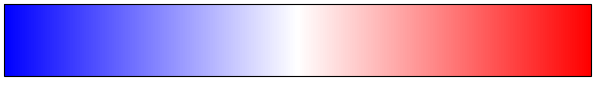
\includegraphics[width=\linewidth,height=0.15in,keepaspectratio]{../bin/colormaps/resource/matplotlib_bwr.png}}};
    %
    \node(apbslabel) [above, inner sep=6pt] at (spectrumbar.north) {30 kT/e};
    \node(apbslabel) [below, inner sep=6pt] at (spectrumbar.south) {-30 kT/e};       
    %
    %
    %
    \node(tetramer)[inner sep=0pt,right=2cm of spectrumbar.east]{\includegraphics[width=\linewidth,height=1.25in,keepaspectratio]{../results/cavity/output/tetramer_cavity_apbs_side_no_ramp_cropped.png}};
    %
    \node(captionB)[inner sep=0pt,above left] at (tetramer.north west) {\normalsize\textbf{\figurepanelb}};
    %
    \path (tetramer.north)++(-0.5,-0.95) coordinate (tetramerROISW1);            
    \path (tetramer.north)++(0.5,-1.8) coordinate (tetramerROINE1);
    \node(tetramerROIrect) [fit={(tetramerROISW1) (tetramerROINE1)}, dashedrectanglefit] {};
    %
    %
    \path (tetramer.west)++(-0.25,0.5) coordinate (chainA_tetramer);           
    \path (tetramer.north)++(-1.5,0) coordinate (chainB_tetramer);
    \path (tetramer.north)++(1.5,0) coordinate (chainAprime_tetramer);
    \path (tetramer.east)++(0.25,0.5) coordinate (chainBprime_tetramer);
    %
    \node(chainAlabel) [above, inner sep=2pt, align=center] at (chainA_tetramer) {Chain A};
    \node(chainBlabel) [above, inner sep=2pt, align=center] at (chainB_tetramer) {Chain B};
    \node(chainAprimelabel) [above, inner sep=2pt, align=center] at (chainAprime_tetramer) {Chain A'};
    \node(chainBprimelabel) [above, inner sep=2pt, align=center] at (chainBprime_tetramer) {Chain B'};
    %
    \node(D144_E174_closeup)[inner sep=0pt,below=1cm of tetramer.south,anchor=north]{\includegraphics[width=\linewidth,height=1.5in,keepaspectratio]{../results/cavity/output/tetramer_cavity_D144_E174_closeup_no_ramp_cropped.png}};
    %
    \node(closeuprectD144E174) [fit=(D144_E174_closeup), dashedrectanglefit] {};
    %
    \path[dashed edge] (tetramerROIrect.south) edge (closeuprectD144E174.north);
    %
    \path (D144_E174_closeup.south west)++(0.5,-0.65) coordinate (cE174label);
    \path (D144_E174_closeup.west)++(1.125,-0.65) coordinate (cE174);
    \node(E174) [above, inner sep=3pt, font=\small, font=\bfseries] at (cE174label) {E174};
    \path[-,thick] (E174.north) edge (cE174.south);
    %
    \path (D144_E174_closeup.south east)++(-0.5,-0.65) coordinate (cD144label);
    \path (D144_E174_closeup.east)++(-1.125,-0.3) coordinate (cD144);
    \node(D144) [above, inner sep=3pt, font=\small, font=\bfseries] at (cD144label) {D144};
    \path[-,thick] (D144.north) edge (cD144.south);
    %
    \node(filament)[inner sep=0pt,below=4.5cm of axialdimer.west,anchor=west]{\includegraphics[width=\linewidth,height=1.25in,keepaspectratio]{../results/cavity/output/filament_cavity_and_yb_blend_cutaway_cropped.png}};
    %
    \node(captionC)[inner sep=0pt,above left] at (filament.north west) {\normalsize\textbf{\figurepanelc}};
    %
\end{tikzcanvas}
\end{conditionalpanel}
\begin{conditionalcaption}
\caption[The electronegative lumen within the cardiac calsequestrin filament]{\textbf{\headingsubsectionsix}. \figurepanelcaptiona Left panel: the interior cavity of the dimer viewed down its long axis. Residues that interact with Yb atoms within the intra-dimer cleft (\maintextfigure~\ref{fig:intra_dimer_interface}) are shown as sticks. All other residues are rendered as surface. Right side: APBS-generated electrostatic surface of the same region. \figurepanelcaptionb The lumen is continuous down the length of filament because of the large solvent cavity formed at each dimer-dimer interface. The APBS-generated electrostatic surface of the lumen (as traced by HOLLOW using a 1.4 \AA\ probe) is shown, with closeup of residues D144 and E174 deep within the electronegative cavity. \figurepanelcaptionc View of the filament and its continuous interior cavity, with Yb sites shown as magenta spheres.}
\label{fig:filament_cavity}
\end{conditionalcaption}
\end{figure}
\begin{figure}[!h]
\centering
%\figuretitle{Figure~\ref{fig:inter_dimer_interface_cpvt}}
\begin{conditionalpanel}
    \begin{tikzcanvas}{}
        \node(overview1)[inner sep=0pt,below right]{\includegraphics[width=\linewidth,height=1.75in,keepaspectratio]{../results/inter_dimer_interface/output/tetramer_interface_overview_CPVT_cropped.png}};
        %
        \path (overview1.north)++(-1,-2.5) coordinate (S173SW1);            
        \path (overview1.north)++(-0.375,-1.75) coordinate (S173NE1);
        \node(S173one) [fit={(S173SW1) (S173NE1)}, dashedrectanglefit] {};
        %
        \path (overview1.north)++(0.375,-2.5) coordinate (S173SW2);           
        \path (overview1.north)++(1,-1.75) coordinate (S173NE2);
        \node(S173two) [fit={(S173SW2) (S173NE2)}, dashedrectanglefit] {};
        %
        %
        \path (overview1.north)++(-0.5,-1.75) coordinate (K180SW1);            
        \path (overview1.north)++(0,-1.125) coordinate (K180NE1);
        \node(K180one) [fit={(K180SW1) (K180NE1)}, dashedrectanglefit] {};
        %
        \path (overview1.north)++(0,-1.75) coordinate (K180SW2);           
        \path (overview1.north)++(0.5,-1.125) coordinate (K180NE2);
        \node(K180two) [fit={(K180SW2) (K180NE2)}, dashedrectanglefit] {};
        %
        \path (overview1.west)++(0,1) coordinate (chainA);           
        \path (overview1.north)++(-2.4,-0.5) coordinate (chainB);
        \path (overview1.north)++(2.4,-0.5) coordinate (chainAprime);
        \path (overview1.east)++(-0.25,1) coordinate (chainBprime);

        \node(chainAlabel) [above, inner sep=2pt, align=center] at (chainA) {Chain A};
        \node(chainBlabel) [above, inner sep=2pt, align=center] at (chainB) {Chain B};
        \node(chainAprimelabel) [above, inner sep=2pt, align=center] at (chainAprime) {Chain A'};
        \node(chainBprimelabel) [above, inner sep=2pt, align=center] at (chainBprime) {Chain B'};
        %
        %
        %
        \node(closeup180)[inner sep=0pt,below right,right=1.5cm of overview1]{\includegraphics[width=\linewidth,height=1.5in,keepaspectratio]{../results/inter_dimer_interface/output/tetramer_interface_K180_closeup_yb_cropped.png}};
        \node(closeup180rect) [fit=(closeup180), dashedrectanglefit] {};
        %
        \node(K180_ROI_label) [above, inner sep=5pt, align=center] at (closeup180.north) {D50/K180/E184/E187 Inter-Dimer Region};
        %
        \node(K180Rotator) at ([yshift=-1cm]K180_ROI_label.north) {\AxisRotator};
        \draw[line width=0.1ex] (K180Rotator.west) -- (K180Rotator.east);
        \node(K180RotatorLabel)[inner sep=4pt,right] at (K180Rotator.east) {\ang{60}};  
        %
        % E184 
        \path (closeup180.east)++(-1,-1.4)  coordinate (cE184);
        \node(E184_label) [above, inner sep=0pt, font=\small, font=\bfseries] at (cE184) {E184};
        % E187 
        \path (closeup180.east)++(-0.4,0.4) coordinate (cE187);
        \node(E187_label) [above, inner sep=0pt, font=\small, font=\bfseries] at (cE187) {E187};
        % D50
        \path (closeup180.west)++(0.75,0.4) coordinate (cD50);
        \node(D50_label) [above, inner sep=0pt, font=\small, font=\bfseries] at (cD50) {D50};
        % K180 
        \path (closeup180.west)++(2.2,0.3) coordinate (cK180);
        \node(K180) [above, inner sep=0pt, font=\small, font=\bfseries] at (cK180) {K180};
        %
        \path[dashed edge] (K180two.north east) edge (closeup180rect.north west);
        %
        %
        %
        \node(closeup173)[inner sep=0pt,below=3.5cm of overview1.south west,anchor=west]{\includegraphics[width=\linewidth,height=1.5in,keepaspectratio]{../results/inter_dimer_interface/output/tetramer_interface_S173_closeup_cropped.png}};
        \node(closeup173rect) [fit=(closeup173), dashedrectanglefit] {};
        %
        \node(S173_ROI_label) [above, inner sep=5pt, align=center] at (closeup173.north) {K87/S173/D325 Inter-Dimer Region};
        % S173
        \path (closeup173.west)++(1.5,0.25) coordinate (cS173);
        \node(S173) [above, inner sep=0pt, font=\small, font=\bfseries] at (cS173) {S173};
        % D325
        \path (closeup173.south)++(-1.25,+0.25) coordinate (cD325);
        \node(D325) [above, inner sep=0pt, font=\small, font=\bfseries] at (cD325) {D325}; 
        % D319
        \path (closeup173.south)++(2,1) coordinate (cD319);
        \node(D319) [above, inner sep=0pt, font=\small, font=\bfseries] at (cD319) {D319}; 
        % K87
        \path (closeup173.east)++(-1.25,0.5) coordinate (cK87);
        \node(K87) [above, inner sep=0pt, font=\small, font=\bfseries] at (cK87) {K87}; 
        % K172
        \path (closeup173.west)++(2.5,-0.4) coordinate (cK172);
        \node(K87) [above, inner sep=0pt, opacity=.4, font=\footnotesize, font=\bfseries] at (cK172) {K172}; 
        %
        \path[dashed edge] (S173one.south west) edge (closeup173rect.north west);
        %
        %
        %
        \node(D325A_plot)[inner sep=0pt,right=1.5cm of closeup173.east,anchor=west]{\input{../results/assembly_kinetics/output/kinetics_interface_mutation_D325A_D325I_85mM_K.pgf}};
        %
%        \node(closeuprectD325Aplot) [fit=(D325A_plot), dashedrectanglefit] {};
        %
%        \path[dashed edge] (closeup173rect.east) edge (closeuprectD325Aplot.west);
        %
        \node(captionA)[inner sep=10pt,above left] at (overview1.north west) {\normalsize\textbf{\figurepanela}};
        %
        \node(captionB)[inner sep=10pt,above left] at ([xshift=9cm]overview1.north west) {\normalsize\textbf{\figurepanelb}};
        %
        \node(captionC)[inner sep=10pt,above left] at (closeup173.north west) {\normalsize\textbf{\figurepanelc}};
        %
        \node(captionD)[inner sep=10pt,above left] at ([xshift=7cm]closeup173.north west) {\normalsize\textbf{\figurepaneld}};
    \end{tikzcanvas}
\end{conditionalpanel}
\begin{conditionalcaption}
\caption[The S173 and K180 residues are at the cardiac calsequestrin inter-dimer interface]{\textbf{\headingsubsectionseven}. \figurepanelcaptiona Inter-dimer interface residues in the vicinity of S173 and K180 shown as spheres. \figurepanelcaptionb Closeup of K180 with the adjacent E184 and E187 cation binding site, with the coordinated Yb atom shown as a sphere. \figurepanelcaptionc Hydrophilic pocket at S173. In this pocket, 3 different thioredoxin domains from 3 distinct chains interact (K87, S173, D325). K172 (backgrounded) is the most proximal of several residues that shield the pocket from bulk solvent. \figurepanelcaptiond Turbidity assay with the D325A and D325I mutations. All graphed values are mean of 3 technical replicates ± SD.}
\label{fig:inter_dimer_interface_cpvt}
\end{conditionalcaption}
\end{figure}
\begin{figure}[!h]
\centering
%\figuretitle{Figure~\ref{fig:graphical_summary}}
\begin{conditionalpanel}
    % All about specifying coords: https://stuff.mit.edu/afs/athena/contrib/tex-contrib/beamer/pgf-1.01/doc/generic/pgf/version-for-tex4ht/en/pgfmanualse8.html
    \tikzset{
        monomerA/.pic = {
            \draw[fill=orange,rounded corners] (-0.5,0)  
            -- ++(0.75,0) 
            -- ++(0.5,-1) 
            -- ++(-1.25,0) 
            -- cycle;
        }
    }
    \tikzset{
        monomerAmutantIntra/.pic = {
            \draw[fill=red,rounded corners] (-0.5,0) node(monomerAanchor)[inner sep=14] {}
            -- ++(0.75,0) 
            -- ++(0.5,-1) 
            -- ++(-1.25,0) 
            -- cycle;
            \draw[fill=LimeGreen,rounded corners] (-0.5,0) node(monomerAanchor2)[inner sep=14] {} 
            -- ++(0.625,0) 
            -- ++(0.5,-1) 
            -- ++(-1.125,0) 
            -- cycle;
            % Was previously using a start to indicate the mutant.
            % \node[star,star points=5, draw, fill=red,star point ratio=2.25,inner sep=0pt,minimum height=0.5cm] at ([xshift=-0.05cm]monomerAanchor.south east) {};
        }
    }
    \tikzset{
        monomerAmutantInter/.pic = {
            \draw[fill=red,rounded corners] (-0.5,0) node(monomerAanchor)[inner sep=14] {}
            -- ++(0.75,0) 
            -- ++(0.5,-1) 
            -- ++(-1.25,0) 
            -- cycle;
            \draw[fill=LimeGreen,rounded corners] (-0.375,0) node(monomerAanchor2)[inner sep=14] {} 
            -- ++(0.625,0) 
            -- ++(0.5,-1) 
            -- ++(-1.125,0) 
            -- cycle;
        }
    }
    % "B" chain
    \tikzset{
        monomerB/.pic = {
            \draw[fill=orange,rounded corners] (-0.5,0)  
            -- ++(1.25,0) 
            -- ++(0,-1) 
            -- ++(-0.75,0) 
            -- cycle;
        }
    }
    \tikzset{
        monomerBmutantIntra/.pic = {
            \draw[fill=red,rounded corners] (-0.5,0) node(monomerBanchor)[inner sep=14] {}
            -- ++(1.25,0) 
            -- ++(0,-1) 
            -- ++(-0.75,0) 
            -- cycle;
            \draw[fill=LimeGreen,rounded corners] (-0.375,0) node(monomerBanchor)[inner sep=14] {} 
            -- ++(1.125,0) 
            -- ++(0,-1) 
            -- ++(-0.625,0) 
            -- cycle;
        }
    }
    \tikzset{
        monomerBmutantInter/.pic = {
            \draw[fill=red,rounded corners] (-0.5,0) node(monomerBanchor)[inner sep=14] {}
            -- ++(1.25,0) 
            -- ++(0,-1) 
            -- ++(-0.75,0) 
            -- cycle;
            \draw[fill=LimeGreen,rounded corners] (-0.5,0) node(monomerBanchor)[inner sep=14] {} 
            -- ++(1.125,0) 
            -- ++(0,-1) 
            -- ++(-0.625,0) 
            -- cycle;
        }
    }
%     \begin{tikzcanvas}{}
%         % https://tex.stackexchange.com/questions/185279/anchoring-tikz-pics
%         %
%         \node(legendTitle)[align=center,font=\small,font=\bfseries, minimum size=2cm] at (current page.north) {Heterozygous Missense Genotypes};
%         \node(legendCenter)[align=center,below=0.125cm of legendTitle.south] {};
%         %
% %        \pic at ([xshift=-0.45cm,yshift=-0.6cm]legendWT.north) {monomerA};
% %        \pic at ([xshift=0.45cm,yshift=-0.6cm]legendWT.north) {monomerB};
%         %
%         \node(legendIntra)[left=1cm of legendCenter.west,align=center] {\textit{Intra}-Dimer Mutant};
%         %
%         \pic at ([xshift=-1cm,yshift=-0.6cm]legendIntra.north) {monomerA};
%         \node(X1)[align=center,color=red,font=\bfseries, font=\large, minimum size=2cm] at ([xshift=0cm,yshift=-0.7cm]legendIntra.south) {\Large \bf X};
%         \pic at ([xshift=0.75cm,yshift=-0.6cm]legendIntra.north) {monomerBmutantIntra};
%         %
%         \node(legendInter)[right=1cm of legendCenter.east,align=center] {\textit{Inter}-Dimer Mutant};
%         %
%         \pic at ([xshift=-0.45cm,yshift=-0.6cm]legendInter.north) {monomerA};
%         \pic at ([xshift=0.45cm,yshift=-0.6cm]legendInter.north) {monomerBmutantInter};
%         %
%         \draw[thick] ($(legendIntra.north west)+(-1,0.5)$) rectangle ($(legendInter.south east)+(1,-1.75)$);
%     \end{tikzcanvas}
%     \vspace{0.75cm}
    \begin{tikzcanvas}{}
        \node(genotypesLabel)[below right,align=center,font=\small,font=\bfseries] {Genotype};
        %
%        \node(chainTypesLabel)[right=2cm of genotypesLabel.east,align=center,font=\small,font=\bfseries, minimum size=2cm] {Protomers};
        %
        \node(retainedLabel)[right=0.9cm of genotypesLabel.east,align=center,font=\small,font=\bfseries] {Retained};
        % 
        \node(traffickedLabel)[right=1.7cm of retainedLabel.east,align=center,font=\small,font=\bfseries] {Exported};
        %
        % First separator
        %
        \path (genotypesLabel.south)++(-1,-0.25) coordinate (Separator1Left);
        \path (traffickedLabel.south)++(1.55,-0.25) coordinate (Separator1Right);
        \path[-] (Separator1Left) edge (Separator1Right);
        %
        %
        \node(hetIntraLabel)[below=1cm of genotypesLabel.south,align=center,font=\footnotesize] {Heterozygous\\\textit{Intra}-Dimer\\Mutant};
        %
        % \node(IntraChainTypes)[below=1cm of chainTypesLabel.south,align=center] {};
        % %
        % \pic at ([xshift=-0.75cm]IntraChainTypes.north) {monomerA};
        % \pic at ([xshift=0.75cm]IntraChainTypes.south) {monomerBmutantIntra};
        %
        \node(hetIntraHomoWT)[below=1cm of retainedLabel.south,align=center] {};
        %
        \pic at ([xshift=-0.45cm]hetIntraHomoWT.north) {monomerA};
        \pic at ([xshift=0.45cm]hetIntraHomoWT.north) {monomerB};
        \node(retainedPctIntra)[below=1cm of hetIntraHomoWT.south,align=center,font=\bfseries,font=\footnotesize] {\SI{50}{\percent}};
        %
        \node(hetIntraHomoMut)[align=center] at ([xshift=-0.2cm,yshift=-1.1cm]traffickedLabel.south) {};
        %
        \pic at ([xshift=-0.55cm]hetIntraHomoMut.north) {monomerAmutantIntra};
        \node(X2)[align=center,color=red,font=\large,font=\bfseries, minimum size=2cm] at ([xshift=0.3cm,yshift=-0.3cm]hetIntraHomoMut.south) {\normalsize \bf X};
        \pic at ([xshift=0.85cm]hetIntraHomoMut.north) {monomerBmutantIntra};
        %
        %
        %
        \path (genotypesLabel.south)++(-1,-3) coordinate (separator2Left);
        \path (traffickedLabel.south)++(1.55,-3) coordinate (separator2Right);
        \path[-] (separator2Left) edge (separator2Right);
        %
        %
        %
        \node(hetInterLabel)[below=3.5cm of genotypesLabel.south,align=center,font=\footnotesize] {Heterozygous\\\textit{Inter}-Dimer\\Mutant};
        %
        % \node(hetInterChainTypes)[below=3.5cm of chainTypesLabel.south,align=center] {};
        % %
        % \pic at ([xshift=-0.75cm]hetInterChainTypes.north) {monomerA};
        % \pic at ([xshift=0.75cm]hetInterChainTypes.south) {monomerBmutantInter};
        %
        % Retained
        %
        \node(hetInterHomoWT)[below=3.5cm of retainedLabel.south,align=center] {};
        %
        \pic at ([xshift=-0.45cm]hetInterHomoWT.north) {monomerA};
        \pic at ([xshift=0.45cm]hetInterHomoWT.north) {monomerB};
        \node(retainedPctInter)[below=1cm of hetInterHomoWT.south,align=center,font=\bfseries,font=\footnotesize] {\SI{25}{\percent}};
        %
        % Exported
        %
        \node(hetInterHet1)[below=3.5cm of traffickedLabel.south,align=center] {};
        %
        \pic at ([xshift=-0.45cm]hetInterHet1.north) {monomerA};
        \pic at ([xshift=0.45cm]hetInterHet1.north) {monomerBmutantInter};

        \node(hetInterHet2)[below=1.25cm of hetInterHet1.south,align=center] {};

        \pic at ([xshift=-0.45cm]hetInterHet2.north) {monomerAmutantInter};
        \pic at ([xshift=0.45cm]hetInterHet2.north) {monomerB};

        \node(hetInterHomoMut)[below=1.25cm of hetInterHet2.south,align=center] {};

        \pic at ([xshift=-0.45cm]hetInterHomoMut.north) {monomerAmutantInter};
        \pic at ([xshift=0.45cm]hetInterHomoMut.north) {monomerBmutantInter};
        %
        %
        %
        %
        % https://tex.stackexchange.com/questions/185279/anchoring-tikz-pics
        %
        \node(legendTitle)[align=center,font=\small,font=\bfseries, minimum size=2cm] at ([xshift=0.6cm,yshift=3.5cm]retainedLabel.north) {Heterozygous Missense Genotypes};
        \node(legendCenter)[align=center,below=0.125cm of legendTitle.south] {};
        %
%        \pic at ([xshift=-0.45cm,yshift=-0.6cm]legendWT.north) {monomerA};
%        \pic at ([xshift=0.45cm,yshift=-0.6cm]legendWT.north) {monomerB};
        %
        \node(legendIntra)[left=1cm of legendCenter.west,align=center] {\textit{Intra}-Dimer Mutant};
        %
        \pic at ([xshift=-0.55cm,yshift=-0.6cm]legendIntra.north) {monomerA};
        \node(X1)[align=center,color=red,font=\bfseries, font=\large, minimum size=2cm] at ([xshift=0.3cm,yshift=-0.7cm]legendIntra.south) {\normalsize \bf X};
        \pic at ([xshift=0.85cm,yshift=-0.6cm]legendIntra.north) {monomerBmutantIntra};
        %
        \node(legendInter)[right=1cm of legendCenter.east,align=center] {\textit{Inter}-Dimer Mutant};
        %
        \pic at ([xshift=-0.45cm,yshift=-0.6cm]legendInter.north) {monomerA};
        \pic at ([xshift=0.45cm,yshift=-0.6cm]legendInter.north) {monomerBmutantInter};
        %
        \draw[thick] ($(legendIntra.north west)+(-1,0.5)$) rectangle ($(legendInter.south east)+(1,-1.75)$);
    \end{tikzcanvas}
\end{conditionalpanel}
\begin{conditionalcaption}
\caption[Disease inheritance patterns differ by location of mutation]{\textbf{Heterozygously-carried mutations at different calsequestrin interfaces have different disease inheritance patterns.} Mutations that inhibit dimerization are likely to cause penetrant disease only when carried recessively - a consequence of export of mutant monomers from the SR. However, mutations that inhibit \textit{inter}-dimer interaction are likely to have dominant effect - a consequence of the fact that only \SI{25}{\percent} of dimers remain functional for the purpose of filamentation.}
\label{fig:graphical_summary}
\end{conditionalcaption}
\end{figure}

\clearpage % help to get the table onto a new page
\section{} % Tables
\setcounter{table}{0}
\renewcommand{\thetable}{\arabic{table}}
\begin{table}[hp]
\footnotesize
\caption[Crystallographic Data Collection and Refinement]{\textbf{Crystallographic Data Collection and Refinement}}
\label{tab:table_xtal_stats}
\begin{table}[hp]
\footnotesize
\caption[Crystallographic Data Collection and Refinement]{\textbf{Crystallographic Data Collection and Refinement}}
\label{tab:table_xtal_stats}
\input{../results/table_one/output/table_xtal_stats.tex}
\end{table}

\end{table}

\clearpage % help to get the extended data onto a new page
\section{} % Extended Data Figures
\setcounter{figure}{0}
\setcounter{table}{0}
\renewcommand{\figurename}{Extended Data Fig.}
\renewcommand{\tablename}{Extended Data Table}
\renewcommand{\thefigure}{\arabic{figure}}
\renewcommand{\thetable}{\arabic{table}}
\begin{figure}[!h]
\centering
%\figuretitle{Figure~\ref{fig:biochemistry_supplement}}
\begin{conditionalpanel}
    \begin{tikzcanvas}{}
        \node(WT_EDTA_plot)[inner sep=0pt,above right]{\input{../results/assembly_kinetics/output/kinetics_WT_EDTA.pgf}};
        %
        \node(captionA)[inner sep=0pt,above left] at (WT_EDTA_plot.north west) {\normalsize\textbf{\figurepanela}};
        %
        \node(S173I_No_K_plot)[inner sep=0pt,right=1.25cm of WT_EDTA_plot.east, anchor=west]{\input{../results/assembly_kinetics/output/kinetics_CPVT_mutation_S173I_0mM_K.pgf}};
        %
        \node(captionB)[inner sep=0pt,above left] at (S173I_No_K_plot.north west) {\normalsize\textbf{\figurepanelb}};
        %
    \end{tikzcanvas}
\end{conditionalpanel}
\begin{conditionalcaption}
\caption[Multimerization kinetics of the S173I mutant observed in 0 mM KCl]{\textbf{Turbidity assay controls; related to \maintextfigure~\ref{fig:S173I_genetics_and_biochemistry}.} \figurepanelcaptiona Stoichiometric addition of EDTA demonstrates immediate reversal of calcium-induced turbidity. \figurepanelcaptionb Turbidity assay for the S173I mutant in \SI{0}{\milli\Molar} KCl. All graphed values are mean of 3 technical replicates ± SD.}
\label{fig:biochemistry_extended}
\end{conditionalcaption}
\end{figure}
\begin{figure}[!h]
\centering
\newcommand{\tetramerheight}{1.125in}
%\figuretitle{Figure~\ref{fig:inter_dimer_interface_BSA_comparison}}
\begin{conditionalpanel}
    \begin{tikzcanvas}{}
        \node(deo_native)[inner sep=0pt, below right] {\includegraphics[width=\linewidth,height=\tetramerheight,keepaspectratio]{../results/inter_dimer_comparison/output/tetramer_deo_native_oriented_cropped.png}};
        %
        \node (deo_native_table) [inner sep=10pt,anchor=north] at (deo_native.south) {
            \begin{tabular}{c c}
                Interface Chains & BSA (\AA\textsuperscript{2}) \\
                \hline
                \input{../results/inter_dimer_comparison/output/table_interface_comparison_tetramer_deo_native.tex}
                % B, A’ & 734.0 \\
                % A, A’ & 382.0 \\
                % B, B’ & 381.0 \\
                % A, B’ & 101.0
            \end{tabular}
        };
        %
        \node(6OVW_label) [above, inner sep=3pt, align=center] at (deo_native.north) {6OVW (This Study)\\Similar: 6OWW};
        %
        \node(1a8y)[inner sep=0pt,right=0.8cm of deo_native] {\includegraphics[width=\linewidth,height=\tetramerheight,keepaspectratio]{../results/inter_dimer_comparison/output/tetramer_1a8y_oriented_cropped.png}};
        %
        \node(1a8y_label) [above, inner sep=3pt, align=center] at (1a8y.north) {1A8Y\\Similar: 3TRP, 3TRQ, 3US3, 3V1W, 5CRD, 5KN0, 5KN3};
        %
        \node (1a8y_table) [inner sep=10pt,anchor=north] at (1a8y.south) {
            \begin{tabular}{c c}
                Interface Chains & BSA (\AA\textsuperscript{2}) \\
                \hline
                \input{../results/inter_dimer_comparison/output/table_interface_comparison_tetramer_1a8y.tex}
            \end{tabular}
        };
        %
        \node(1sji)[inner sep=0pt,right=0.8cm of 1a8y] {\includegraphics[width=\linewidth,height=\tetramerheight,keepaspectratio]{../results/inter_dimer_comparison/output/tetramer_1sji_oriented_cropped.png}};
        %
        \node(1sji_label) [above, inner sep=3pt, align=center] at (1sji.north) {1SJI};
        %
        \node (1sji_table) [inner sep=10pt,anchor=north] at (1sji.south) {
            \begin{tabular}{c c}
                Interface Chains & BSA (\AA\textsuperscript{2}) \\
                \hline
                \input{../results/inter_dimer_comparison/output/table_interface_comparison_tetramer_1sji.tex}
            \end{tabular}
        };
        %
        %
        %
        \node(2vaf)[inner sep=0pt,below=7cm of deo_native.west,anchor=west] {\includegraphics[width=\linewidth,height=\tetramerheight,keepaspectratio]{../results/inter_dimer_comparison/output/tetramer_2vaf_oriented_cropped.png}};
        %
        \node(2vaf_label) [above, inner sep=3pt, align=center] at (2vaf.north) {2VAF};
        %
        \node (2vaf_table) [inner sep=10pt,anchor=north] at (2vaf.south) {
            \begin{tabular}{c c}
                Interface Chains & BSA (\AA\textsuperscript{2}) \\
                \hline
                \input{../results/inter_dimer_comparison/output/table_interface_comparison_tetramer_2vaf.tex}
            \end{tabular}
        };
        %
        \node(3uom)[inner sep=0pt,below=7cm of 1a8y.west,anchor=west] {\includegraphics[width=\linewidth,height=\tetramerheight,keepaspectratio]{../results/inter_dimer_comparison/output/tetramer_3uom_oriented_cropped.png}};
        %
        \node(3uom_label) [above, inner sep=3pt, align=center] at (3uom.north) {3UOM};
        %
        \node (3uom_table) [inner sep=10pt,anchor=north] at (3uom.south) {
            \begin{tabular}{c c}
                Interface Chains & BSA (\AA\textsuperscript{2}) \\
                \hline
                \input{../results/inter_dimer_comparison/output/table_interface_comparison_tetramer_3uom.tex}
            \end{tabular}
        };
        %
        \node(5cre)[inner sep=0pt,below=7cm of 1sji.west,anchor=west] {\includegraphics[width=\linewidth,height=\tetramerheight,keepaspectratio]{../results/inter_dimer_comparison/output/tetramer_5cre_oriented_cropped.png}};
        %
        \node(5cre_label) [above, inner sep=3pt, align=center] at (5cre.north) {5CRE};
        %
        \node (5cre_table) [inner sep=10pt,anchor=north] at (5cre.south) {
            \begin{tabular}{c c}
                Interface Chains & BSA (\AA\textsuperscript{2}) \\
                \hline
                \input{../results/inter_dimer_comparison/output/table_interface_comparison_tetramer_5cre.tex}
            \end{tabular}
        };
        %
        %
        %
        \node(5crg)[inner sep=0pt,below=7cm of 2vaf.west,anchor=west] {\includegraphics[width=\linewidth,height=\tetramerheight,keepaspectratio]{../results/inter_dimer_comparison/output/tetramer_5crg_oriented_cropped.png}};
        %
        \node(5crg_label) [above, inner sep=3pt, align=center] at (5crg.north) {5CRG\\Similar: 5CRH};
        %
        \node (5crg_table) [inner sep=10pt,anchor=north] at (5crg.south) {
            \begin{tabular}{c c}
                Interface Chains & BSA (\AA\textsuperscript{2}) \\
                \hline
                \input{../results/inter_dimer_comparison/output/table_interface_comparison_tetramer_5crg.tex}
            \end{tabular}
        };
        %
        \node(5kn1)[inner sep=0pt,below=7cm of 3uom.west,anchor=west] {\includegraphics[width=\linewidth,height=\tetramerheight,keepaspectratio]{../results/inter_dimer_comparison/output/tetramer_5kn1_oriented_cropped.png}};
        %
        \node(5kn1_label) [above, inner sep=3pt, align=center] at (5kn1.north) {5KN1\\Similar: 5KN2};
        %
        \node (5kn1_table) [inner sep=10pt,anchor=north] at (5kn1.south) {
            \begin{tabular}{c c}
                Interface Chains & BSA (\AA\textsuperscript{2}) \\
                \hline
                \input{../results/inter_dimer_comparison/output/table_interface_comparison_tetramer_5kn1.tex}
            \end{tabular}
        };
        %
    \end{tikzcanvas}
\end{conditionalpanel}
\begin{conditionalcaption}
\caption[Comparison of buried surface area (BSA) at putative dimer-dimer multimerization interfaces observed in all published calsequestrin structures]{\textbf{The \textit{inter}-dimer interface of the new candidate cardiac calsequestrin filament exhibits all-by-all contacts and greater buried surface area (BSA) compared to all other published calsequestrin structures; related to \maintextfigure~\ref{fig:filament_overview}.} For each published calsequestrin structure, the inter-dimer interface with the greatest buried surface area is shown. Residues with buried surface area at the interface are rendered as spheres. Where similar PDB codes are listed, inter-dimer interfaces are roughly isomorphous with the example structure shown, although the space group and unit cell used to determine the structure sometimes differ.} 
\label{fig:inter_dimer_interface_BSA_comparison}
\end{conditionalcaption}
\end{figure}
\begin{figure}[!h]
\centering
%\figuretitle{Figure~\ref{fig:filament_comparison}}
\begin{conditionalpanel}
    \begin{tikzcanvas}{}
        \node(filament_native)[inner sep=0pt,below right]{\includegraphics[width=2.8in,keepaspectratio]{../results/filament_comparison/output/filament_deo_native_spheres_cropped.png}};
        %
        \node(filament_caption)[above, inner sep=7pt] at (filament_native.north) {6OWV, Human Cardiac Calsequestrin (This Study)};
        %
        \node(globes_6OWV)[inner sep=0pt,right=1cm of filament_native]{\includegraphics[width=2.8in,keepaspectratio]{../results/filament_comparison/output/filament_deo_native_thioredoxin_globes_cropped.png}};
        %
        \node(captionA)[inner sep=0pt,above left] at (filament_native.north west) {\normalsize\textbf{\figurepanela}};
        %
        %
        %
        \node(filament_1a8y)[inner sep=0pt,below=4cm of filament_native.west,anchor=west]{\includegraphics[width=2.8in,keepaspectratio]{../results/filament_comparison/output/filament_1a8y_spheres_cropped.png}};
        %
        \node(filament_caption)[above, inner sep=7pt] at (filament_1a8y.north) {1A8Y, Rabbit Skeletal Calsequestrin (1998)};
        %
        \node(globes_1a8y)[inner sep=0pt,right=1cm of filament_1a8y]{\includegraphics[width=2.8in,keepaspectratio]{../results/filament_comparison/output/filament_1a8y_thioredoxin_globes_cropped.png}};
        %
        \node(captionB)[inner sep=0pt,above left] at (filament_1a8y.north west) {\normalsize\textbf{\figurepanelb}};
        %
        %
        %
        \node(filament_1sji)[inner sep=0pt,below=4.5cm of filament_1a8y.west,anchor=west]{\includegraphics[width=2.8in,keepaspectratio]{../results/filament_comparison/output/filament_1sji_spheres_cropped.png}};
        %
        \node(filament_caption)[above, inner sep=7pt] at (filament_1sji.north) {1SJI, Canine Cardiac Calsequestrin (2005)};
        %
        \node(globes_1sji)[inner sep=0pt,right=1cm of filament_1sji]{\includegraphics[width=2.8in,keepaspectratio]{../results/filament_comparison/output/filament_1sji_thioredoxin_globes_cropped.png}};
        %
        \node(captionC)[inner sep=0pt,above left] at (filament_1sji.north west) {\normalsize\textbf{\figurepanelc}};
    \end{tikzcanvas}
\end{conditionalpanel}
\begin{conditionalcaption}
\caption[Comparison of the new filament candidate to prior structures]{\textbf{\headingsubsectionthree}. \figurepanelcaptiona The new candidate cardiac calsequestrin filament assembled from crystallographic symmetry operations on PDB ID 6OWV (human CASQ2, this study). The new candidate CASQ2 filament exhibits tight packing of protomers and thioredoxin domains (shown on the right using equal-size spheres placed at the center of mass of each thioredoxin domain). \figurepanelcaptionb A putative skeletal calsequestrin filament assembled from crystallographic symmetry operations on PDB ID 1A8Y (rabbit CASQ1, 1998). Right-side: equal-size spheres represent thioredoxin domains. \figurepanelcaptionc A putative skeletal calsequestrin filament assembled from crystallographic symmetry operations on PDB ID 1SJI (canine CASQ2, 2005). Right-side: equal-size spheres represent thioredoxin domains.}
\label{fig:filament_comparison}
\end{conditionalcaption}
\end{figure}
\begin{figure}[!h]
\centering
%\figuretitle{Figure~\ref{fig:intra_dimer_interface_maps}}
\begin{conditionalpanel}
    \begin{tikzcanvas}{}
        %
        \node(E143nativemap)[inner sep=0pt,below right]{\includegraphics[width=1.75in,keepaspectratio]{../results/dimer_interface/output/dimer_interface_E143_closeup_native_map_cropped.png}};
        %
        \node(D140_E143_E147_ROI_label) [above, inner sep=5pt, align=center] at (E143nativemap.north) {D140/E143/E147 Intra-Dimer Region};
        %
        % D140
        \path (E143nativemap.north)++(1.3,-0.4)  coordinate (cD140);
        \node(D140) [above, inner sep=0pt, font=\small, font=\bfseries] at (cD140) {D140};
        % E143
        \path (E143nativemap.north)++(-1.9,-1)  coordinate (cE143);
        \node(E143) [above, inner sep=0pt, font=\small, font=\bfseries] at (cE143) {E143};
        % E275
        \path (E143nativemap.east)++(-0.75,0)  coordinate (cE275);
        \node(E275) [above, inner sep=0pt, font=\small, font=\bfseries] at (cE275) {E275};
        % E147
        \path (E143nativemap.west)++(0.5,-0.75)  coordinate (cE147);
        \node(E147) [above, inner sep=0pt, font=\small, font=\bfseries] at (cE147) {E147};
        % D278
        \path (E143nativemap.east)++(-0.9,-0.75)  coordinate (cD278);
        \node(D278) [above, inner sep=0pt, font=\small, font=\bfseries] at (cD278) {D278};
        % D280
        \path (E143nativemap.south)++(1,0.35)  coordinate (cD280);
        \node(D280) [above, inner sep=0pt, font=\small, font=\bfseries] at (cD280) {D280};
        %
        %
        \node(belowcaption)[below, inner sep=5pt] at (E143nativemap.south) {Native map at 1.5 $\sigma$};
        %
        \node(E143ybmap)[inner sep=0pt,right=1cm of E143nativemap]{\includegraphics[width=1.75in,keepaspectratio]{../results/dimer_interface/output/dimer_interface_E143_closeup_yb_map_cropped.png}};
        %
        \node(belowcaption)[below, inner sep=5pt] at (E143ybmap.south) {Yb-complexed map at 1.5 $\sigma$};
        %
        \node(E143anommap)[inner sep=0pt,right=0cm and 1cm of E143ybmap]{\includegraphics[width=1.75in,keepaspectratio]{../results/dimer_interface/output/dimer_interface_E143_closeup_yb_map_anom_cropped.png}};
        %
        \node(belowcaption)[below, inner sep=5pt] at (E143anommap.south) {Yb-complexed anomalous map at 3.0 $\sigma$};
        %
        %
        %
        %
        \node(D310nativemap)[inner sep=0pt,below=1.5cm of E143nativemap.south west,anchor=north west]{\includegraphics[width=1.75in,keepaspectratio]{../results/dimer_interface/output/dimer_interface_D310_closeup_native_map_cropped.png}};
        %
        \node(D310_ROI_label) [above, inner sep=5pt, align=center] at (D310nativemap.north) {D310 Intra-Dimer Region};
        % D310
        \path (D310nativemap.north)++(0,-0.5)  coordinate (cD310);
        \node(D310) [above, inner sep=0pt, font=\small, font=\bfseries] at (cD310) {D310};
        % R251_L
        \path (D310nativemap.west)++(0.5,-0.8)  coordinate (cR251_L);
        \node(R251_L) [above, inner sep=0pt, font=\small, font=\bfseries] at (cR251_L) {R251};
        % R251_R
        \path (D310nativemap.east)++(-0.5,-0.8)  coordinate (cR251_R);
        \node(R251_R) [above, inner sep=0pt, font=\small, font=\bfseries] at (cR251_R) {R251};
        % K276
        \path (D310nativemap.south)++(0,0.25)  coordinate (cK276);
        \node(K276) [above, inner sep=0pt, font=\small, font=\bfseries] at (cK276) {K276};
        %
        %
        \node(belowcaption)[below, inner sep=5pt] at (D310nativemap.south) {Native map at 1.5 $\sigma$};
        %
        \node(D310ybmap)[inner sep=0pt,right=1cm of D310nativemap]{\includegraphics[width=1.75in,keepaspectratio]{../results/dimer_interface/output/dimer_interface_D310_closeup_yb_map_cropped.png}};
        %
        \node(belowcaption)[below, inner sep=5pt] at (D310ybmap.south) {Yb-complexed map at 1.5 $\sigma$};
        %
        \node(D310anommap)[inner sep=0pt,right=1cm of D310ybmap]{\includegraphics[width=1.75in,keepaspectratio]{../results/dimer_interface/output/dimer_interface_D310_closeup_yb_map_anom_cropped.png}};
        %
        \node(belowcaption)[below, inner sep=5pt] at (D310anommap.south) {Yb-complexed anomalous map at 3.0 $\sigma$};
        %
        %
        %
        %
        \node(captionA)[inner sep=5pt,above left] at (E143nativemap.north west) {\normalsize\textbf{\figurepanela}};
        \node(captionB)[inner sep=5pt,above left] at (D310nativemap.north west) {\normalsize\textbf{\figurepanelb}};
    \end{tikzcanvas}
\end{conditionalpanel}
\begin{conditionalcaption}
\caption[Maps for Yb-Binding Sites at the Cardiac Calsequestrin Intra-Dimer Interface]{\textbf{Electron density and anomalous difference maps for Yb-binding sites at the cardiac calsequestrin \textit{intra}-dimer interface; related to \maintextfigure~\ref{fig:intra_dimer_interface}.} \figurepanelcaptiona Electron density and anomalous difference maps for the D140-E143-E147 region of interest. \figurepanelcaptionb Electron density and anomalous difference maps for the D310 region of interest.}
\label{fig:intra_dimer_interface_maps}
\end{conditionalcaption}
\end{figure}





\begin{figure}[!h]
\centering
%\figuretitle{Figure~\ref{fig:intra_dimer_interface_6OVW_vs_other_overlay}}
\begin{conditionalpanel}
    \begin{tikzcanvas}{}
        %
        % 2VAF
        \node(pdb_2vaf)[inner sep=0pt,below right]{\includegraphics[height=0.75in,keepaspectratio]{../results/dimer_interface/output/dimer_interface_overlay_2vaf_cropped.png}};
        %
        \node(pdb_2vaf_caption)[below, inner sep=5pt,align=center] at (pdb_2vaf.south) {2VAF\\None (\SI{2}{\Molar} \ch{NaCl})};
        %
        % 3UOM
        \node(pdb_3uom)[inner sep=0pt,right=1cm of pdb_2vaf]{\includegraphics[height=0.75in,keepaspectratio]{../results/dimer_interface/output/dimer_interface_overlay_3uom_cropped.png}};
        %
        \node(pdb_3uom_caption)[below, inner sep=5pt,align=center] at (pdb_3uom.south) {3UOM\\\SI{50}{\milli\Molar} \ch{CaCl2}};
        %
        % 5CRG
        \node(pdb_5crg)[inner sep=0pt,right=1cm of pdb_3uom]{\includegraphics[height=0.75in,keepaspectratio]{../results/dimer_interface/output/dimer_interface_overlay_5crg_cropped.png}};
        %
        \node(pdb_5crg_caption)[below, inner sep=5pt,align=center] at (pdb_5crg.south) {5CRG\\\SI{10}{\milli\Molar} \ch{CaCl2}};
        %
        %
        %
        % 5CRH
        \node(pdb_5crh)[inner sep=0pt,below=1cm of pdb_2vaf]{\includegraphics[height=0.75in,keepaspectratio]{../results/dimer_interface/output/dimer_interface_overlay_5crh_cropped.png}};
        %
        \node(pdb_5crh_caption)[below, inner sep=5pt,align=center] at (pdb_5crh.south) {5CRH\\\SI{5}{\milli\Molar} \ch{CaCl2}};
        %
        % 5KN1
        \node(pdb_5kn1)[inner sep=0pt,right=1cm of pdb_5crh]{\includegraphics[height=0.75in,keepaspectratio]{../results/dimer_interface/output/dimer_interface_overlay_5kn1_cropped.png}};
        %
        \node(pdb_5kn1_caption)[below, inner sep=5pt,align=center] at (pdb_5kn1.south) {5KN1\\\SI{5}{\milli\Molar} \ch{CaCl2}};
        %
        % 5KN2
        \node(pdb_5kn2)[inner sep=0pt,right=1cm of pdb_5kn1]{\includegraphics[height=0.75in,keepaspectratio]{../results/dimer_interface/output/dimer_interface_overlay_5kn2_cropped.png}};
        %
        \node(pdb_5kn2_caption)[below, inner sep=5pt,align=center] at (pdb_5kn2.south) {5KN2\\\SI{5}{\milli\Molar} \ch{CaCl2}};
        %
        %
        % Journal says rotated text not allowed: Tightly-packed dimers from published calsequestrin structures overlaid onto the tightly-packed cardiac calsequestrin dimer from this study (6OVW)
        \draw [decorate,decoration={brace,amplitude=10pt,mirror,raise=4pt},yshift=0pt] ([shift={(0.5cm,0cm)}]pdb_5kn2.south east) -- ([shift={(0.5cm,2.75cm)}]pdb_5kn2.north east) node [black,midway,xshift=1.75cm,text width=3.5cm,rotate=-90] {};
        %
        \draw[] ([yshift=-1.25cm]pdb_5crh.south west) -- ([yshift=-1.25cm]pdb_5kn2.south east);
        %
        %
        %
        % 1A8Y
        \node(pdb_1a8y)[inner sep=0pt,below=2cm of pdb_5crh]{\includegraphics[height=0.75in,keepaspectratio]{../results/dimer_interface/output/dimer_interface_overlay_1a8y_cropped.png}};
        %
        \node(pdb_1a8y_caption)[below, inner sep=5pt,align=center] at (pdb_1a8y.south) {1A8Y\\None};
        %
        % 1SJI
        \node(pdb_1sji)[inner sep=0pt,right=1cm of pdb_1a8y]{\includegraphics[height=0.75in,keepaspectratio]{../results/dimer_interface/output/dimer_interface_overlay_1sji_cropped.png}};
        %
        \node(pdb_1sji_caption)[below, inner sep=5pt,align=center] at (pdb_1sji.south) {1SJI\\None};
        %
        % 3TRP
        \node(pdb_3trp)[inner sep=0pt,right=1cm of pdb_1sji]{\includegraphics[height=0.75in,keepaspectratio]{../results/dimer_interface/output/dimer_interface_overlay_3trp_cropped.png}};
        %
        \node(pdb_3trp_caption)[below, inner sep=5pt,align=center] at (pdb_3trp.south) {3TRP\\\SI{2}{\milli\Molar} \ch{CaCl2} or \ch{SrCl2}};
        %
        % 3TRQ
        \node(pdb_3trq)[inner sep=0pt,right=1cm of pdb_3trp]{\includegraphics[height=0.75in,keepaspectratio]{../results/dimer_interface/output/dimer_interface_overlay_3trq_cropped.png}};
        %
        \node(pdb_3trq_caption)[below, inner sep=5pt,align=center] at (pdb_3trq.south) {3TRQ\\None};
        %
        %
        %
        % 3US3
        \node(pdb_3us3)[inner sep=0pt,below=1cm of pdb_1a8y]{\includegraphics[height=0.75in,keepaspectratio]{../results/dimer_interface/output/dimer_interface_overlay_3us3_cropped.png}};
        %
        \node(pdb_3us3_caption)[below, inner sep=5pt,align=center] at (pdb_3us3.south) {3US3\\None};
        %
        % 3V1W
        \node(pdb_3v1w)[inner sep=0pt,right=1cm of pdb_3us3]{\includegraphics[height=0.75in,keepaspectratio]{../results/dimer_interface/output/dimer_interface_overlay_3v1w_cropped.png}};
        %
        \node(pdb_3v1w_caption)[below, inner sep=5pt,align=center] at (pdb_3v1w.south) {3V1W\\Unpublished};
        %
        % 5CRD
        \node(pdb_5crd)[inner sep=0pt,right=1cm of pdb_3v1w]{\includegraphics[height=0.75in,keepaspectratio]{../results/dimer_interface/output/dimer_interface_overlay_5crd_cropped.png}};
        %
        \node(pdb_5crd_caption)[below, inner sep=5pt,align=center] at (pdb_5crd.south) {5CRD\\None};
        %
        % 5CRE
        \node(pdb_5cre)[inner sep=0pt,right=1cm of pdb_5crd]{\includegraphics[height=0.75in,keepaspectratio]{../results/dimer_interface/output/dimer_interface_overlay_5cre_cropped.png}};
        %
        \node(pdb_5cre_caption)[below, inner sep=5pt,align=center] at (pdb_5cre.south) {5CRE\\None};
        %
        %
        %
        % 5KN0
        \node(pdb_5kn0)[inner sep=0pt,below=1cm of pdb_3us3]{\includegraphics[height=0.75in,keepaspectratio]{../results/dimer_interface/output/dimer_interface_overlay_5kn0_cropped.png}};
        %
        \node(pdb_5kn0_caption)[below, inner sep=5pt,align=center] at (pdb_5kn0.south) {5KN0\\None};
        %
        % 5KN3
        \node(pdb_5kn3)[inner sep=0pt,right=1cm of pdb_5kn0]{\includegraphics[height=0.75in,keepaspectratio]{../results/dimer_interface/output/dimer_interface_overlay_5kn3_cropped.png}};
        %
        \node(pdb_5kn3_caption)[below, inner sep=5pt,align=center] at (pdb_5kn3.south) {5KN3\\None};
        %
        %
        % Journal says rotated text not allowed. Loosely-packed dimers from published calsequestrin structures overlaid onto the tightly-packed cardiac calsequestrin dimer from this study (6OVW)
        \draw [decorate,decoration={brace,amplitude=10pt,mirror,raise=4pt},yshift=0pt] ([shift={(0.5cm,-6cm)}]pdb_3trq.south east) -- ([shift={(0.5cm,0cm)}]pdb_3trq.north east) node [black,midway,xshift=1.75cm,text width=3.5cm,rotate=-90] {};
        %
    \end{tikzcanvas}
\end{conditionalpanel}
\begin{conditionalcaption}
\caption[Overlays of dimers from published calsequestrin structures]{\textbf{Dimer overlays reveal that all published calsequestrin structures can be classified into tightly packed or loosely packed dimers; related to \maintextfigure~\ref{fig:intra_dimer_interface}.} Dimers from published calsequestrin structures (lighter orange and green) are overlaid onto the tightly packed dimer from this study (6OVW, darker orange and green). In each dimer pair, chain A is aligned to chain A to illustrate the relative displacement of chain B. The concentration of divalent cations used in the crystallization condition is noted below. The overlays reveal two distinct conformational groupings. The more tightly packed conformation with inwardly rotated chains resembles the dimer in this study and appears to form at low pH or in the presence of neutralizing divalents.}
\label{fig:intra_dimer_interface_6OVW_vs_other_overlay}
\end{conditionalcaption}
\end{figure}

% Group 1 - Compact group. native: low pH, 2VAF: 2 M NaCl, all others: > 5 mM Ca before mixing, and Ca was pre-soaked in or dialyzed in.
% Group 2 - Characterized by low or no divalent cations. 3trp is the only structure with divalent cations, and only at 2 mM (less after mixing with well solution).
%
% In more detail, most of the conditions describe either mother liquor or the protein, so need to infer the the final concentration after mixing:
% 2vaf: 2 M NaCl and 10% (w/v) PEG 6000
% 1sji: 15% polyethylene glycol 400, 50 mM sodium citrate, 0.25% n-dodecyl- -D-maltoside, and 0.1 M Tris-HCl at pH 8.5.
% 1a8y: 10% MPD, 0.1 M Na3 citrate, 0.050 M Na cacodylate, pH 6.5
% 3trp, 50 m M HEPES (pH 7.0), 0.1 M NaCl, 2 mM CaCl2 or SrCl2, and 14% 2-methyl-2,4-pentanediol.
% 3uom, 50 mM BisTris propane (pH 5.5), 50 mM CaCl2, and 23% 2-methyl-2,4-pentanediol.
% 3us3, MPD but conditions not given. No indication of using Ca
% 3trq, MPD but conditions not given. No indication of using Ca
% 5crd: 0.1 M HEPES, 0.2 M NaCl, 27.5% (v/v) 2-methyl-2,4-pentanediol, pH 7.0
% 5cre: hCasq1 same as above
% 5crg: hCasq1 10 mM CaCl2 diffused into same buffer.
% 5crh: M87T, protein started in 5 mM CaCl2, final concentration < half that after mixing drop. Same mother liquor as above.
% 5kn0, "Low-Ca2+" (actually no Ca++) Native Bovine Casq1, mixed 1:1 with .1 M HEPES, 0.2 M NaCl, 27.5% ( v/ v) 2-methyl-2,4-pentanediol, pH 7.0
% 5kn1, High-Ca2+ Recombinant Bovine Casq1 protein in 5 mM CaCl2, then as above
% 5kn2, High-Ca2+ Native Bovine Casq1 protein in 5 mM CaCl2, then as above
% 5kn3, "Low-Ca2+" (actually no Ca++) Recombinant Bovine Casq1, mixed as above

\begin{figure}[!h]
\centering
%\figuretitle{Figure~\ref{fig:intra_dimer_interface_6OVW_vs_other_B_factor}}
\begin{conditionalpanel}
        \begin{tikzcanvas}{}
        %
        \node(pdb_6OVW)[inner sep=0pt,below right]{\includegraphics[height=1.125in,keepaspectratio]{../results/dimer_interface/output/deo_native_B_factor_cropped.png}};
        %
        \node(pdb_6OVW_caption)[below, inner sep=5pt] at (pdb_6OVW.south) {6OVW (1.88 \AA, This Study)};
        %
        \path (pdb_6OVW.east)++(-0.5,1) coordinate (pdb_6OVW_ROI_SE); 
        \node(pdb_6OVW_ROI) [fit={(pdb_6OVW.north) (pdb_6OVW_ROI_SE)}, dashedrectanglefit] {}; 
        %
        % Excluded: low-res
        %
        % \node(pdb_2vaf)[inner sep=0pt,right=0.75cm of pdb_6OVW]{\includegraphics[height=1.125in,keepaspectratio]{../results/dimer_interface/output/2vaf_B_factor_cropped.png}};
        % %
        % \node(pdb_2vaf_caption)[below, inner sep=5pt] at (pdb_2vaf.south) {2VAF (3.80 \AA)};
        %
        \node(pdb_3uom)[inner sep=0pt,right=0.75cm of pdb_6OVW]{\includegraphics[height=1.125in,keepaspectratio]{../results/dimer_interface/output/3uom_B_factor_cropped.png}};
        %
        \node(pdb_3uom_caption)[below, inner sep=5pt] at (pdb_3uom.south) {3UOM (2.015 \AA)};
        %
        \path (pdb_3uom.east)++(-0.75,1) coordinate (pdb_3uom_ROI_SE); 
        \path (pdb_3uom.north)++(-0.25,0) coordinate (pdb_3uom_ROI_NW); 
        \node(pdb_3uom_ROI) [fit={(pdb_3uom_ROI_NW) (pdb_3uom_ROI_SE)}, dashedrectanglefit] {}; 
        %
        \node(pdb_5crg)[inner sep=0pt,right=0.75cm of pdb_3uom]{\includegraphics[height=1.125in,keepaspectratio]{../results/dimer_interface/output/5crg_B_factor_cropped.png}};
        %
        \node(pdb_5crg_caption)[below, inner sep=5pt] at (pdb_5crg.south) {5CRG (1.970 \AA)};
        %
        \path (pdb_5crg.east)++(-0.5,1) coordinate (pdb_5crg_ROI_SE); 
        \node(pdb_5crg_ROI) [fit={(pdb_5crg.north) (pdb_5crg_ROI_SE)}, dashedrectanglefit] {}; 
        %
        %
        %
        \node(pdb_5crh)[inner sep=0pt,below=1cm of pdb_6OVW]{\includegraphics[height=1.125in,keepaspectratio]{../results/dimer_interface/output/5crh_B_factor_cropped.png}};
        %
        \node(pdb_5crh_caption)[below, inner sep=5pt] at (pdb_5crh.south) {5CRH (2.03 \AA)};
        %
        \path (pdb_5crh.east)++(-0.5,1) coordinate (pdb_5crh_ROI_SE); 
        \node(pdb_5crh_ROI) [fit={(pdb_5crh.north) (pdb_5crh_ROI_SE)}, dashedrectanglefit] {}; 
        %
        \node(pdb_5kn1)[inner sep=0pt,right=1cm of pdb_5crh]{\includegraphics[height=1.125in,keepaspectratio]{../results/dimer_interface/output/5kn1_B_factor_cropped.png}};
        %
        \node(pdb_5kn1_caption)[below, inner sep=5pt] at (pdb_5kn1.south) {5KN1 (2.137 \AA)};
        %
        \path (pdb_5kn1.east)++(-0.5,1) coordinate (pdb_5kn1_ROI_SE); 
        \node(pdb_5kn1_ROI) [fit={(pdb_5kn1.north) (pdb_5kn1_ROI_SE)}, dashedrectanglefit] {}; 
        %
        \node(pdb_5kn2)[inner sep=0pt,right=0.75cm of pdb_5kn1]{\includegraphics[height=1.125in,keepaspectratio]{../results/dimer_interface/output/5kn2_B_factor_cropped.png}};
        %
        \node(pdb_5kn2_caption)[below, inner sep=5pt] at (pdb_5kn2.south) {5KN2 (2.601 \AA)};
        %
        \path (pdb_5kn2.east)++(-0.5,1) coordinate (pdb_5kn2_ROI_SE); 
        \node(pdb_5kn2_ROI) [fit={(pdb_5kn2.north) (pdb_5kn2_ROI_SE)}, dashedrectanglefit] {}; 
        %                
        %
        % Journal says rotated text not allowed: B-factor spectrum of chain A from tightly-packed dimers in published calsequestrin structures
        \draw [decorate,decoration={brace,amplitude=10pt,mirror,raise=4pt},yshift=0pt] ([shift={(1cm,0cm)}]pdb_5kn2.south east) -- ([shift={(1cm,4cm)}]pdb_5kn2.north east) node(group_label_tight) [black,midway,xshift=1.5cm,text width=3.5cm,rotate=-90] {};
        %
        %
        %
        \draw[] ([yshift=-1.25cm]pdb_5crh.south west) -- ([yshift=-1.25cm]pdb_5kn2.south east);
        %                
        %
        %
        \node(pdb_1a8y)[inner sep=0pt,below=2cm of pdb_5crh]{\includegraphics[height=1.125in,keepaspectratio]{../results/dimer_interface/output/1a8y_B_factor_cropped.png}};
        %
        \node(pdb_1a8y_caption)[below, inner sep=5pt] at (pdb_1a8y.south) {1A8Y (2.4 \AA)};
        %
        \node(pdb_1sji)[inner sep=0pt,right=0.75cm of pdb_1a8y]{\includegraphics[height=1.125in,keepaspectratio]{../results/dimer_interface/output/1sji_B_factor_cropped.png}};
        %
        \node(pdb_1sji_caption)[below, inner sep=5pt] at (pdb_1sji.south) {1SJI (2.4 \AA)};
        %
        \node(pdb_3trp)[inner sep=0pt,right=0.75cm of pdb_1sji]{\includegraphics[height=1.125in,keepaspectratio]{../results/dimer_interface/output/3trp_B_factor_cropped.png}};
        %
        \node(pdb_3trp_caption)[below, inner sep=5pt] at (pdb_3trp.south) {3TRP (1.88 \AA)};
        %
        \node(pdb_3trq)[inner sep=0pt,right=0.75cm of pdb_3trp]{\includegraphics[height=1.125in,keepaspectratio]{../results/dimer_interface/output/3trq_B_factor_cropped.png}};
        %
        \node(pdb_3trq_caption)[below, inner sep=5pt] at (pdb_3trq.south) {3TRQ (1.760 \AA)};
        %
        %
        %
        \node(pdb_3us3)[inner sep=0pt,below=1cm of pdb_1a8y]{\includegraphics[height=1.125in,keepaspectratio]{../results/dimer_interface/output/3us3_B_factor_cropped.png}};
        %
        \node(pdb_3us3_caption)[below, inner sep=5pt] at (pdb_3us3.south) {3US3 (1.738 \AA)};
        %
        \node(pdb_3v1w)[inner sep=0pt,right=0.75cm of pdb_3us3]{\includegraphics[height=1.125in,keepaspectratio]{../results/dimer_interface/output/3v1w_B_factor_cropped.png}};
        %
        \node(pdb_3v1w_caption)[below, inner sep=5pt] at (pdb_3v1w.south) {3V1W (1.908 \AA)};
        %
        \node(pdb_5crd)[inner sep=0pt,right=0.75cm of pdb_3v1w]{\includegraphics[height=1.125in,keepaspectratio]{../results/dimer_interface/output/5crd_B_factor_cropped.png}};
        %
        \node(pdb_5crd_caption)[below, inner sep=5pt] at (pdb_5crd.south) {5CRD (2.08 \AA)};
        %
        % Excluded: low-res
        %
        % \node(pdb_5cre)[inner sep=0pt,right=0.75cm of pdb_5crd]{\includegraphics[height=1.125in,keepaspectratio]{../results/dimer_interface/output/5cre_B_factor_cropped.png}};
        % %
        % \node(pdb_5cre_caption)[below, inner sep=5pt] at (pdb_5cre.south) {5CRE (3.315 \AA)};
        %
        %
        % Excluded: low-res
        %
        % \node(pdb_5kn0)[inner sep=0pt,right=0.75cm of pdb_5cre]{\includegraphics[height=1.125in,keepaspectratio]{../results/dimer_interface/output/5kn0_B_factor_cropped.png}};
        % %
        % \node(pdb_5kn0_caption)[below, inner sep=5pt] at (pdb_5kn0.south) {5KN0 (2.729 \\A)};
        %
        \node(pdb_5kn3)[inner sep=0pt,right=0.75cm of pdb_5crd]{\includegraphics[height=1.125in,keepaspectratio]{../results/dimer_interface/output/5kn3_B_factor_cropped.png}};
        %
        \node(pdb_5kn3_caption)[below, inner sep=5pt] at (pdb_5kn3.south) {5KN3 (1.849 AA)};
        %
        %
        % Journal says rotated text not allowed: B-factor spectrum of chain A from loosely-packed dimers in published calsequestrin structures
        \draw [decorate,decoration={brace,amplitude=10pt,mirror,raise=4pt},yshift=0pt] ([shift={(0.5cm,0cm)}]pdb_5kn3.south east) -- ([shift={(0.5cm,4cm)}]pdb_5kn3.north east) node(group_label_loose) [black,midway,xshift=1.5cm,text width=3.5cm,rotate=-90] {};
        %
% %        \node(spectrum_bar_loose)[inner sep=0pt] at ([yshift=-0.5cm]group_label_loose.south){\includegraphics[width=\linewidth,height=0.1in,keepaspectratio]{../bin/colormaps/resource/pymol_blue_white_magenta_spectrum.png}};
%         %
%         \node(spectrum_bar_loose_label_center)[below, inner sep=5pt] at (spectrum_bar_loose.south) {B-Factor};
%         %
%         \node(spectrum_bar_loose_label_center)[below, inner sep=5pt] at (spectrum_bar_loose.south east) {200};
%         %
%         \node(spectrum_bar_loose_label_center)[below, inner sep=5pt] at (spectrum_bar_loose.south west) {1};
        \node(spectrum_bar_tight)[inner sep=0pt,anchor=west] at ([yshift=-1.5cm]pdb_3us3.south west){\includegraphics[width=\linewidth,height=0.1in,keepaspectratio]{../bin/colormaps/resource/pymol_blue_white_magenta_spectrum.png}};
        %
        \node(spectrum_bar_tight_label_center)[below, inner sep=5pt] at (spectrum_bar_tight.south) {B-Factor};
        %
        \node(spectrum_bar_tight_label_center)[below, inner sep=5pt] at (spectrum_bar_tight.south east) {200};
        %
        \node(spectrum_bar_tight_label_center)[below, inner sep=5pt] at (spectrum_bar_tight.south west) {1};  
\end{tikzcanvas}
\end{conditionalpanel}
\begin{conditionalcaption}
\caption[Comparing B-factors between tightly-packed and loosely-packed calsequestrin structures]{\textbf{Tightly packed calsequestrin dimers consistently exhibit increased conformational disorder in domain I; related to \maintextfigure~\ref{fig:intra_dimer_interface}.} The top panel shows tightly packed calsequestrin dimers (i.e. dimers of calsequestrin crystallized in low pH or with high concentration of multivalent cations). In these structures, solvent-exposed loops in domain I are consistently disordered. In PDB 6OVW, corresponding to this study, the disordered loop region is omitted entirely due to the high level of disorder. This same region (boxed, residues 58-68) is highly disordered in similar structures. The bottom panel shows loosely packed calsequestrin dimers (i.e. dimers of calsequestrin crystallized at neutral pH with low or trace concentrations of multivalent cations). The resolution for each structure is indicated, and several structures of non-comparable resolution are excluded (2VAF, 5CRE, 5KN0).}
\label{fig:intra_dimer_interface_6OVW_vs_other_B_factor}
\end{conditionalcaption}
\end{figure}

\begin{figure}[!h]
\centering
%\figuretitle{Figure~\ref{fig:inter_dimer_interface_maps}}
\begin{conditionalpanel}
\begin{tikzcanvas}{}
    %
    \node(D144nativemap)[inner sep=0pt,below right]{\includegraphics[width=1.75in,keepaspectratio]{../results/inter_dimer_interface/output/tetramer_interface_D144_E174_closeup_native_map_cropped.png}};
    %
    \node(D144E174label) [above, inner sep=5pt, align=center] at (D144nativemap.north) {D144/E174 Inter-Dimer Region};
    %
    \path (D144nativemap.west)++(0.5,1.75)  coordinate (cD144_B);
    \path (D144nativemap.east)++(-0.5,-2)  coordinate (cD144_Aprime);
    \node(D144_B) [above, inner sep=0pt, font=\small, font=\bfseries] at (cD144_B) {D144};
    \node(D144_Aprime) [above, inner sep=0pt, font=\small, font=\bfseries] at (cD144_Aprime) {D144};
    % 174 
    \path (D144nativemap.south west)++(0.1,0.55) coordinate (cE174_B);
    \path (D144nativemap.north east)++(-0.1,-0.6) coordinate (cE174_Aprime);
    \node(E174_B) [above right, inner sep=0pt, font=\small, font=\bfseries] at (cE174_B) {E174};   
    \node(E174_Aprime) [below left, inner sep=0pt, font=\small, font=\bfseries] at (cE174_Aprime) {E174};   
    %
    \node(belowcaption)[below, inner sep=5pt] at (D144nativemap.south) {Native map at 1.5 $\sigma$};
    %
    \node(D144ybmap)[inner sep=0pt,right=1cm of D144nativemap]{\includegraphics[width=1.75in,keepaspectratio]{../results/inter_dimer_interface/output/tetramer_interface_D144_E174_closeup_yb_map_cropped.png}};
    %
    \node(belowcaption)[below, inner sep=5pt] at (D144ybmap.south) {Yb-complexed map at 1.5 $\sigma$};
    %
    \node(D144anommap)[inner sep=0pt,right=1cm of D144ybmap]{\includegraphics[width=1.75in,keepaspectratio]{../results/inter_dimer_interface/output/tetramer_interface_D144_E174_closeup_yb_map_anom_cropped.png}};
    %
    \node(belowcaption)[below, inner sep=5pt] at (D144anommap.south) {Yb-complexed anomalous map at 3.0 $\sigma$};
    %
    %
    %
    %
    %
    \node(E184nativemap)[inner sep=0pt,below=1.5cm of D144nativemap.south west,anchor=north west]{\includegraphics[width=1.75in,keepaspectratio]{../results/inter_dimer_interface/output/tetramer_interface_E184_E187_closeup_native_map_cropped.png}};
    %
    \node(E184E187label) [above, inner sep=5pt, align=center] at (E184nativemap.north) {D50/K180/E184/E187 Inter-Dimer Region};
    % E184 
    \path (E184nativemap.west)++(1,0.8)  coordinate (cE184);
    \node(E184) [above, inner sep=0pt, font=\small, font=\bfseries] at (cE184) {E184};
    % E187 
    \path (E184nativemap.north)++(-1,-0.4) coordinate (cE187);
    \node(E187) [above, inner sep=0pt, font=\small, font=\bfseries] at (cE187) {E187};        
    % D50
    \path (E184nativemap.east)++(-1,1) coordinate (cD50);
    \node(D50) [above, inner sep=0pt, font=\small, font=\bfseries] at (cD50) {D50};
    % K180 
    \path (E184nativemap.north)++(1,-0.4) coordinate (cK180);
    \node(K180) [above, inner sep=0pt, font=\small, font=\bfseries] at (cK180) {K180};
    %
    % Other side.
    %
    % E184 
    \path (E184nativemap.east)++(-1,-1.2)  coordinate (cE184_low);
    \node(E184_low) [above, inner sep=0pt, font=\small, font=\bfseries] at (cE184_low) {E184};
    % E187 
    \path (E184nativemap.south)++(1,0.25) coordinate (cE187_low);
    \node(E187_low) [above, inner sep=0pt, font=\small, font=\bfseries] at (cE187_low) {E187};        
    % D50
    \path (E184nativemap.west)++(1,-1.4) coordinate (cD50_low);
    \node(D50_low) [above, inner sep=0pt, font=\small, font=\bfseries] at (cD50_low) {D50};
    % K180 
    \path (E184nativemap.south)++(-1.5,0.25) coordinate (cK180_low);
    \node(K180_low) [above, inner sep=0pt, font=\small, font=\bfseries] at (cK180_low) {K180};
    %
    \node(belowcaption)[below, inner sep=5pt] at (E184nativemap.south) {Native map at 1.5 $\sigma$};
    %
    \node(E184ybmap)[inner sep=0pt,right=1cm of E184nativemap]{\includegraphics[width=1.75in,keepaspectratio]{../results/inter_dimer_interface/output/tetramer_interface_E184_E187_closeup_yb_map_cropped.png}};
    %
    \node(belowcaption)[below, inner sep=5pt] at (E184ybmap.south) {Yb-complexed map at 1.5 $\sigma$};
    %
    \node(E184anommap)[inner sep=0pt,right=1cm of E184ybmap]{\includegraphics[width=1.75in,keepaspectratio]{../results/inter_dimer_interface/output/tetramer_interface_E184_E187_closeup_yb_map_anom_cropped.png}};
    %
    \node(belowcaption)[below, inner sep=5pt] at (E184anommap.south) {Yb-complexed anomalous map at 5.0 $\sigma$};
    %
    %
    %
    %
    \node(D348D350nativemap)[inner sep=0pt,below=1.5cm of E184nativemap.south west,anchor=north west]{\includegraphics[width=1.75in,keepaspectratio]{../results/inter_dimer_interface/output/tetramer_interface_D348_D350_closeup_native_map_cropped.png}};
    %
    % Label
    \node(D348D350label) [above, inner sep=5pt, align=center] at (D348D350nativemap.north) {D348/D350 Inter-Dimer Region};
    %
    % D348_B'
    \path (D348D350nativemap.north)++(1.75,-1) coordinate (cD348chainD);
    \node(D348) [above, inner sep=0pt, font=\small, font=\bfseries] at (cD348chainD) {D348};
    % D348_A
    \path (D348D350nativemap.south)++(-2,+0.75) coordinate (cD348chainA);
    \node(D348chainA) [above, inner sep=0pt, font=\small, font=\bfseries] at (cD348chainA) {D348};
    %
    % D350_B'
    \path (D348D350nativemap.south)++(2,+0.75) coordinate (cD350chainD);
    \node(D350) [above, inner sep=0pt, font=\small, font=\bfseries] at (cD350chainD) {D350};
    % D350_A
    \path (D348D350nativemap.north)++(-2,-1) coordinate (cD350chainA);
    \node(D350chainA) [above, inner sep=0pt, font=\small, font=\bfseries] at (cD350chainA) {D350};
    %
    \node(belowcaption)[below, inner sep=5pt] at (D348D350nativemap.south) {Native map at 1.5 $\sigma$};
    %
    \node(D348D350ybmap)[inner sep=0pt,right=1cm of D348D350nativemap]{\includegraphics[width=1.75in,keepaspectratio]{../results/inter_dimer_interface/output/tetramer_interface_D348_D350_closeup_yb_map_cropped.png}};
    %
    \node(belowcaption)[below, inner sep=5pt] at (D348D350ybmap.south) {Yb-complexed map at 1.5 $\sigma$};
    %
    \node(D348D350anommap)[inner sep=0pt,right=1cm of D348D350ybmap]{\includegraphics[width=1.75in,keepaspectratio]{../results/inter_dimer_interface/output/tetramer_interface_D348_D350_closeup_yb_map_anom_cropped.png}};
    %
    \node(belowcaption)[below, inner sep=5pt] at (D348D350anommap.south) {Yb-complexed anomalous map at 3.0 $\sigma$};
    %
    %
    %
    %
    \node(D351E357nativemap)[inner sep=0pt,below=1.5cm of D348D350nativemap.south west,anchor=north west]{\includegraphics[width=1.75in,keepaspectratio]{../results/inter_dimer_interface/output/tetramer_interface_D351_E357_closeup_native_map_cropped.png}};
    %
    % Label
    \node(D351E357label) [above, inner sep=5pt, align=center] at (D351E357nativemap.north) {D351/E357 Inter-Dimer Region};
    % D351
    \path (D351E357nativemap.north)++(0,-0.75) coordinate (cD351);
    \node(D351) [above, inner sep=0pt, font=\small, font=\bfseries] at (cD351) {D351};
    % E357
    \path (D351E357nativemap.south)++(0,+0.75) coordinate (cE357);
    \node(E357) [above, inner sep=0pt, font=\small, font=\bfseries] at (cE357) {E357};
    %
    \node(belowcaption)[below, inner sep=5pt] at (D351E357nativemap.south) {Native map at 1.5 $\sigma$};
    %
    \node(D351E357ybmap)[inner sep=0pt,right=1cm of D351E357nativemap]{\includegraphics[width=1.75in,keepaspectratio]{../results/inter_dimer_interface/output/tetramer_interface_D351_E357_closeup_yb_map_cropped.png}};
    %
    \node(belowcaption)[below, inner sep=5pt] at (D351E357ybmap.south) {Yb-complexed map at 1.5 $\sigma$};
    %
    \node(D351E357anommap)[inner sep=0pt,right=1cm of D351E357ybmap]{\includegraphics[width=1.75in,keepaspectratio]{../results/inter_dimer_interface/output/tetramer_interface_D351_E357_closeup_yb_map_anom_cropped.png}};
    %
    \node(belowcaption)[below, inner sep=5pt] at (D351E357anommap.south) {Yb-complexed anomalous map at 3.0 $\sigma$};
    %
    %
    %
    %
    \node(captionA)[inner sep=5pt,above left] at (D144nativemap.north west) {\normalsize\textbf{\figurepanela}};
    \node(captionB)[inner sep=5pt,above left] at (E184nativemap.north west) {\normalsize\textbf{\figurepanelb}};
    \node(captionC)[inner sep=5pt,above left] at (D348D350nativemap.north west) {\normalsize\textbf{\figurepanelc}};
    \node(captionD)[inner sep=5pt,above left] at (D351E357nativemap.north west) {\normalsize\textbf{\figurepaneld}};
\end{tikzcanvas}
\end{conditionalpanel}
\begin{conditionalcaption}
\caption[Electron density and Anomalous Difference Maps for Yb-Binding Sites at the Cardiac Calsequestrin Filament's Inter-Dimer Interface]{\textbf{Electron density and anomalous difference maps for Yb-binding Sites at the cardiac calsequestrin filament's \textit{inter}-dimer interface; related to \maintextfigure~\ref{fig:inter_dimer_interface}.} \figurepanelcaptiona Electron density and anomalous difference maps for the D144-E174 region of interest. \figurepanelcaptionb Electron density and anomalous difference maps for the D50-K180-E184-E187 region of interest. \figurepanelcaptionc Electron density and anomalous difference maps for the D348-D350 region of interest. \figurepanelcaptiond Electron density and anomalous difference maps for the D351-E357 region of interest.}
\label{fig:inter_dimer_interface_maps}
\end{conditionalcaption}
\end{figure}





\begin{figure}[!h]
\centering
%\figuretitle{Figure~\ref{fig:inter_dimer_interface_supplement}}
\begin{conditionalpanel}
    \begin{tikzcanvas}{}
        \node(D348A_D350A_plot)[inner sep=0pt,above right]{\input{../results/assembly_kinetics/output/kinetics_interface_mutation_D348A_D350A_85mM_K.pgf}};
        %
        \node(captionA)[inner sep=0pt,above left] at (D348A_D350A_plot.north west) {\normalsize\textbf{\figurepanela}};
        %
        \node(D351A_E357A_plot)[inner sep=0pt,right=1.25cm of D348A_D350A_plot.east, anchor=west]{\input{../results/assembly_kinetics/output/kinetics_interface_mutation_D351A_E357A_85mM_K.pgf}};
        %
        \node(captionB)[inner sep=0pt,above left] at (D351A_E357A_plot.north west) {\normalsize\textbf{\figurepanelb}};
    \end{tikzcanvas}
\end{conditionalpanel}
\begin{conditionalcaption}
\caption[Turbidity assays showing effect of alanine mutagenesis of additional Yb-binding sites at the cardiac calsequestrin inter-dimer interface]{\textbf{Turbidity assays showing effect of alanine mutagenesis of additional Yb-binding sites at the cardiac calsequestrin inter-dimer interface; related to \maintextfigure~\ref{fig:inter_dimer_interface}.} \figurepanelcaptiona Turbidity assay after alanine mutagenesis of the putative calcium-coordinating residues D348 and D350. \figurepanelcaptionb Turbidity assay after alanine mutagenesis of the putative calcium-coordinating residues D351 and E357. All graphed values are mean of 3 technical replicates ± SD.}
\label{fig:inter_dimer_interface_extended}
\end{conditionalcaption}
\end{figure}




\begin{figure}[!h]
\centering
%\figuretitle{Figure~\ref{fig:inter_dimer_interface_maps_non_liganded}}
\begin{conditionalpanel}
\begin{tikzcanvas}{}
    \node(S173nativemap)[inner sep=0pt,below right]{\includegraphics[width=2in,keepaspectratio]{../results/inter_dimer_interface/output/tetramer_interface_S173_closeup_native_map_cropped.png}};
    %
    \node(S173_ROI_label) [above, inner sep=5pt, align=center] at (S173nativemap.north) {K87/S173/D325 Inter-Dimer Region};
    % S173
    \path (S173nativemap.west)++(1.5,0.25) coordinate (cS173);
    \node(S173) [above, inner sep=0pt, font=\small, font=\bfseries] at (cS173) {S173};
    % D325
    \path (S173nativemap.south)++(-1.25,+0.25) coordinate (cD325);
    \node(D325) [above, inner sep=0pt, font=\small, font=\bfseries] at (cD325) {D325}; 
    % D319
    \path (S173nativemap.south)++(2,1) coordinate (cD319);
    \node(D319) [above, inner sep=0pt, font=\small, font=\bfseries] at (cD319) {D319}; 
    % K87
    \path (S173nativemap.east)++(-1.25,0.5) coordinate (cK87);
    \node(K87) [above, inner sep=0pt, font=\small, font=\bfseries] at (cK87) {K87}; 
    %
    \node(belowcaption)[below, inner sep=5pt] at (S173nativemap.south) {Native map at 1.5 $\sigma$};
\end{tikzcanvas}
\end{conditionalpanel}
\begin{conditionalcaption}
\caption[Electron density map for the S173 region at the cardiac calsequestrin inter-dimer interface]{\textbf{Electron density map for the S173 region at the cardiac calsequestrin filament's \textit{inter}-dimer interface; related to \maintextfigure~\ref{fig:inter_dimer_interface_cpvt}.}}
\label{fig:inter_dimer_interface_maps_non_liganded}
\end{conditionalcaption}
\end{figure}

\doublespacing
\clearpage
%\clearpage
%
%%%%%%%%%%%%%%%%%%%%%%%%%%%%%%%%%%%%%%%%%%%%%%%%%%%%%%%%%%%%
%%% METHODS
%%%%%%%%%%%%%%%%%%%%%%%%%%%%%%%%%%%%%%%%%%%%%%%%%%%%%%%%%%%%
%
\section{Materials and Methods}

\subsection*{Human Subjects}
The patient included in the study provided informed consent as part of a research protocol approved by the University of California, San Francisco Committee on Human Research. All procedures performed in studies involving human participants were in accordance with the ethical standards of the institutional research committee and with the 1964 Helsinki declaration and its later amendments or comparable ethical standards.

\subsection*{Cloning and Generation of Plasmids}
Full-length cardiac calsequestrin was cloned from human cardiac mRNA by reverse transcription, PCR, A-tailing of a PCR product, and TA ligation. A clone lacking the signal peptide sequence was subcloned by PCR and Gibson Assembly into a T7-based bacterial overexpression vector (pET28a) in front of a 6His site and TEV protease cleavage sequence. Point mutants were generated using the protocol from the Q5 Site-Directed Mutagenesis Kit (New England BioLabs), using either the Q5 or Phusion polymerases. All constructs were transformed in NEB Stable or XL-1 Blue \textit{E. coli}, purified by miniprep, verified by Sanger sequencing, and retransformed into Rosetta (DE3)pLysS \textit{E. coli} for overexpression. Primers used for cloning and mutagenesis are provided in (\supplementarytable~\ref{tab:tableoligos}). Selection for the pET28a vector was performed using \SI{50}{\micro\gram/\liter} kanamycin. Selection for pLysS was performed by adding \SI{25}{\micro\gram/\liter} chloramphenicol. Plasmids are available upon request to the corresponding author.

\subsection*{Expression and Purification of Cardiac Calsequestrin}
pET28a-based expression constructs were transformed into Rosetta (DE3)pLysS \textit{E. coli}. Overnight starter cultures were used to inoculate large cultures (typically \SI{750}{\milli\liter} of broth per \SI{2.8}{\liter} flask), which were grown to OD 0.4 and then induced with \SI{0.25}{\milli\Molar} IPTG. Upon induction, temperature was reduced from \SI{37}{\degreeCelsius} to \SI{24}{\degreeCelsius}. Cultures were grown for 6-9 hours post-induction or overnight and then spun down (optimal yields were observed from shorter durations of growth). All cultures were grown in standard LB in \SI{50}{\micro\gram/\liter} kanamycin and \SI{25}{\micro\gram/\liter} chloramphenicol. Pellets were resuspended in lysis buffer (\SI{20}{\milli\Molar} Tris pH 7.4, \SI{500}{\milli\Molar} NaCl, \SI{10}{\milli\Molar} imidazole, 1 EDTA-free protease inhibitor tablet per \SI{50}{\milli\liter}) and frozen at \SI{-80}{\degreeCelsius}. Frozen suspensions were thawed, sonicated on ice (5 min at 1 s on/1 s off), and clarified (15,000 \textit{g}, 45 min, \SI{4}{\degreeCelsius}). The clarified supernatant was filtered (\SI{0.2}{\micro\meter}), and calsequestrin-containing fractions were isolated by IMAC using a 5 mL HisTrap FF column attached to a GE Akta FPLC (IMAC Buffer A: 20 mM Tris pH 7.4, 500 mM NaCl, 10 mM imidazole; IMAC Buffer B: 20 mM Tris pH 7.4, 500 mM NaCl, 300 mM imidazole). Protein was eluted in 10\% steps of Buffer B. The first eluted fraction (10\% Buffer B) was always discarded (consistently observed to be impure as determined by SDS-PAGE). Remaining protein-containing fractions were pooled. TEV protease was added to the pooled fractions at a concentration of 1:40 by mass, and the protein was dialyzed overnight at \SI{4}{\degreeCelsius} in TEV protease dialysis buffer (50 mM Tris pH 8.0, 0.5 mM EDTA, 1 mM DTT). The cleaved protein was further dialyzed for several hours in EDTA dialysis buffer (20 mM HEPES pH 7.3, 100 mM NaCl, 5 mM EDTA) and then overnight into Anion Exchange Buffer A (20 mM HEPES pH 7.3, 100 mM NaCl). Anion exchange polishing was performed using a HisTrap FF column in series with 3x1 mL Mono Q columns. (Buffer A: 20 mM HEPES pH 7.3, 100 mM NaCl; Buffer B: 20 mM HEPES pH 7.3, 1 M NaCl). Protein was eluted in a continuous gradient up to 100\% Buffer B), with calsequestrin-rich fractions consistently eluting at 40-50\% Buffer B. Fractions were collected and analyzed for purity by SDS-PAGE and A260/A280 ratio. Fractions that were optimally pure and free of A260 contamination were pooled, concentrated to ~20 mg/mL, and frozen at \SI{-80}{\degreeCelsius}.

Alanine mutants were purified as described above, except that phosphate IMAC buffers were employed (Buffer A: 20 mM phosphate buffer at pH 7.4, 500 mM NaCl, 10 mM imidazole; Buffer B: 20 mM phosphate buffer at pH 7.4, 500 mM NaCl, 300 mM imidazole), and an on-column high-salt wash was performed (20 mM phosphate buffer at pH 7.4, 2 M NaCl). In addition, the TEV protease dialysis buffer used for these purifications contained 100 mM NaCl.

\subsection*{Crystallization of Cardiac Calsequestrin}
Crystallization screens were carried out in 96-well hanging-drop format and monitored using a Formulatrix Rock Imager automated imaging system. Conditions conducive to crystal growth were optimized and then reproduced in a 24-well format. The best diffraction was obtained by mixing thawed protein (\SIrange[range-units = single]{10}{20}{\mg\per\milli\liter} in \SI{20}{\milli\Molar} HEPES pH 7.3, \SIrange[range-units = single]{400}{500}{\milli\Molar} NaCl) 1:1 with 15\% PEG 4000 and \SI{400}{\milli\Molar} \ch{Li2SO4}. The pH of the PEG 4000 solution used to produce the best-diffracting crystals was tested by litmus paper and found to be approximately 3-3.5. Despite the presence of 20 mM HEPES in the protein reagent, the pH of the drops in which crystals grew was controlled by the PEG and remained ~3-3.5. Freshly made PEGs were incompatible with calsequestrin crystal growth except when concentrated HCl was added to the mother liquor, producing crystals similar to those observed with benchtop-aged PEGs. Interestingly, only unbuffered conditions yielded crystals. Multiple attempts to grow crystals at a buffered low pH (using acetate or glycine-based buffers) failed.

\subsection*{Ytterbium Soak of Cardiac Calsequestrin Crystals}
We initially attempted to identify calcium sites using anomalous signal from calcium (\ch{CaCl2}) added to the crystallization condition described above. We were unsuccessful, likely due to a combination of several factors. The calcium absorption edge is unreachable with conventional tunable x-ray sources and in normal atmosphere; thus, it can only be approached, with resulting weakened anomalous signal. In addition, calsequestrin has an average \textit{K}\textsubscript{d} for calcium of ~\SI{1}{\milli\Molar}. Thus, occupancy at a typical site would be expected to be lower as compared to other calcium-binding proteins. Presence of sulfate in the crystallization condition limited calcium concentrations to approximately \SI{14}{\milli\Molar} and below, above which a precipitate was observed. Although this limit is above the \textit{K}\textsubscript{d}, it was insufficient for robust anomalous signal. Crystals of calsequestrin that formed in trace calcium were therefore soaked in \ch{YbCl3}. Hanging drops containing calsequestrin crystals were uncovered and an Eppendorf Microloader was used to inject \SI{2}{\micro\liter} drops (\SI{1}{\micro\liter} protein and \SI{1}{\micro\liter} mother liquor) with \SI{200}{\micro\liter} of \SI{2}{\Molar} \ch{YbCl3}. Data were collected within 5 minutes with no back-soaking.

\subsection*{Crystal Data Collection and Structure Determination}
Hanging drops were uncovered and submerged in a drop of Parabar 10312 (previously known as Paratone). For Yb soaks, Yb was quickly injected prior to application of the oil. Crystals were looped and pulled through the oil. Excess oil was blotted away, and the loop was mounted directly into the cryostream of the Tom-Alber-Tron endstation at ALS beamline 8.3.1. Frames were collected at \SI{1.116}{\keV} (\SI{1.386}{\keV} for Yb-soaked crystals) using the endstation's Pilatus3 S 6M detector with a strategy designed to balance redundancy against radiation damage. 

\subsection*{Structure Determination}
Diffraction images were processed with xia2 using the DIALS integration pipeline and a resolution cutoff of CC\textsubscript{1/2} > 0.3 \supercite{Winter2018-oa,Winter2010-tx,Evans2013-wu,Evans2006-cc,Winn2011-fi}. For the native structure, the merged diffraction intensities were used to find a molecular replacement solution in Phaser \supercite{McCoy2007-rr} with the previously published canine cardiac calsequestrin structure, 1SJI \supercite{Park2004-bu}, serving as the initial model. This resulted in a solution in space group P4\textsubscript{3}22 containing one calsequestrin chain per AU. This solution was refined in PHENIX \supercite{Adams2010-qs} with PHENIX AutoBuild \supercite{Adams2010-qs,Afonine2012-xn,Terwilliger2004-hs,Terwilliger2008-zf,Zwart2005-kc}, with extensive manual model-building in Coot \supercite{Emsley2010-il}. For the Yb-complexed dataset, data were processed as above but with preservation of anomalous signal (no merging of Friedel pairs). The refined native structure was used a molecular replacement model, and a solution was found in space group P4\textsubscript{3}2\textsubscript{1}2 containing a dimer in the AU. This solution refined poorly. The Yb-complexed dataset was reprocessed in P1, and a molecular replacement solution was found in P1 with 16 chains in the AU. Refinement of this model was tested using Zanuda \supercite{Lebedev2014-po}, and the best R-free was found to be in space group P12\textsubscript{1}1. The Yb-complexed dataset was reprocessed in space group P12\textsubscript{1}1, and a molecular replacement solution was found with 8 chains in the AU. This solution refined well. The anomalous map was used in refinement to place Yb atoms in the structure.

\subsection*{Turbidity Assays}
Recombinant protein samples were thawed, diluted in \SIrange{2}{3}{\milli\liter} of Turbidity Assay Buffer (\SI{15}{\milli\Molar} Tris pH 7.4, \SI{20}{\milli\Molar} NaCl, \SI{85}{\milli\Molar} KCl) and dialyzed in Turbidity Assay Buffer plus \SI{10}{\milli\Molar} EDTA. Samples were then re-dialyzed overnight in the same buffer without EDTA. Protein A280 was measured in triplicate (Nanodrop) using the appropriate matching buffer as background, and protein was diluted to \SI{2.25}{\micro\Molar} in a \SI{140}{\micro\liter} volume in half-area wells of a \textmu Clear 96-well plate. The plate was covered, and protein in the wells was allowed to equilibrate on the benchtop for 20 minutes. The turbidity assay was performed using a BioTek Synergy 2 plate reader equipped with reagent injectors. Seven \si{\micro\liter} of \SI{20}{\milli\Molar} \ch{CaCl2} solution was injected into each well for a final concentration of approximately \SI{1}{\milli\Molar}, and the plate underwent shaking for \SI{20}{\second}. Absorbance at \SI{350}{\nm} was monitored for \SI{45}{\minute}. The protocol was performed in plate synchronized mode for consistent well-to-well timing. A \SI{100}{\milli\Molar} ion-selective electrode calcium standard (Sigma, cat no. 21059) stock solution was used for all \ch{CaCl2} dilutions.

In the assessment of the response of calsequestrin assemblies to EDTA, slightly different conditions were used. The Turbidity Assay Buffer contained Tris at (\SI{15}{\milli\Molar} Tris pH 7.2 and contained no potassium. This assay was performed in a black plate with \textmu Clear bottom. The well-synchronized plate reader mode was used to rapidly measure the effect of EDTA addition. After addition of \ch{CaCl2} to a final concentration of \SI{1}{\milli\Molar}, absorbance at \SI{350}{\nm} was monitored. Monitoring of absorbance continued as EDTA was then added to a final concentration of \SI{1}{\milli\Molar} using the plate reader's reagent injector module.

\subsection*{Continuum Electrostatics}
Atomic coordinates of a calsequestrin dimer-dimer complex were prepared using PDB2PQR \supercite{Dolinsky2004-oa}. The Assisted Model Building with Energy Refinement (AMBER) force field was used \supercite{Cornell1995-ky}. Electrostatic calculations were performed by The Adaptive Poisson-Boltzmann Solver (APBS) \supercite{Jurrus2018-gc} using the nonlinear Poisson-Boltzmann equation. Relevant conditions were a protein relative dielectric of 2, a solvent dielectric of 78.5, \SI{150}{\milli\Molar} monovalent cation/anion, and a temperature of \SI{25}{\degreeCelsius}.

\subsection*{Visualization and Statistical Analysis}
Protein structure figures were generated using PyMOL \supercite{PyMOL}. The interior cavity of the calsequestrin filament was traced using HOLLOW \supercite{Ho2008-og}. Sequence alignments were generated using \TeXshade \supercite{Beitz2000-lf}. Plots were generated using python matplotlib \supercite{Hunter:2007}. Data points in figures represent mean values, with error bars representing standard deviation. All turbidity assay data points are mean of 3 technical replicates.
% XIA2 0.5.878-g9910dc71-dials-1.14; DIALS 1.14.1-gc065839d3-release; CCP4 7.0.072 (includes Phaser, Coot, Zanuda, etc); PHENIX 1.15.2-3472 (includes Autobuild, phenix.refine, etc); Python 2.7.15 (includes matplotlib); PyMOL 2.2.3; HOLLOW 1.1; TeXshade 1.25

\subsection*{Reporting Summary}
Further information on experimental design is available in the Nature Research Reporting Summary linked to this article.
% This actually prints the entire bibliography, but it's easy to delete the first part in Word. 
\section*{Data Availability}
The structures determined as part of this work are deposited in the Protein Data Bank (PDB) under identifiers 6OWV (native) and 6OWW (ytterbium-soaked). The raw diffraction dataset for the native structure is deposited in Zenodo under \doi{10.5281/zenodo.2941360}. The raw diffraction dataset for the ytterbium-complexed structure is likewise deposited in Zenodo under \doi{10.5281/zenodo.2943248}. Source data for plots, as well as all other data presented in the manuscript, are freely available at \url{https://github.com/errontitus/casq2-structure-function}.

\section*{Code Availability}
Code to generate all results and figures from the manuscript is freely available at \url{https://github.com/errontitus/casq2-structure-function}. The manuscript and all figure layouts were constructed entirely in \LaTeX{} using PGF/Ti\textit{k}Z. 

\printbibliography[title={Methods References}]
% Always make supplement geometry optimal for figures.
\newgeometry{left=1cm,right=1cm,top=1cm,bottom=1.0cm}
% No page numbering in the supplement
\pagenumbering{gobble}
\section{} 
\singlespacing % Very important for figure captions and Texshade
\clearpage % Start supplement section on new page
\section{} % No title for supplement section
\setcounter{figure}{0}
\setcounter{table}{0}
\renewcommand{\figurename}{Supplementary Fig.}
\renewcommand{\tablename}{Supplementary Table}
% \renewcommand{\thefigure}{S\arabic{figure}}
% \renewcommand{\thetable}{S\arabic{table}}
\renewcommand{\thefigure}{\arabic{figure}}
\renewcommand{\thetable}{\arabic{table}}
% Clunky way to get a reference-able title: use an empty figure.
\captionsetup[figure]{labelformat=empty}
\begin{figure}[!ht]
%\figuretitle{Figure~\ref{fig:intra_dimer_interface_msa}}
\caption[]{}
\label{fig:intra_dimer_interface_msa}
\end{figure}
\captionsetup[figure]{labelformat=default}
\addtocounter{figure}{-1}
\begin{texshade}{../results/inter_dimer_interface_alignment/output/pdb_interface_comparison_dimer_aligned.fasta}
    \seqtype{P}
    \constosingleseq{1}
    \shadingmode[hydropathy]{functional}
    % Order
    % PDB.5CRG.Homo.CASQ1.D210G,PDB.5CRH.Homo.CASQ1.M53T,5CRE.Homo.CASQ1.D210G,
    \orderseqs{PDB.6OWV.Homo.CASQ2,PDB.2VAF.Homo.CASQ2,PDB.3UOM.Homo.CASQ1,PDB.5KN1.Bos.CASQ1,PDB.5KN2.Bos.CASQ1,PDB.1A8Y.Oryct.CASQ1,PDB.1SJI.Canis.CASQ2,PDB.3TRP.Oryct.CASQ1,PDB.3TRQ.Oryct.CASQ1,PDB.3US3.Oryct.CASQ1,PDB.3V1W.Oryct.CASQ1,PDB.5CRD.Homo.CASQ1,PDB.5KN0.Bos.CASQ1,PDB.5KN3.Bos.CASQ1}
    % Very important to align numbering to hCASQ2.
    % Group I
    \startnumber{PDB.6OWV.Homo.CASQ2}{22}
    \startnumber{PDB.2VAF.Homo.CASQ2}{22} 
    \startnumber{PDB.3UOM.Homo.CASQ1}{22} 
    % Excluded mutants
    % \startnumber{PDB.5CRG.Homo.CASQ1.D210G}{22} 
    % \startnumber{PDB.5CRH.Homo.CASQ1.M53T}{22} 
    \startnumber{PDB.5KN1.Bos.CASQ1}{22} 
    \startnumber{PDB.5KN2.Bos.CASQ1}{22} 
    % Group II
    \startnumber{PDB.5CRD.Homo.CASQ1}{22} 
    % Excluded mutant
    % \startnumber{PDB.5CRE.Homo.CASQ1.D210G}{22} 
    \startnumber{PDB.5KN0.Bos.CASQ1}{22} 
    \startnumber{PDB.5KN3.Bos.CASQ1}{22} 
    \startnumber{PDB.1SJI.Canis.CASQ2}{22} 
    \startnumber{PDB.1A8Y.Oryct.CASQ1}{22} 
    \startnumber{PDB.3TRP.Oryct.CASQ1}{22} 
    \startnumber{PDB.3TRQ.Oryct.CASQ1}{22} 
    \startnumber{PDB.3US3.Oryct.CASQ1}{22} 
    \startnumber{PDB.3V1W.Oryct.CASQ1}{22} 
    % % Very important to align numbering to hCASQ2. But we already do this when we save the PDBs.
    %
    \hidenumbering
    % % Group I
    % \startnumber{PDB.New.Homo.CASQ2.Native}{1}
    % \startnumber{PDB.2VAF.Homo.CASQ2}{1} 
    % \startnumber{PDB.3UOM.Homo.CASQ1}{-15} 
    % \startnumber{PDB.5CRG.Homo.CASQ1.D210G}{-15} 
    % \startnumber{PDB.5CRH.Homo.CASQ1.M53T}{-15} 
    % \startnumber{PDB.5KN1.Bos.CASQ1}{-15} 
    % \startnumber{PDB.5KN2.Bos.CASQ1}{-15} 
    % % Group II
    % \startnumber{PDB.5CRD.Homo.CASQ1}{-15} 
    % \startnumber{PDB.5CRE.Homo.CASQ1.D210G}{-15} 
    % \startnumber{PDB.5KN0.Bos.CASQ1}{-15} 
    % \startnumber{PDB.5KN3.Bos.CASQ1}{-15} 
    % \startnumber{PDB.1SJI.Canis.CASQ2}{1} 
    % \startnumber{PDB.1A8Y.Oryctolagus.CASQ1}{-9} 
    % \startnumber{PDB.3TRP.Oryctolagus.CASQ1}{-9} 
    % \startnumber{PDB.3TRQ.Oryctolagus.CASQ1}{-9} 
    % \startnumber{PDB.3US3.Oryctolagus.CASQ1}{-9} 
    \setends{PDB.6OWV.Homo.CASQ2}{22..351}
    \tintdefault{strong}
    \feature{bottom}{1}{22..143}{brace[Black]}{Domain I [Black]}
    \feature{bottom}{1}{144..246}{brace[Black]}{Domain II [Black]}
    \feature{bottom}{1}{247..351}{brace[Black]}{Domain III [Black]}
    \setsize{features}{tiny}        
    \showruler{top}{1} \rulersteps{5}
    \showlegend
    \hideconsensus
    \setsize{names}{scriptsize}
    \setsize{residues}{scriptsize}
    \setsize{ruler}{scriptsize}
    \setsize{featurenames}{scriptsize}
    \setsize{features}{scriptsize}
    \setsize{numbering}{scriptsize}
    \input{../results/inter_dimer_interface_alignment/output/pdb_dimer_interface_texshade_tints.tex}
    \separationline{PDB.5KN2.Bos.CASQ1} 
    \movelegend{4cm}{-3cm}
    % TexShade supports caption.
    \showcaption{\textbf{Multiple Sequence Alignment Comparing Intra-Dimer Interface Residues from Published Calsequestrin Structures, Related to \maintextfigure~\ref{fig:intra_dimer_interface}.} Intra-dimer interface residues are highlighted; color represents hydropathy. Alignment is grouped by dimer conformational class (top group: tightly packed dimers; bottom group: loosely packed dimers). Rotation of chains in the tightly packed dimers leads to loss of contacts near the N terminus but gain of contacts elsewhere. Calsequestrin structures 5CRE, 5CRG, and 5CRH (point mutants belonging to the same investigation as 5CRD) are omitted.}
    % ... And short caption.
    \shortcaption{Multiple sequence alignment of calsequestrins highlighting intra-dimer interface residues}
\end{texshade}
\clearpage
% Clunky way to get a reference-able title: use an empty figure. That said, putting TexShade inside a figure should also work...
\captionsetup[figure]{labelformat=empty}
\begin{figure}[!ht]
%\figuretitle{Figure~\ref{fig:calsequestrin_conservation}}
\caption[]{}
\label{fig:calsequestrin_conservation}
\end{figure}
\captionsetup[figure]{labelformat=default}
\addtocounter{figure}{-1}
\begin{texshade}{../results/orthology/output/casq2_casq1_all_aligned.fasta}
    % This advertised TexShade feature did not work. Instead, I manually added all annotations.
%    \includeDSSP{CASQ2.H.sapiens}{../results/shared_pdb/monomer/output/monomer_2vaf_dssp.txt}
    %    \includePHDtopo{1}{../results/shared_pdb/monomer/output/AQP1.phd}
    %\secondcolumnDSSP
    %
    \seqtype{P}
    \constosingleseq{1}
    % Truncating the mouse sequence, since we are interested in the human.
    \setends{3}{1..415}
    % Dimer
    \feature{ttop}{1}{140..140}{fill:$\downarrow$}{140}
    \feature{ttop}{1}{143..143}{fill:$\downarrow$}{143}
    \feature{ttop}{1}{147..147}{fill:$\downarrow$}{147}
    \feature{ttop}{1}{275..275}{fill:$\downarrow$}{275}
    \feature{ttop}{1}{278..278}{fill:$\downarrow$}{278}
    \feature{ttop}{1}{280..280}{fill:$\downarrow$}{280}
    \feature{ttop}{1}{310..310}{fill:$\downarrow$}{310}
    %
    \frameblock{1}{140..140}{Magenta[1pt]}
    % Include the block for 144 (dimer-dimer) here, for aesthetics
    \frameblock{1}{143..144}{Magenta[1pt]}
    \frameblock{1}{147..147}{Magenta[1pt]}
    \frameblock{1}{275..275}{Magenta[1pt]}
    \frameblock{1}{278..278}{Magenta[1pt]}
    \frameblock{1}{280..280}{Magenta[1pt]}
    \frameblock{1}{310..310}{Magenta[1pt]}
    % Dimer-Dimer
    \feature{tttop}{1}{144..144}{fill:$\downarrow$}{144}
    \feature{ttop}{1}{174..174}{fill:$\downarrow$}{174}
    \feature{ttop}{1}{184..184}{fill:$\downarrow$}{184}
    \feature{ttop}{1}{187..187}{fill:$\downarrow$}{187}
    \feature{ttop}{1}{348..348}{fill:$\downarrow$}{348}
    \feature{ttop}{1}{350..350}{fill:$\downarrow$}{350}
    \feature{tttop}{1}{351..351}{fill:$\downarrow$}{351}
    \feature{ttop}{1}{357..357}{fill:$\downarrow$}{357}
    %
%    \frameblock{1}{144..144}{Magenta[1pt]}
    \frameblock{1}{174..174}{Magenta[1pt]}
    \frameblock{1}{184..184}{Magenta[1pt]}
    \frameblock{1}{187..187}{Magenta[1pt]}
    \frameblock{1}{348..348}{Magenta[1pt]}
    \frameblock{1}{350..351}{Magenta[1pt]}
%    \frameblock{1}{351..351}{Magenta[1pt]}
    \frameblock{1}{357..357}{Magenta[1pt]}
    %
    \frameblock{1}{87..87}{Green[1pt]}
    \frameblock{1}{173..173}{Green[1pt]}
    \frameblock{1}{325..325}{Green[1pt]}
    %
    \feature{ttop}{1}{87..87}{fill:$\downarrow$}{87}
    \feature{tttop}{1}{173..173}{fill:$\downarrow$}{173}
    \feature{ttop}{1}{325..325}{fill:$\downarrow$}{325}
    %
    \threshold{100}
    \setsize{features}{tiny}        
    \hideconsensus
    \setsize{names}{scriptsize}
    \setsize{residues}{scriptsize}
    \setsize{ruler}{scriptsize}
    \setsize{featurenames}{scriptsize}
    \setsize{features}{scriptsize}
    \setsize{numbering}{scriptsize}
    %
    \showruler{ttttop}{CASQ2.H.sapiens}
%    \showruler{bottom}{CASQ1.H.sapiens}
    %
    % Helices (superset of secondary structure of 1SJI and 6OVW, since the latter has gaps)
    \feature{top}{CASQ2.H.sapiens}{41..48}{helix}{$\alpha$}
    \feature{top}{CASQ2.H.sapiens}{67..84}{helix}{$\alpha$}
    \feature{top}{CASQ2.H.sapiens}{100..106}{helix}{$\alpha$}
    \feature{top}{CASQ2.H.sapiens}{131..142}{helix}{$\alpha$}
    \feature{top}{CASQ2.H.sapiens}{152..160}{helix}{$\alpha$}
    \feature{top}{CASQ2.H.sapiens}{177..189}{helix}{$\alpha$}
    \feature{top}{CASQ2.H.sapiens}{201..207}{helix}{$\alpha$}
    \feature{top}{CASQ2.H.sapiens}{234..244}{helix}{$\alpha$}
    \feature{top}{CASQ2.H.sapiens}{279..295}{helix}{$\alpha$}
    \feature{top}{CASQ2.H.sapiens}{312..322}{helix}{$\alpha$}
    \feature{top}{CASQ2.H.sapiens}{355..367}{helix}{$\alpha$}
    %
    % Sheets (superset of secondary structure of 1SJI and 6OVW, since the latter has gaps)
    \feature{top}{CASQ2.H.sapiens}{35..37}{-->[Blue]}{$\beta$}
    \feature{top}{CASQ2.H.sapiens}{51..57}{-->[Blue]}{$\beta$}
    \feature{top}{CASQ2.H.sapiens}{89..95}{-->[Blue]}{$\beta$}
    \feature{top}{CASQ2.H.sapiens}{113..118}{-->[Blue]}{$\beta$}
    \feature{top}{CASQ2.H.sapiens}{121..125}{-->[Blue]}{$\beta$}
    \feature{top}{CASQ2.H.sapiens}{146..148}{-->[Blue]}{$\beta$}
    \feature{top}{CASQ2.H.sapiens}{166..170}{-->[Blue]}{$\beta$}
    \feature{top}{CASQ2.H.sapiens}{194..198}{-->[Blue]}{$\beta$}
    \feature{top}{CASQ2.H.sapiens}{213..217}{-->[Blue]}{$\beta$}
    \feature{top}{CASQ2.H.sapiens}{225..226}{-->[Blue]}{$\beta$}
    \feature{top}{CASQ2.H.sapiens}{249..251}{-->[Blue]}{$\beta$}
    \feature{top}{CASQ2.H.sapiens}{268..273}{-->[Blue]}{$\beta$}
    \feature{top}{CASQ2.H.sapiens}{303..306}{-->[Blue]}{$\beta$}
    \feature{top}{CASQ2.H.sapiens}{330..335}{-->[Blue]}{$\beta$}
    \feature{top}{CASQ2.H.sapiens}{341..344}{-->[Blue]}{$\beta$}
    %
    % This is confusing, because there's a 3-10 helix at residue 310, but not sure what we can do..
    \feature{top}{CASQ2.H.sapiens}{308..310}{helix}{3-10}
    %
    %
    % 1SJI STRIDE analysis
    % LOC  AlphaHelix   ASN    41 A      LYS     47 A                            ~~~~
    % LOC  AlphaHelix   GLN    67 A      LEU     84 A                            ~~~~
    % LOC  AlphaHelix   ALA   100 A      LEU    106 A                            ~~~~
    % LOC  AlphaHelix   ALA   131 A      ASP    140 A                            ~~~~
    % LOC  AlphaHelix   LYS   152 A      ARG    160 A                            ~~~~
    % LOC  AlphaHelix   GLU   177 A      PHE    189 A                            ~~~~
    % LOC  AlphaHelix   LYS   201 A      LEU    207 A                            ~~~~
    % LOC  AlphaHelix   GLU   234 A      HIS    244 A                            ~~~~
    % LOC  AlphaHelix   ASP   256 A      GLU    262 A                            ~~~~
    % LOC  AlphaHelix   PRO   279 A      ASN    295 A                            ~~~~
    % LOC  AlphaHelix   PRO   312 A      THR    321 A                            ~~~~
    % LOC  AlphaHelix   ALA   355 A      SER    367 A                            ~~~~
    % LOC  310Helix     PRO   308 A      ASP    310 A                            ~~~~
    % LOC  Strand       VAL    35 A      LEU     37 A                            ~~~~
    % LOC  Strand       VAL    51 A      HIS     57 A                            ~~~~
    % LOC  Strand       ILE    89 A      ASP     95 A                            ~~~~
    % LOC  Strand       SER   113 A      LYS    118 A                            ~~~~
    % LOC  Strand       ARG   121 A      PHE    125 A                            ~~~~
    % LOC  Strand       VAL   146 A      ILE    148 A                            ~~~~
    % LOC  Strand       LYS   166 A      PHE    170 A                            ~~~~
    % LOC  Strand       LYS   194 A      THR    198 A                            ~~~~
    % LOC  Strand       GLU   213 A      TYR    217 A                            ~~~~
    % LOC  Strand       ILE   225 A      ALA    226 A                            ~~~~
    % LOC  Strand       LEU   249 A      ARG    251 A                            ~~~~
    % LOC  Strand       ILE   268 A      PHE    273 A                            ~~~~
    % LOC  Strand       ILE   303 A      ILE    306 A                            ~~~~
    % LOC  Strand       GLN   330 A      ASN    335 A                            ~~~~
    % LOC  Strand       SER   341 A      TRP    343 A                            ~~~~
    %
    %
    % 6OVW STRIDE analysis
    % LOC  AlphaHelix   ASN    41 A      LYS     48 A                            ~~~~
    % LOC  AlphaHelix   PHE    70 A      LEU     84 A                            ~~~~
    % LOC  AlphaHelix   ALA   100 A      LEU    106 A                            ~~~~
    % LOC  AlphaHelix   ALA   131 A      ILE    142 A                            ~~~~
    % LOC  AlphaHelix   LYS   152 A      ARG    160 A                            ~~~~
    % LOC  AlphaHelix   GLU   177 A      PHE    189 A                            ~~~~
    % LOC  AlphaHelix   LYS   201 A      LEU    207 A                            ~~~~
    % LOC  AlphaHelix   GLU   234 A      HIS    244 A                            ~~~~
    % LOC  AlphaHelix   PRO   279 A      ASN    295 A                            ~~~~
    % LOC  AlphaHelix   PRO   312 A      PHE    322 A                            ~~~~
    % LOC  AlphaHelix   ALA   355 A      LEU    366 A                            ~~~~
    % LOC  310Helix     PRO   308 A      ASP    310 A                            ~~~~
    % LOC  Strand       VAL    35 A      SER     36 A                            ~~~~
    % LOC  Strand       LEU    51 A      TYR     56 A                            ~~~~
    % LOC  Strand       ILE    89 A      VAL     94 A                            ~~~~
    % LOC  Strand       SER   113 A      LYS    118 A                            ~~~~
    % LOC  Strand       ARG   121 A      PHE    125 A                            ~~~~
    % LOC  Strand       VAL   146 A      ILE    148 A                            ~~~~
    % LOC  Strand       LYS   166 A      PHE    170 A                            ~~~~
    % LOC  Strand       LYS   194 A      THR    198 A                            ~~~~
    % LOC  Strand       GLU   213 A      TYR    217 A                            ~~~~
    % LOC  Strand       ILE   225 A      ALA    226 A                            ~~~~
    % LOC  Strand       LEU   249 A      ARG    251 A                            ~~~~
    % LOC  Strand       HIS   269 A      PHE    273 A                            ~~~~
    % LOC  Strand       ILE   303 A      ILE    306 A                            ~~~~
    % LOC  Strand       GLN   330 A      VAL    334 A                            ~~~~
    % LOC  Strand       SER   341 A      MET    344 A                            ~~~~
    %
    % TexShade supports caption.
\showcaption{\textbf{Multiple Sequence Alignment Showing Conservation Across Calsequestrins.} Residues of importance at intra-dimer and inter-dimer interfaces are indicated. Magenta boxes: residues implicated in Yb binding, related to \maintextfigure~\ref{fig:intra_dimer_interface} and \maintextfigure~\ref{fig:inter_dimer_interface}. Green boxes: residues at the 3-protomer inter-dimer interface, related to \maintextfigure~\ref{fig:inter_dimer_interface_cpvt}.}
% ... And short caption.
\shortcaption{Multiple sequence alignment showing conservation across calsequestrins}
\end{texshade}
\clearpage
\begin{table}[hp]
\footnotesize
\caption[Comparison of Crystallographic Space Group and Unit Cell Across All Published Calsequestrin Structures]{\textbf{Comparison of Crystallographic Space Group and Unit Cell Across All Published Calsequestrin Structures}}
\label{tab:table_xtal_comp}
\begin{table}[hp]
\footnotesize
\caption[Comparison of Crystallographic Space Group and Unit Cell Across All Published Calsequestrin Structures]{\textbf{Comparison of Crystallographic Space Group and Unit Cell Across All Published Calsequestrin Structures}}
\label{tab:table_xtal_comp}
\input{../results/table_xtal_comparison/output/table_xtal_comparison.tex}
\end{table}
\end{table}
\clearpage % Prevent floats from floating past the longtable (to keep floats in order, because longtable is not a float).
%\afterpage{%
\footnotesize
\begin{longtable}[l]{ |p{7cm}|p{8cm}| }
\caption[Oligonucleotides used in this study]{\textbf{Oligonucleotides Used in This Study}}\\ % Important: without the line break here, compilation fails.
\hline
\label{tab:tableoligos}
\textbf{Oligonucleotide} & \textbf{Sequence} \\
\hline
\endfirsthead
\multicolumn{2}{@{}l}{\ldots continued} \\
\hline
\textbf{Oligonucleotide} & \textbf{Sequence} \\
\hline
\endhead
%\afterpage{%
\footnotesize
\begin{longtable}[l]{ |p{7cm}|p{8cm}| }
\caption[Oligonucleotides used in this study]{\textbf{Oligonucleotides Used in This Study}}\\ % Important: without the line break here, compilation fails.
\hline
\label{tab:tableoligos}
\textbf{Oligonucleotide} & \textbf{Sequence} \\
\hline
\endfirsthead
\multicolumn{2}{@{}l}{\ldots continued} \\
\hline
\textbf{Oligonucleotide} & \textbf{Sequence} \\
\hline
\endhead
\input{../results/materials_and_methods/output/table_oligos.tex}
\end{longtable}
%}%
\end{longtable}
%}%
\clearpage

%%%%%%%%%%%%%%%%%%%%%%%%%%%%%%%%%%%%%%%%%%%%%%%%%%%%%%%%%%%%
\end{document} 
